% Original author of this template:
% Frits Wenneker (http://www.howtotex.com)
\documentclass[paper=letter, fontsize=12pt]{article}
\usepackage[english]{babel} % English language/hyphenation
\usepackage{amsmath,amsfonts,amsthm} % Math packages
\usepackage[utf8]{inputenc}
\usepackage{float}
\usepackage{lipsum} % Package to generate dummy text throughout this template
\usepackage{natbib}
\usepackage{cite}
\usepackage{blindtext}
\usepackage{graphicx} 
\usepackage{caption}
\usepackage{makecell}
\usepackage{subcaption}
\usepackage[sc]{mathpazo} % Use the Palatino font
\usepackage[T1]{fontenc} % Use 8-bit encoding that has 256 glyphs
\linespread{1.05} % Line spacing - Palatino needs more space between lines
\usepackage{microtype} % Slightly tweak font spacing for aesthetics
\usepackage[hmarginratio=1:1,top=32mm,columnsep=20pt]{geometry} % Document margins
\usepackage{multicol} % Used for the two-column layout of the document
%\usepackage[hang, small,labelfont=bf,up,textfont=it,up]{caption} % Custom captions under/above floats in tables or figures
\usepackage{booktabs} % Horizontal rules in tables
\usepackage{float} % Required for tables and figures in the multi-column environment - they need to be placed in specific locations with the [H] (e.g. \begin{table}[H])
\usepackage{hyperref} % For hyperlinks in the PDF
\usepackage{lettrine} % The lettrine is the first enlarged letter at the beginning of the text
\usepackage{paralist} % Used for the compactitem environment which makes bullet points with less space between them
\usepackage{abstract} % Allows abstract customization
\renewcommand{\abstractnamefont}{\normalfont\bfseries} % Set the "Abstract" text to bold
\renewcommand{\abstracttextfont}{\normalfont\small\itshape} % Set the abstract itself to small italic text
\usepackage{titlesec} % Allows customization of titles

\renewcommand\thesection{\Roman{section}} % Roman numerals for the sections
\renewcommand\thesubsection{\Roman{subsection}} % Roman numerals for subsections
\hypersetup{
    colorlinks,
    citecolor=black,
    filecolor=black,
    linkcolor=black,
    urlcolor=black
}
\newtheorem*{assumption*}{\assumptionnumber}
\providecommand{\assumptionnumber}{}
\makeatletter
\newenvironment{assumption}[2]
 {%
  \renewcommand{\assumptionnumber}{Assumption #1-$\mathcal{#2}$}%
  \begin{assumption*}%
  \protected@edef\@currentlabel{#1-$\mathcal{#2}$}%
 }
 {%
  \end{assumption*}
 }
\makeatother
\setcounter{secnumdepth}{4}

\titleformat{\paragraph}
{\normalfont\normalsize\bfseries}{\theparagraph}{1em}{}
\titlespacing*{\paragraph}
{0pt}{3.25ex plus 1ex minus .2ex}{1.5ex plus .2ex}
\titleformat{\section}[block]{\large\scshape\centering}{\thesection.}{1em}{} % Change the look of the section titles
\titleformat{\subsection}[block]{\large}{\thesubsection.}{1em}{} % Change the look of the section titles
\newcommand{\horrule}[1]{\rule{\linewidth}{#1}} % Create horizontal rule command with 1 argument of height
\usepackage{fancyhdr} % Headers and footers
\pagestyle{fancy} % All pages have headers and footers
\fancyhead{} % Blank out the default header
\fancyfoot{} % Blank out the default footer
\graphicspath{ {./images/} }
\usepackage{enumitem}
\fancyhead[C]{Royal Institute of Technology (KTH) Stockholm $\bullet$ 21 December 2016 $\bullet$ Group 20 } % Custom header text

\fancyfoot[RO,LE]{\thepage} % Custom footer text
%----------------------------------------------------------------------------------------
%       TITLE SECTION
%----------------------------------------------------------------------------------------
\title{\vspace{-15mm}\fontsize{24pt}{10pt}\selectfont\textbf{Distributed Artificial Intelligence and Intelligent Agents (ID2209): Project assignment}} % Article title
\author{
\large
{\textsc{Kim Hammar, Stockholm 16446 }}\\[2mm]
%\thanks{A thank you or further information}\\ % Your name
\normalsize \href{mailto:kimham@kth.se}{kimham@kth.se}\\[2mm] % Your email address
}
\date{}
\begin{document}
\maketitle % Insert title
\thispagestyle{fancy} % All pages have headers and footers


\section{Introduction}
The work presented in this report is part of the final project in the course Distributed Artificial Intelligence and Intelligent Agents. The focus of the project is on Agent Oriented Software Engineering, where I apply various different methodologies and compare them. The methods are applied to the business case of the SmartMuseum framework as of which have been used during the course for numerous programming assignments.

\begin{quote}
\textit{If agents are to realise their potential as a software engineering paradigm, then it is necessary to develop software engineering techniques that are specifically tailored to them.}\citep{wooldrigde_jennings}
\end{quote}
\section{Task 1 - Modeling with GAIA Methdology}
In this section the result of modeling the SmartMuseum framework with the GAIA methodology \citep{wooldrigde_jennings} is presented.

The GAIA methdology is essentially a systematic procedure of transforming a set of articulated requirements for the system/organization to a design. For structural reasons the design is done in steps and is divided into various related models that use different levels of detail. The system in this context is a SmartMuseum Agent Framework, as of following the GAIA methodology \citep{wooldrigde_jennings} I will from here on frequently use the \textit{organization} metaphor when referring to the system.
\subsection{Analysis}
\subsubsection{Requirements Statement}
\paragraph{Mission Statement}
The SmartMuseum organization has the purpose of connecting different people and entities that are in some sense involved in consuming or providing services related to art. The goal of the organization is to improve the overall experience for everyone involved. The organization should make it easier for consumers to view and find interesting art, for art-curators to provide art and reach out to consumers, for tourguides to find interested consumers as well as building relevant tours and finally for artists to sell their work.

\paragraph{Organization Description}
The activity of a consumer viewing an art-artifact involves atleast three, sometimes four, or five main divisions: \textit{tour-guide division}, \textit{art-curator division}, \textit{artist-management division}, \textit{user-service division} and \textit{artist-division}.
The activity is initiated by the  consumer who contacts the user-service division and selects some type of art-service, the user-service divison support the consumer in requesting/retrieving the service from either the art-curator division or tour-guide-division. In parellel to managing consumer requests the tour-guide division browses art-artifacts that is curated by the art-curator division. Further more, the art-curator divison participates in auctions for obtaining art-artifacts from the artist-management division, in parallel to managing requests from consumers and tourguides. Finally, the artist-management division initiates auctions for art-artifacts on request from artists.

The activities described above can the be modelled as an organization in the following way. The organization consists of $7$ roles. The \textsc{ArtConsumer (AC)} who consumes arts in different forms. The \textsc{UserHandler (UH)} which the consumer uses to purchase and browse services related to art. The \textsc{TourGuide (TG)} which builds and offers virtual tours. The \textsc{ArtBuyer (AB)} who buys art to include in its gallery/museum, the \textsc{ArtQuoter (AQ)} who quotes the price for arts and sells it to consumers. The \textsc{ArtSeller (AS)} who is hired by artists to sell their work to art buyers. And finally the \textsc{Artist (A)} who produces art.
\subsubsection{Roles Model}
The following assumption is necessary to avoid making decisions about implementation details when doing the analysis/design.
\begin{assumption}{1}{A}\label{1A}
Roles can find each other in some way in order to communicate
\end{assumption}
\begin{figure}[H]
  \begin{center}
\noindent\fbox{%
    \parbox{\textwidth}{%
\setlength\parindent{14pt} Role Schema: \hspace{1em} \textsc{ArtConsumer (AC)}\\
\setlength\parindent{14pt} \noindent\rule{15cm}{0.4pt}

\setlength\parindent{14pt} Description: 
\par\setlength\parindent{44pt} Initiates activity of consuming art, either buying artifact or downloading a virtual tour \\
\setlength\parindent{14pt} \noindent\rule{15cm}{0.4pt}

\setlength\parindent{14pt} Protocols and activities: 
\par\setlength\parindent{44pt} {\fontfamily{\sfdefault}\selectfont 
DownloadVirtualTour, BuyArt, VisitArtifact, \underline{ViewArtifact}
} \\
\setlength\parindent{14pt} \noindent\rule{15cm}{0.4pt}

\setlength\parindent{14pt} Permissions: 
\par\setlength\parindent{104pt}$\text{\textbf{reads}}$ \hspace{2.8em} $\text{{\fontfamily{\sfdefault}\selectfont supplied }}availableServices \quad \text{\textit{//}} \quad \text{\textit{list of services}}$
\par\setlength\parindent{162pt}$money$\hspace{8.9em} $\text{\textit{//}} \quad \text{\textit{money of the consumer}}$
\par\setlength\parindent{162pt}$userProfile$\hspace{6.6em} $\text{\textit{//}} \quad \text{\textit{profile of the consumer}}$
\par\setlength\parindent{162pt}$visitedArtifacts$\hspace{4.5em} $\text{\textit{//}} \quad \text{\textit{list of visited artifacts}}$
\par\setlength\parindent{104pt}$\text{\textbf{generates}}$ \hspace{0.9em} $valuation$\hspace{7.5em} $\text{\textit{//}} \quad \text{\textit{valuation of selected artifact}}$
\par\setlength\parindent{162pt}$artifactTitle$\hspace{6.1em} $\text{\textit{//}} \quad \text{\textit{title of selected artifact}}$\
\par\setlength\parindent{162pt}$virtualTourTitle$\hspace{4.4em} $\text{\textit{//}} \quad \text{\textit{title of selected virtual-tour}}$\
\par\setlength\parindent{162pt}$moneyForArtifact$\hspace{3.4em} $\text{\textit{//}} \quad \text{\textit{money for selected artifact}}$
\par\setlength\parindent{162pt}$\text{{\fontfamily{\sfdefault}\selectfont supplied }}virtualTour$\hspace{2.5em} $\text{\textit{//}} \quad \text{\textit{downloaded virtual-tour}}$
\par\setlength\parindent{162pt}$\text{{\fontfamily{\sfdefault}\selectfont supplied }}auctionResult$\hspace{1.4em} $\text{\textit{//}} \quad \text{\textit{bought artifact or nil}}$
\\
\\
\setlength\parindent{14pt} \noindent\rule{15cm}{0.4pt}

\setlength\parindent{14pt} Responsibilities
\par \setlength\parindent{14pt} Liveness:
\par\setlength\parindent{75pt}$\text{\textsc{ArtConsumer}} = (\text{{\fontfamily{\sfdefault}\selectfont 
GetService. ConsumeService
}})^{\omega}$
\par\setlength\parindent{75pt}$\text{\textsc{ConsumeService}} = (\text{{\fontfamily{\sfdefault}\selectfont 
VisitArtifact | \underline{ViewArtifact}}})$
\par\setlength\parindent{75pt}$\text{\textsc{GetService}} = (\text{{\fontfamily{\sfdefault}\selectfont 
DownloadVirtualTour |  BuyArt}})$

\par \setlength\parindent{14pt} Safety:
\begin{itemize}[leftmargin=20mm]
\item $moneyForArtifact \leq money$
\item $artifactTitle \in availableServices.artifacts$
\item $virtualTourTitle \in availableServices.artifacts$
\end{itemize}
    }%
}
\caption{Schema for role \textsc{ArtConsumer}}
\label{fig:role_art_consumer}
\end{center}
\end{figure}

\begin{figure}[H]
  \begin{center}
\noindent\fbox{%
    \parbox{\textwidth}{%
\setlength\parindent{14pt} Role Schema: \hspace{1em} \textsc{UserHandler (UH)}\\
\setlength\parindent{14pt} \noindent\rule{15cm}{0.4pt}

\setlength\parindent{14pt} Description: 
\par\setlength\parindent{44pt} Receives request to buy art-services from consumers and manages the process of the \par\setlength\parindent{44pt}consumer purchasing and obtaining the service. \\
\setlength\parindent{14pt} \noindent\rule{15cm}{0.4pt}

\setlength\parindent{14pt} Protocols and activities: 
\par\setlength\parindent{44pt} {\fontfamily{\sfdefault}\selectfont 
GetArtifact, GetVirtualTour, GetArtifactsList,
} 
\par\setlength\parindent{44pt} {\fontfamily{\sfdefault}\selectfont GetVirtualTourList, \underline{GenerateListOfArtServices}}\\
\setlength\parindent{14pt} \noindent\rule{15cm}{0.4pt}

\setlength\parindent{14pt} Permissions: 
\par\setlength\parindent{84pt}$\text{\textbf{generates}}$ \hspace{1em} $ availableServices \quad $ \hspace{3.6em} $\text{\textit{//}} \quad \text{\textit{list of services}}$
\par\setlength\parindent{143pt}$strategy \quad $ \hspace{7.6em} $\text{\textit{//}} \quad \text{\textit{strategy for dutch auction}}$
\par\setlength\parindent{84pt}$\text{\textbf{reads}}$ \hspace{2.9em} $ \text{{\fontfamily{\sfdefault}\selectfont supplied }}virtualTours$ \hspace{2.8em} $\text{\textit{//}} \quad \text{\textit{list of virtual tours}}$
\par\setlength\parindent{143pt}$\text{{\fontfamily{\sfdefault}\selectfont supplied }}artifacts $ \hspace{4.5em}$\text{\textit{//}} \quad \text{\textit{list of art-artifacts}}$
\par\setlength\parindent{143pt}$\text{{\fontfamily{\sfdefault}\selectfont supplied }}moneyForArtifact$\hspace{0.3em} $\text{\textit{//}} \quad \text{\textit{consumer money to purchase artifact}}$
\par\setlength\parindent{143pt}$\text{{\fontfamily{\sfdefault}\selectfont supplied }}valuation$\hspace{4.0em} $\text{\textit{//}} \quad \text{\textit{consumer valuation of artifact}}$
\par\setlength\parindent{143pt}$\text{{\fontfamily{\sfdefault}\selectfont supplied }}artifactTitle$\hspace{2.9em} $\text{\textit{//}} \quad \text{\textit{title of artifact-purchase}}$
\par\setlength\parindent{143pt}$\text{{\fontfamily{\sfdefault}\selectfont supplied }}virtualTourTitle$\hspace{1.1em} $\text{\textit{//}} \quad \text{\textit{title of virtual-tour selection}}$
\par\setlength\parindent{143pt}$\text{{\fontfamily{\sfdefault}\selectfont supplied }}virtualTour$\hspace{3.0em} $\text{\textit{//}} \quad \text{\textit{virtual-tour downloaded by consumer}}$
\par\setlength\parindent{143pt}$\text{{\fontfamily{\sfdefault}\selectfont supplied }}auctionResult$\hspace{1.8em} $\text{\textit{//}} \quad \text{\textit{artifact bought by consumer or nil}}$
\\

\setlength\parindent{14pt} \noindent\rule{15cm}{0.4pt}

\setlength\parindent{14pt} Responsibilities
\par \setlength\parindent{14pt} Liveness:
\par\setlength\parindent{75pt}$\text{\textsc{UserHandler}} = (All)^{\omega}$ 
\par\setlength\parindent{75pt}$\text{\textsc{All}} = (\text{{\fontfamily{\sfdefault}\selectfont 
PresentServices || HandleConsumerRequest}})^{\omega}$
\par\setlength\parindent{75pt}$\text{\textsc{PresentServices}} = \text{{\fontfamily{\sfdefault}\selectfont GetServices. \underline{GenerateListOfArtServices}}}$
\par\setlength\parindent{75pt}$\text{\textsc{GetServices}} = \text{{\fontfamily{\sfdefault}\selectfont GetArtifactsList. GetVirtualToursList}}$
\par\setlength\parindent{75pt}$\text{\textsc{HandleConsumerRequest}} = \text{{\fontfamily{\sfdefault}\selectfont GetArtifact | GetVirtualTour}}$

\par \setlength\parindent{14pt} Safety:
\begin{itemize}[leftmargin=20mm]
\item $availableServices = artifacts \cup virtualTours$
\item $auctionResult \neq nil \implies auctionResult \in artifacts$
\item $virtualTour \in virtualTours$
\end{itemize}
    }%
}
\caption{Schema for role \textsc{UserHandler}}
\label{fig:role_user_handler}
\end{center}
\end{figure}

\begin{figure}[H]
  \begin{center}
\noindent\fbox{%
    \parbox{\textwidth}{%
\setlength\parindent{14pt} Role Schema: \hspace{1em} \textsc{TourGuide (TG)}\\
\setlength\parindent{14pt} \noindent\rule{15cm}{0.4pt}

\setlength\parindent{14pt} Description: 
\par\setlength\parindent{44pt} Responsible for constructing virtual tours of art-artifacts. Looks up available 
\par\setlength\parindent{44pt} artifacts at curators and then builds different types of tours.
\par\setlength\parindent{44pt} Sends tours to user-handlers. \\
\setlength\parindent{14pt} \noindent\rule{15cm}{0.4pt}

\setlength\parindent{14pt} Protocols and activities: 
\par\setlength\parindent{44pt} {\fontfamily{\sfdefault}\selectfont 
SendVirtualTours, SendVirtualTour, GetArtifactList, \underline{BuildVirtualTour}
} \\
\setlength\parindent{14pt} \noindent\rule{15cm}{0.4pt}
\setlength\parindent{14pt} Permissions: 
\par\setlength\parindent{104pt}$\text{\textbf{generates}}$ \hspace{1em} $ virtualTour \quad $ \hspace{5.3em} $\text{\textit{//}} \quad \text{\textit{virtual tour of art-artifacts}}$
\par\setlength\parindent{163pt} $ virtualTours \quad $ \hspace{5.0em} $\text{\textit{//}} \quad \text{\textit{list of virtual-tours}}$
\par\setlength\parindent{104pt}$\text{\textbf{reads}}$ \hspace{2.9em} $ \text{{\fontfamily{\sfdefault}\selectfont supplied }}artifacts$ \hspace{3.8em} $\text{\textit{//}} \quad \text{\textit{list of artifacts}}$
\par\setlength\parindent{163pt}$ \text{{\fontfamily{\sfdefault}\selectfont supplied }}virtualTourTitle$ \hspace{0.6em} $\text{\textit{//}} \quad \text{\textit{specific virtual-tour title}}$\\
\setlength\parindent{14pt} \noindent\rule{15cm}{0.4pt}

\setlength\parindent{14pt} Responsibilities
\par \setlength\parindent{14pt} Liveness:
\par\setlength\parindent{75pt}$\text{\textsc{TourGuideBuilder}} = (\text{{\fontfamily{\sfdefault}\selectfont 
ConstructTour || $[$Send$]$}})^{\omega}$
\par\setlength\parindent{75pt}$\text{\textsc{ConstructTour}} = (\text{{\fontfamily{\sfdefault}\selectfont 
GetArtifactList. \text{\underline{BuildVirtualTour}}}})^{\omega}$
\par\setlength\parindent{75pt}$\text{\textsc{Send}} = \text{{\fontfamily{\sfdefault}\selectfont 
SendVirtualTours | SendVirtualTour}}$

\par \setlength\parindent{14pt} Safety:
\begin{itemize}[leftmargin=20mm]
\item $\forall virtualTour.artifact \quad virtualTour.artifact \in artifacts$
\end{itemize}
    }%
}
\caption{Schema for role \textsc{TourGuide}}
\label{fig:role_tour_guide}
\end{center}
\end{figure}


\begin{figure}[H]
  \begin{center}
\noindent\fbox{%
    \parbox{\textwidth}{%
\setlength\parindent{14pt} Role Schema: \hspace{1em} \textsc{ArtBuyer (AB)}\\
\setlength\parindent{14pt} \noindent\rule{15cm}{0.4pt}

\setlength\parindent{14pt} Description: 
\par\setlength\parindent{44pt} Buys art-artifacts from art-sellers.\\
\setlength\parindent{14pt} \noindent\rule{15cm}{0.4pt}

\setlength\parindent{14pt} Protocols and activities: 
\par\setlength\parindent{44pt} {\fontfamily{\sfdefault}\selectfont 
BuyArt, SendArtifacts, HandleVisit
} \\
\setlength\parindent{14pt} \noindent\rule{15cm}{0.4pt}
\setlength\parindent{14pt} Permissions: 
\par\setlength\parindent{104pt}$\text{\textbf{generates}}$ \hspace{1em} $ artifacts$ \hspace{8.0em} $\text{\textit{//}} \quad \text{\textit{list of purchased artifacts}}$
\par\setlength\parindent{163pt}$strategy \quad $ \hspace{7.2em} $\text{\textit{//}} \quad \text{\textit{strategy for dutch auction}}$
\par\setlength\parindent{163pt}$valuation \quad $ \hspace{6.6em} $\text{\textit{//}} \quad \text{\textit{valuation for artifact}}$
\par\setlength\parindent{163pt}$moneyForArtifact \quad $ \hspace{2.6em} $\text{\textit{//}} \quad \text{\textit{money for artifact}}$
\par\setlength\parindent{105pt}$\text{\textbf{reads}}$ \hspace{2.7em} $ money$ \hspace{8.8em} $\text{\textit{//}} \quad \text{\textit{the buyer's money}}$
\par\setlength\parindent{163pt}$artifactTitle$ \hspace{6.1em} $\text{\textit{//}} \quad \text{\textit{title for a specific artifact}}$
\par\setlength\parindent{163pt}$\text{{\fontfamily{\sfdefault}\selectfont supplied }}artifactResult$ \hspace{1.3em} $\text{\textit{//}} \quad \text{\textit{bought artifact or nil}}$\\
\setlength\parindent{14pt} \noindent\rule{15cm}{0.4pt}

%\text{{\fontfamily{\sfdefault}\selectfont 

\setlength\parindent{14pt} Responsibilities
\par \setlength\parindent{14pt} Liveness:
\par\setlength\parindent{75pt}$\text{\textsc{ArtBuyer}} = (\text{{\fontfamily{\sfdefault}\selectfont 
$[$BuyArt$]$ || $[$SendArtifacts$]$ ||  $[$HandleVisit$]$ }})^{\omega}$

\par \setlength\parindent{14pt} Safety:
\begin{itemize}[leftmargin=20mm]
\item $moneyForArtifact \leq money$
\item $artifactTitle \in artifacts$
\end{itemize}
    }%
}
\caption{Schema for role \textsc{ArtBuyer}}
\label{fig:role_art_buyer}
\end{center}
\end{figure}

\begin{figure}[H]
  \begin{center}
\noindent\fbox{%
    \parbox{\textwidth}{%
\setlength\parindent{14pt} Role Schema: \hspace{1em} \textsc{ArtQuoter (AQ)}\\
\setlength\parindent{14pt} \noindent\rule{15cm}{0.4pt}

\setlength\parindent{14pt} Description: 
\par\setlength\parindent{44pt} Quotes art and resells it to consumers\\
\setlength\parindent{14pt} \noindent\rule{15cm}{0.4pt}

\setlength\parindent{14pt} Protocols and activities: 
\par\setlength\parindent{44pt} {\fontfamily{\sfdefault}\selectfont 
\underline{QuoteArt}, SellArt, GetArtifacts, SendArtifacts
} \\
\setlength\parindent{14pt} \noindent\rule{15cm}{0.4pt}
\setlength\parindent{14pt} Permissions: 
\par\setlength\parindent{84pt}$\text{\textbf{reads}}$ \hspace{5em} $\text{{\fontfamily{\sfdefault}\selectfont supplied }} artifacts$ \hspace{0.6em} $\text{\textit{//}} \quad \text{\textit{list of artifacts}}$
\par\setlength\parindent{164pt}$\text{{\fontfamily{\sfdefault}\selectfont supplied }} artifact$ \hspace{0.8em} $\text{\textit{//}} \quad \text{\textit{artifact for auction}}$
\par\setlength\parindent{84pt}$\text{\textbf{generates}}$ \hspace{3.1em} $quote$ \hspace{5.6em} $\text{\textit{//}} \quad \text{\textit{quote of artifact}}$
\par\setlength\parindent{164pt}$rateOfReduction$ \hspace{0.4em} $\text{\textit{//}} \quad \text{\textit{rate of reduction for dutch auction}}$
\par\setlength\parindent{164pt}$initialPrice$ \hspace{2.9em} $\text{\textit{//}} \quad \text{\textit{initial price for auction}}$
\par\setlength\parindent{164pt}$reservePrice$ \hspace{2.6em} $\text{\textit{//}} \quad \text{\textit{reserved price for auction}}$
\par\setlength\parindent{164pt}$price$ \hspace{5.6em} $\text{\textit{//}} \quad \text{\textit{price auction ended at}}$
\par\setlength\parindent{164pt}$winner$ \hspace{4.6em} $\text{\textit{//}} \quad \text{\textit{winner of auction or nil}}$
\par\setlength\parindent{164pt}$artifactResult$ \hspace{1.5em} $\text{\textit{//}} \quad \text{\textit{result of auction}}$
\par\setlength\parindent{164pt}$bidders$ \hspace{4.6em} $\text{\textit{//}} \quad \text{\textit{bidders of auction}}$
\\
\setlength\parindent{14pt} \noindent\rule{15cm}{0.4pt}
\setlength\parindent{14pt} Responsibilities
\par \setlength\parindent{14pt} Liveness:
\par\setlength\parindent{75pt}$\text{\textsc{ArtQuoter}} = (\text{{\fontfamily{\sfdefault}\selectfont 
(GetArtifacts. \underline{QuoteArt}. SellArt) || SendArtifacts}})^{\omega}$

\par \setlength\parindent{14pt} Safety:
\begin{itemize}[leftmargin=20mm]
\item $winner \in bidders$
\item $reservePrice \leq price \leq initialPrice$
\end{itemize}
    }%
}

\caption{Schema for role \textsc{ArtQuoter}}
\label{fig:role_art_quoter}
\end{center}
\end{figure}

\begin{figure}[H]
  \begin{center}
\noindent\fbox{%
    \parbox{\textwidth}{%
\setlength\parindent{14pt} Role Schema: \hspace{1em} \textsc{ArtSeller (AS)}\\
\setlength\parindent{14pt} \noindent\rule{15cm}{0.4pt}

\setlength\parindent{14pt} Description: 
\par\setlength\parindent{44pt} Sells art to art-traders/curators.\\
\setlength\parindent{14pt} \noindent\rule{15cm}{0.4pt}

\setlength\parindent{14pt} Protocols and activities: 
\par\setlength\parindent{44pt} {\fontfamily{\sfdefault}\selectfont 
SellArt, GetArtifact
} \\
\setlength\parindent{14pt} \noindent\rule{15cm}{0.4pt}
\setlength\parindent{14pt} Permissions: 
\par\setlength\parindent{84pt}$\text{\textbf{reads}}$ \hspace{3.1em} $\text{{\fontfamily{\sfdefault}\selectfont supplied }} artifact$ \hspace{0.8em} $\text{\textit{//}} \quad \text{\textit{artifact to be sold}}$
\par\setlength\parindent{84pt}$\text{\textbf{generates}}$ \hspace{1.1em} $rateOfReduction$ \hspace{0.5em} $\text{\textit{//}} \quad \text{\textit{rate of reduction for dutch auction}}$
\par\setlength\parindent{144pt}$initialPrice$ \hspace{2.9em} $\text{\textit{//}} \quad \text{\textit{initial price for auction}}$
\par\setlength\parindent{144pt}$reservePrice$ \hspace{2.6em} $\text{\textit{//}} \quad \text{\textit{reserved price for auction}}$
\par\setlength\parindent{144pt}$price$ \hspace{5.6em} $\text{\textit{//}} \quad \text{\textit{price auction ended at}}$
\par\setlength\parindent{144pt}$winner$ \hspace{4.6em} $\text{\textit{//}} \quad \text{\textit{winner of auction or nil}}$
\par\setlength\parindent{144pt}$artifactResult$ \hspace{1.5em} $\text{\textit{//}} \quad \text{\textit{result of auction}}$
\par\setlength\parindent{144pt}$bidders$ \hspace{4.5em} $\text{\textit{//}} \quad \text{\textit{bidders of auction}}$
\\
\setlength\parindent{14pt} \noindent\rule{15cm}{0.4pt}

\setlength\parindent{14pt} Responsibilities
\par \setlength\parindent{14pt} Liveness:
\par\setlength\parindent{75pt}$\text{\textsc{ArtSeller}} = (\text{{\fontfamily{\sfdefault}\selectfont 
GetArtifact. SellArt}})^{\omega}$

\par \setlength\parindent{14pt} Safety:
\begin{itemize}[leftmargin=20mm]
\item $winner \in bidders$
\item $reservePrice \leq price \leq initialPrice$
\end{itemize}
    }%
}

\caption{Schema for role \textsc{ArtSeller}}
\label{fig:role_art_seller}
\end{center}
\end{figure}

\begin{figure}[H]
  \begin{center}
\noindent\fbox{%
    \parbox{\textwidth}{%
\setlength\parindent{14pt} Role Schema: \hspace{1em} \textsc{Artist (A)}\\
\setlength\parindent{14pt} \noindent\rule{15cm}{0.4pt}

\setlength\parindent{14pt} Description: 
\par\setlength\parindent{44pt} Sells art to art-traders/curators.\\
\setlength\parindent{14pt} \noindent\rule{15cm}{0.4pt}

\setlength\parindent{14pt} Protocols and activities: 
\par\setlength\parindent{44pt} {\fontfamily{\sfdefault}\selectfont 
\underline{ProduceArt}, SendArtifact
} \\
\setlength\parindent{14pt} \noindent\rule{15cm}{0.4pt}
\setlength\parindent{14pt} Permissions: 
\par\setlength\parindent{104pt}$\text{\textbf{generates}}$ \hspace{1em} $ artifact$ \hspace{1em} $\text{\textit{//}} \quad \text{\textit{produced artifact}}$\\
\setlength\parindent{14pt} \noindent\rule{15cm}{0.4pt}

\setlength\parindent{14pt} Responsibilities
\par \setlength\parindent{14pt} Liveness:
\par\setlength\parindent{75pt}$\text{\textsc{Artist}} = (\text{{\fontfamily{\sfdefault}\selectfont 
\underline{ProduceArt}. SendArtifact}})^{\omega}$

\par \setlength\parindent{14pt} Safety:
\begin{itemize}[leftmargin=20mm]
\item \textbf{true}
\end{itemize}
    }%
}
\caption{Schema for role \textsc{Artist}}
\label{fig:artist}
\end{center}
\end{figure}

\subsubsection{Interaction Model}

\begin{figure}[H]
  \begin{center}
    \scalebox{0.70}{
      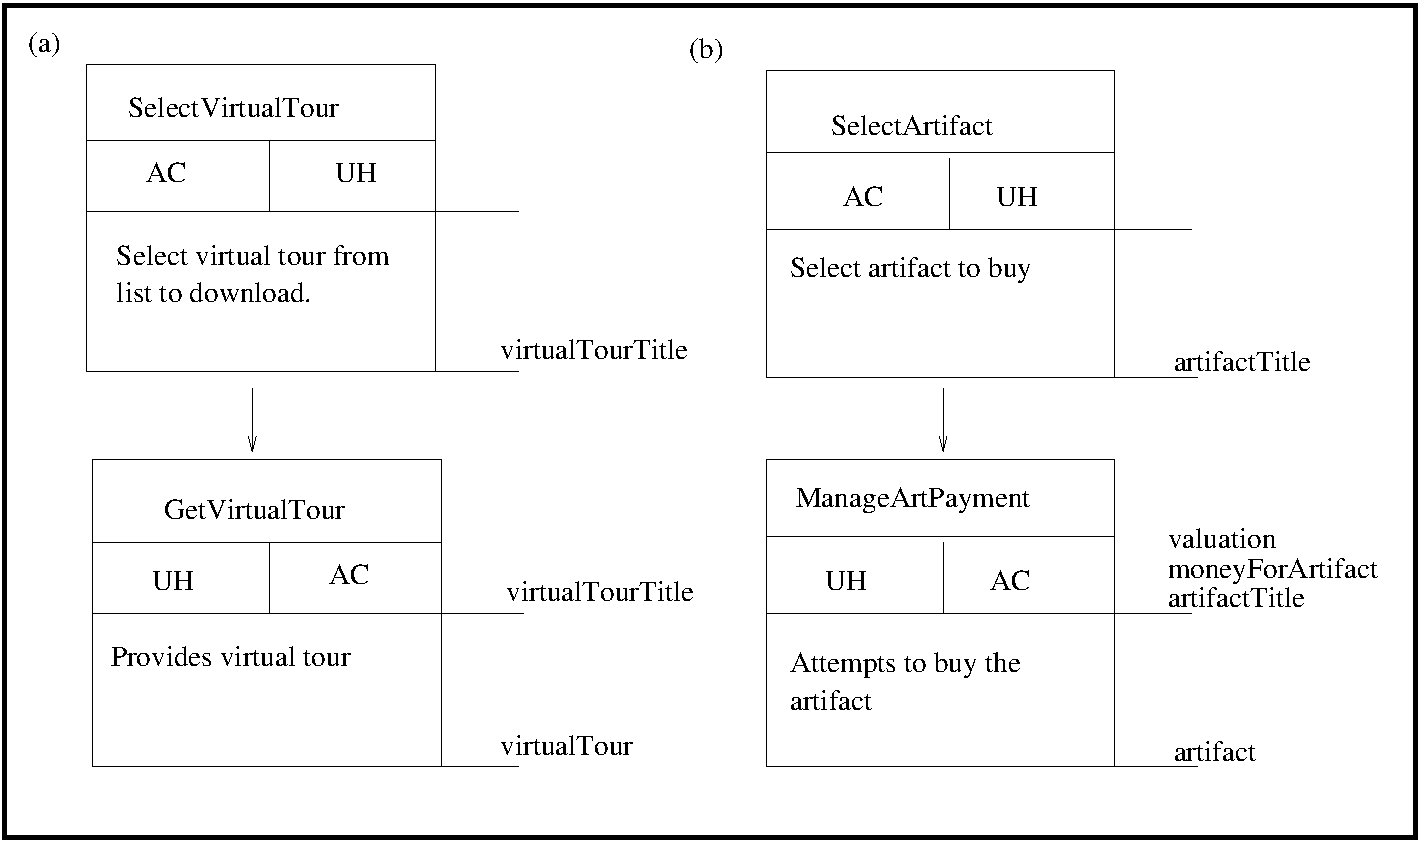
\includegraphics{ac_protocol.pdf}
    }
    \caption{Definition of protocols associated with the \textsc{ArtConsumer} role: (a) \fontfamily{\sfdefault}\selectfont DownloadVirtualTour, (b) VisitArtifact (c) BuyArt}
    \label{fig:ac_protocol}
  \end{center}
\end{figure}
\begin{figure}[H]
  \begin{center}
    \scalebox{0.70}{
      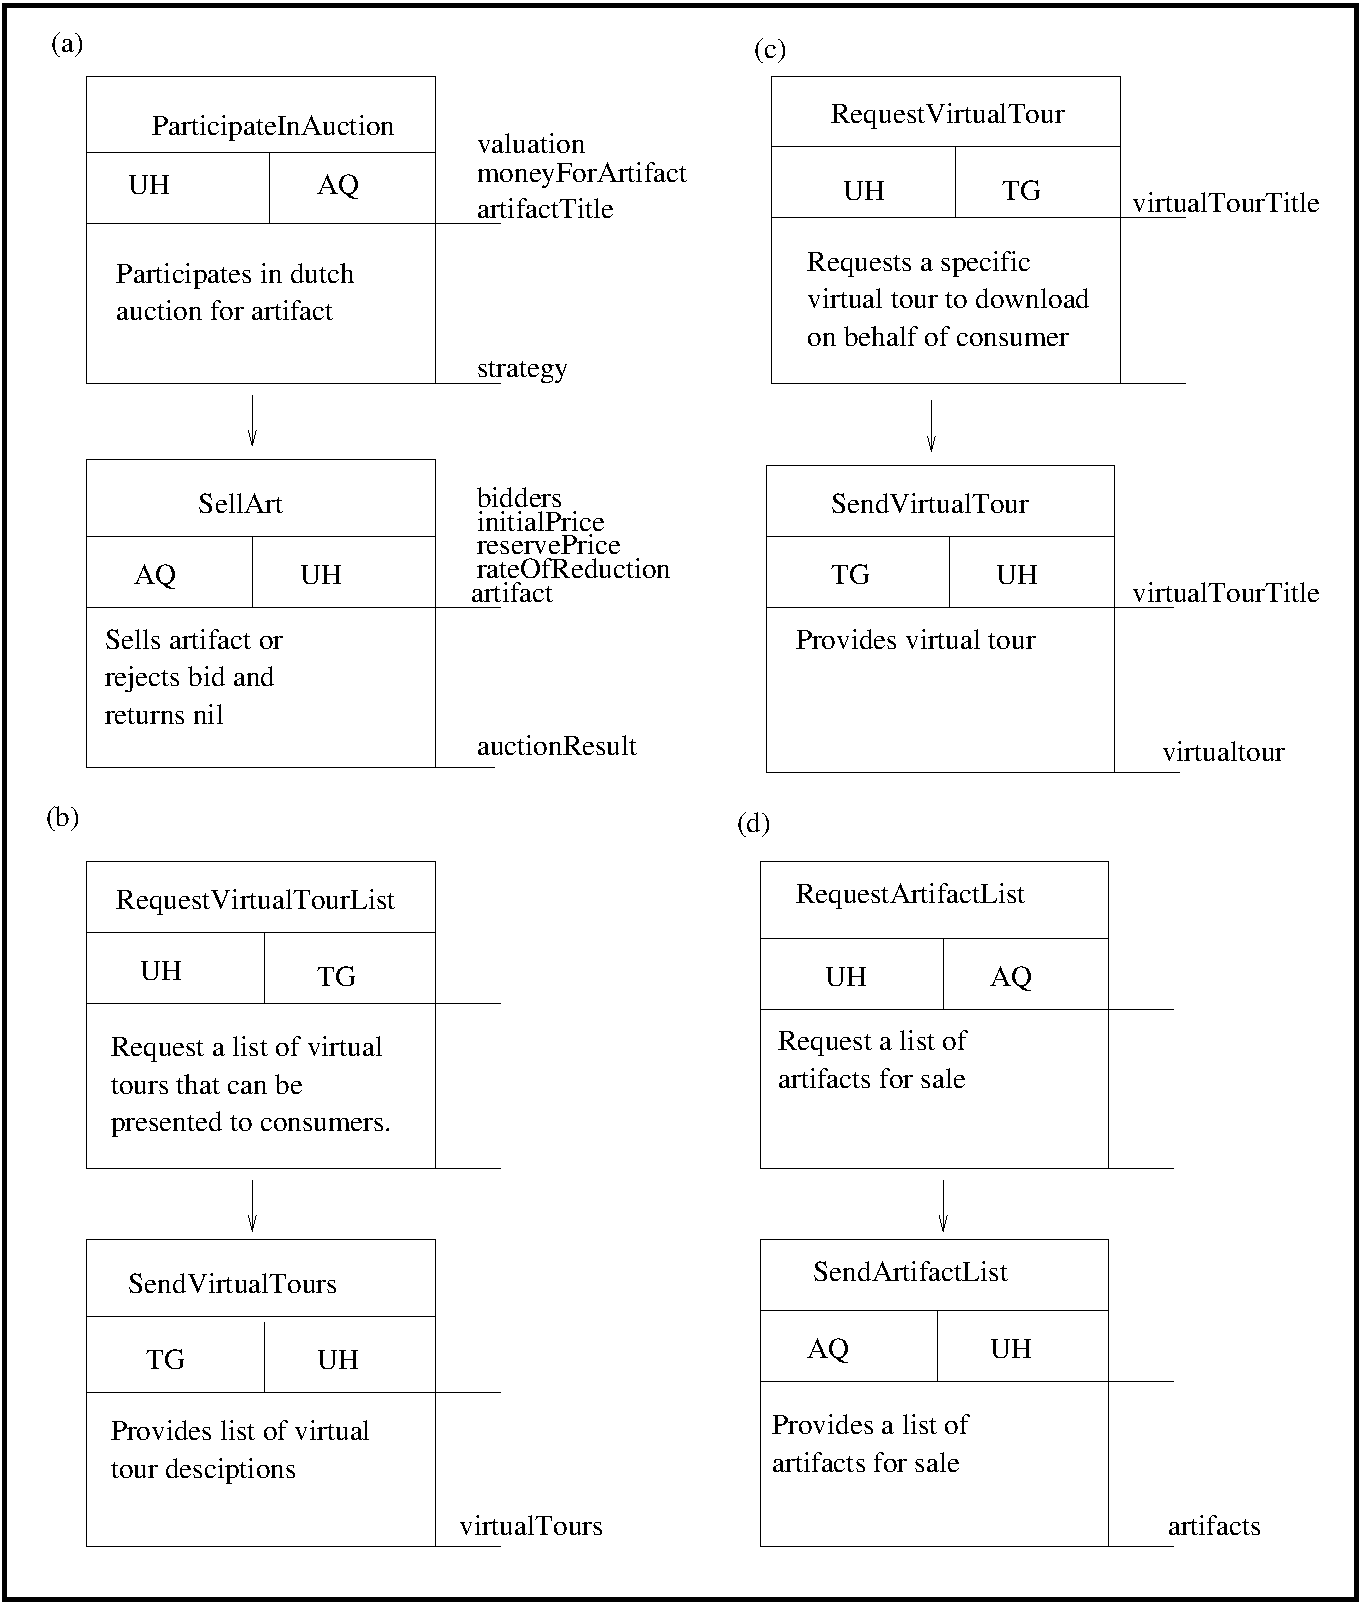
\includegraphics{uh_protocol.pdf}
    }
    \caption{Definition of protocols associated with the \textsc{UserHandler} role: (a) \fontfamily{\sfdefault}\selectfont GetArtifact, (b) GetVirtualTourList, (c) GetVirtualTour, (d) GetArtifactsList}
    \label{fig:uh_protocol}
  \end{center}
\end{figure}
\begin{figure}[H]
  \begin{center}
    \scalebox{0.70}{
      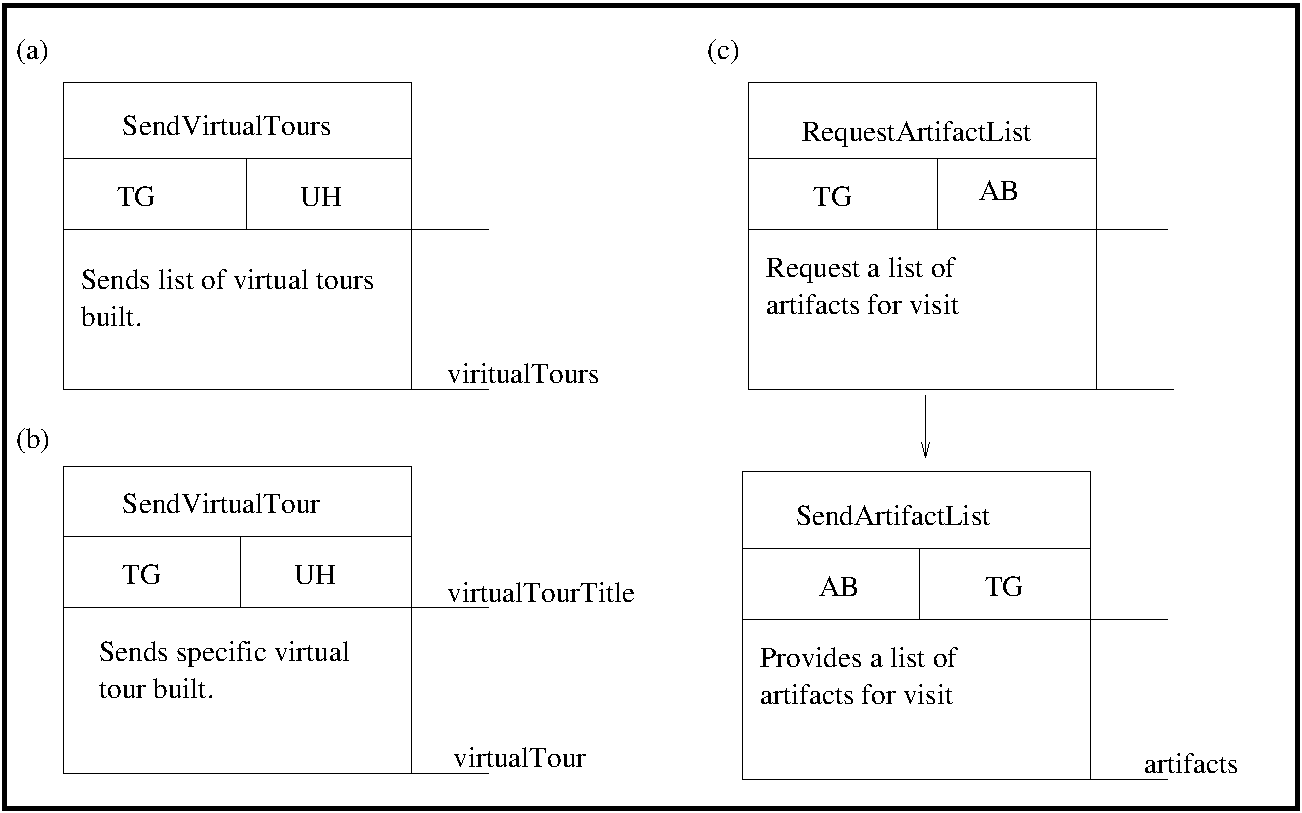
\includegraphics{tg_protocol.pdf}
    }
    \caption{Definition of protocols associated with the \textsc{TourGuide} role: (a) \fontfamily{\sfdefault}\selectfont SendVirtualTours, (b) SendVirtualTour, (c) GetArtifactList}
    \label{fig:tg_protocol}
  \end{center}
\end{figure}
\begin{figure}[H]
  \begin{center}
    \scalebox{0.70}{
      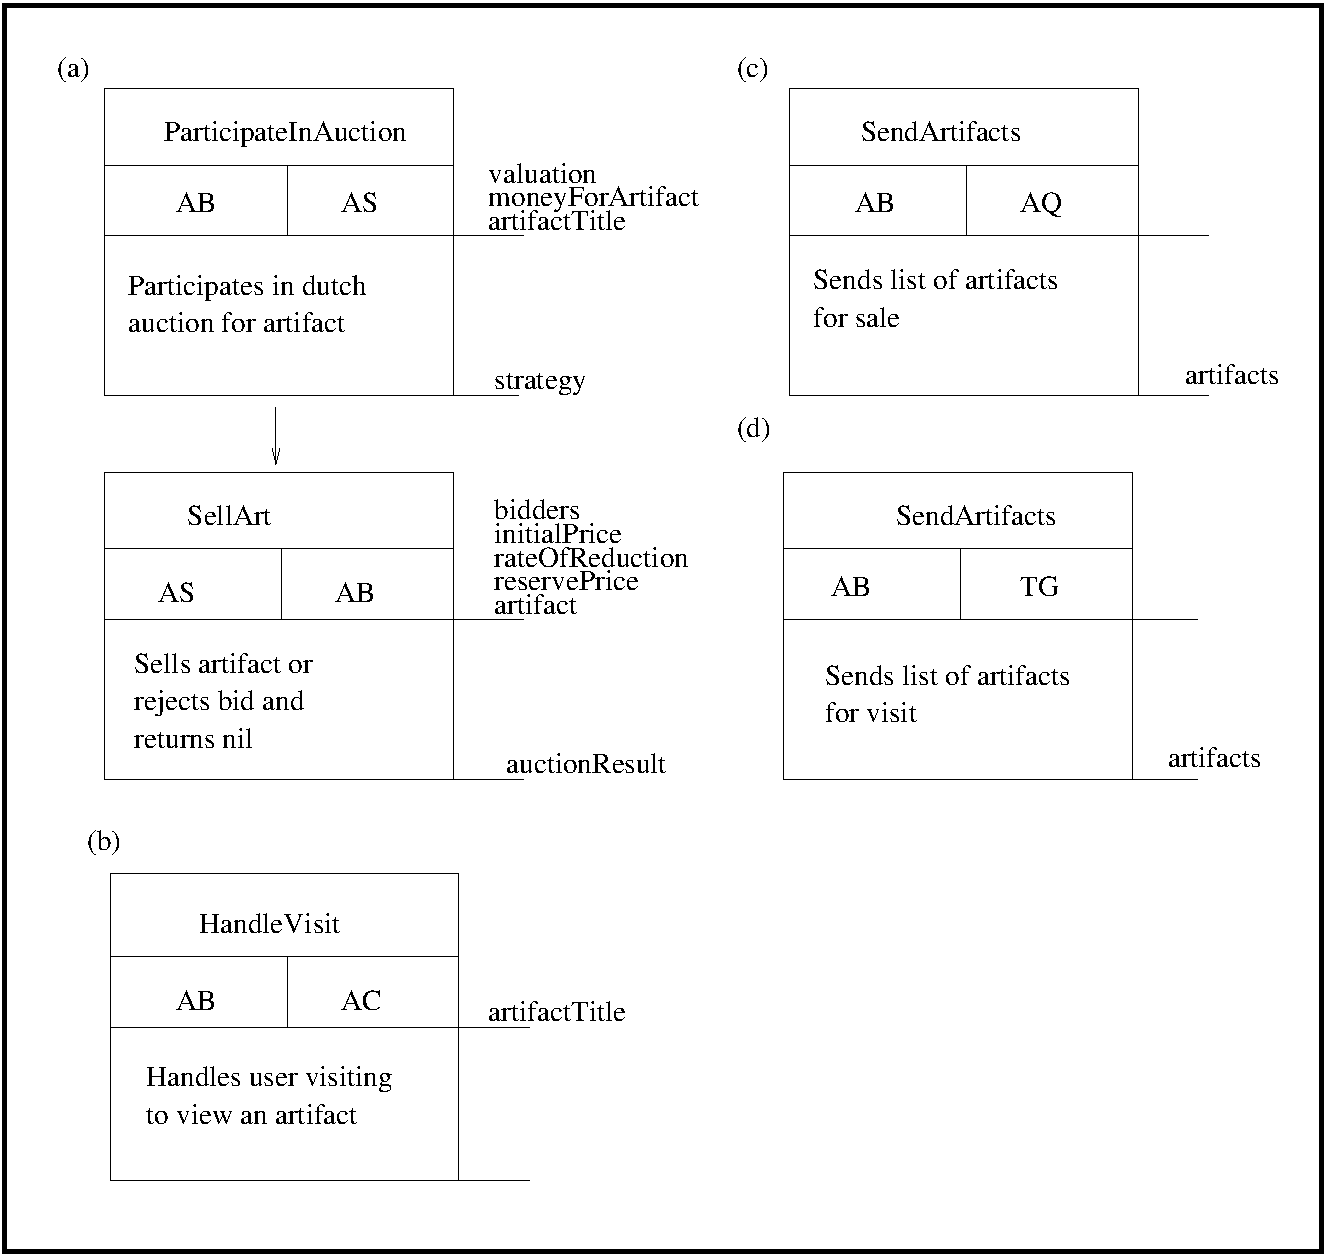
\includegraphics{ab_protocol.pdf}
    }
    \caption{Definition of protocols associated with the \textsc{ArtBuyer} role: (a) \fontfamily{\sfdefault}\selectfont BuyArt, (b) HandleVisit, (c) SendArtifacts (1), (d) SendArtifacts (2)}
    \label{fig:ab_protocol}
  \end{center}
\end{figure}

\begin{figure}[H]
  \begin{center}
    \scalebox{0.70}{
      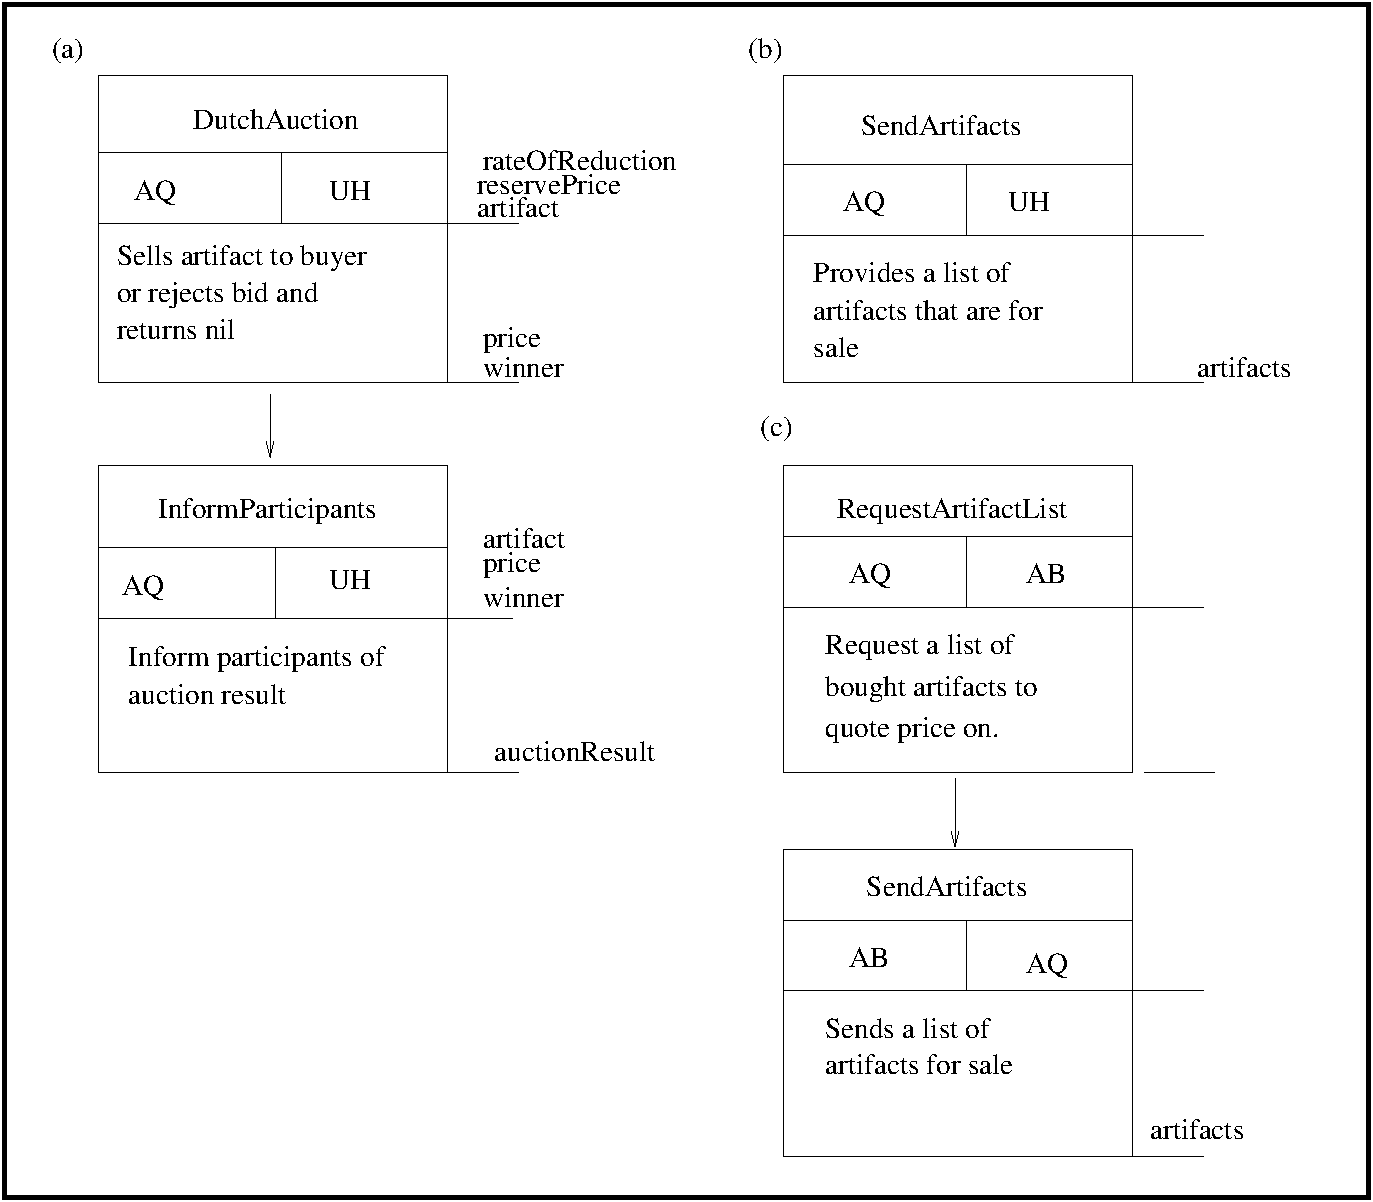
\includegraphics{aq_protocol.pdf}
    }
    \caption{Definition of protocols associated with the \textsc{ArtQuoter} role: \fontfamily{\sfdefault}\selectfont (a) SellArt, (b) SendArtifacts, (c) GetArtifacts}
    \label{fig:aq_protocol}
  \end{center}
\end{figure}
\begin{figure}[H]
  \begin{center}
    \scalebox{0.70}{
      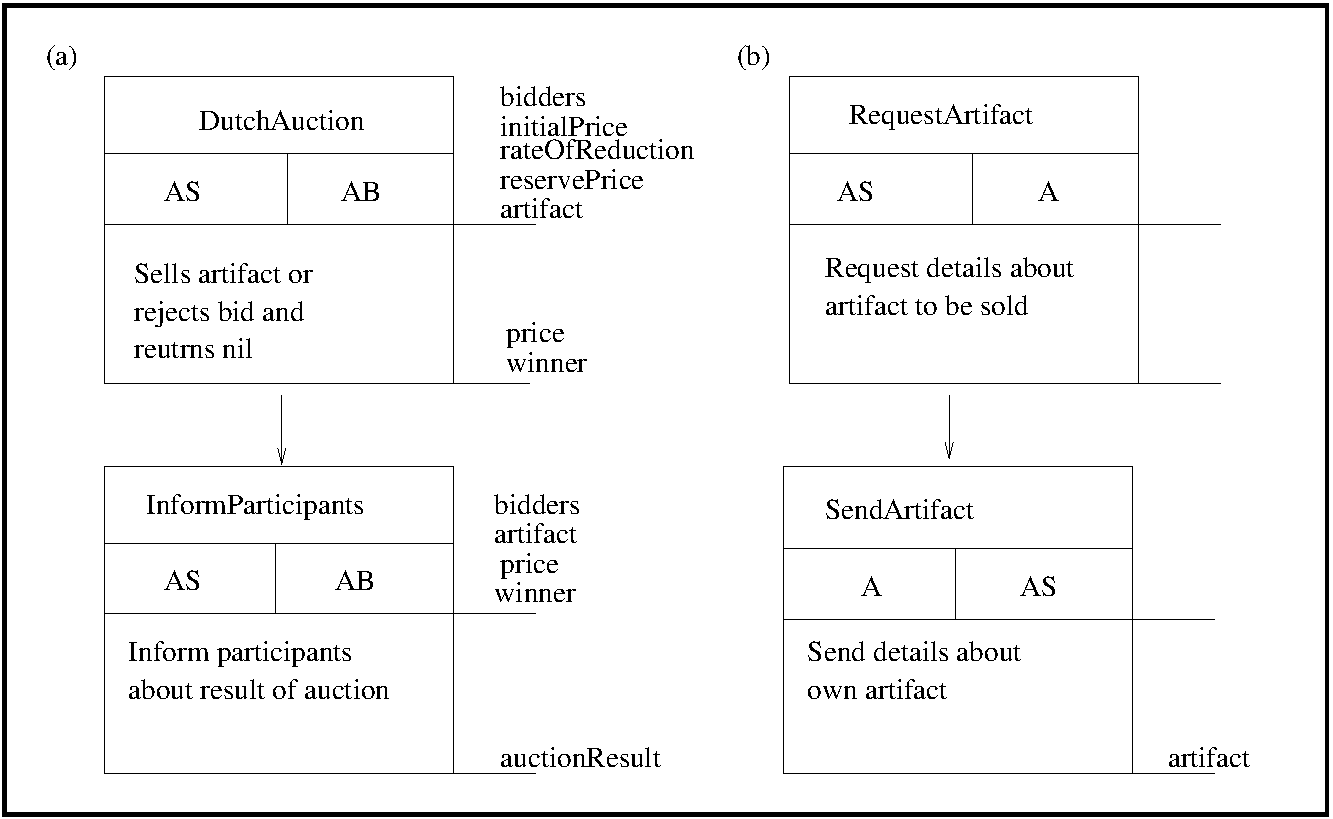
\includegraphics{as_protocol.pdf}
    }
    \caption{Definition of protocols associated with the \textsc{ArtSeller} role: \fontfamily{\sfdefault}\selectfont (a) SellArt, (b) GetArtifact}
    \label{fig:as_protocol}
  \end{center}
\end{figure}
\begin{figure}[H]
  \begin{center}
    \scalebox{0.70}{
      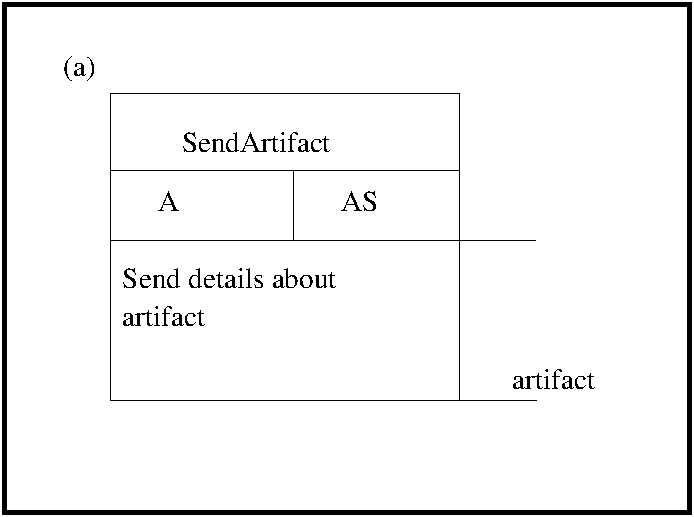
\includegraphics{a_protocol.pdf}
    }
    \caption{Definition of protocols associated with the \textsc{Artist} role: \fontfamily{\sfdefault}\selectfont (a) SendArtifact}
    \label{fig:a_protocol}
  \end{center}
\end{figure}
\subsection{Design}
\subsubsection{Agent Model}
\begin{figure}[H]
  \begin{center}
    \scalebox{0.70}{
      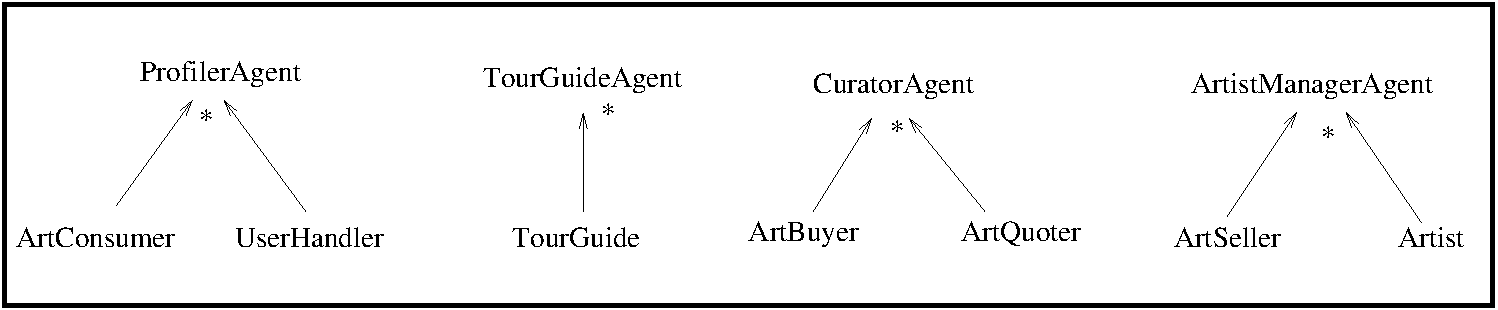
\includegraphics{agent_model.pdf}
    }
    \caption{The agent model}
    \label{fig:agent_model}
  \end{center}
\end{figure}

\subsubsection{Services Model}
\begin {table}[H]
\caption {Services model for agent \textsc{ProfilerAgent}} \label{tab:profilerAgent} 
\begin{center}
    \begin{tabular}{  p{3cm}  p{2cm}  p{2.5cm}  p{4cm}  p{4cm} }
\Xhline{4\arrayrulewidth}
    Service & Inputs & Outputs & Pre-condition & Post-condition\\ \hline
obtain virtual-tour list & & $virtualTours$ & \textbf{true} & $virtualTours \neq nil$ \\
obtain artifact list & & $artifacts$ & \textbf{true} & $artifacts \neq nil$ \\
generate list of services & $virtualTours$ $,artifacts$ & $availableServices$ & $\exists virtualTours, artifacts$ & created list of available services\\
register as bidder for auction & $auctioneer, artifact$ & & auction exists & $self \in auctioneer.bidders \land strategy \neq nil$ \\
receive CFP & currentPrice & & is participating in the auction &  \textbf{true}\\
place bid & currentPrice & & $currentPrice \leq moneyForArtifact$ & bid sent to auctioneer\\
receive bid result & $accept \lor reject$ & & have bidded & bid accepted or rejected\\
informed auction ended & $artifact \lor nil$ & & participated in auction & informed auction ended and received result\\
download virtual tour & $tourguide, virtualtour$ & & $\exists tourguide, virtualtour$ & downloaded virtual tour\\
visitArtifact & $curator, artifactTitle$ & & $artifactTitle \in curator.gallery.titles$ & $artifactTitle \in visitedArtifacts$\\
\Xhline{4\arrayrulewidth}
    \end{tabular}
\end{center}
\end{table}

\begin {table}[H]
\caption {Services model for agent \textsc{TourGuideAgent}} \label{tab:tourguideAgent} 
\begin{center}
    \begin{tabular}{  p{3cm}  p{2.5cm}  p{2.5cm}  p{4cm}  p{4cm} }
\Xhline{4\arrayrulewidth}
    Service & Inputs & Outputs & Pre-condition & Post-condition\\ \hline
obtain artifact list & & $artifacts$ & \textbf{true} & $artifacts \neq nil$ \\
manage virtual-tour request & $virtualTourTitle$& $virtualTour \lor nil$ & \textbf{true} & \textbf{true} \\
manage list of virtual-tours-request & & $virtualTours$ & \textbf{true} & \textbf{true} \\
build virtual tour & $artifacts$ & $virtualTour$ & $artifacts.size > 0$ & $virtualTour \neq nil$ \\
\Xhline{4\arrayrulewidth}
    \end{tabular}
\end{center}
\end{table}

\begin {table}[H]
\caption {Services model for agent \textsc{ArtistManagerAgent}} \label{tab:artistmanagerAgent} 
\begin{center}
    \begin{tabular}{  p{3cm}  p{2.5cm}  p{2.5cm}  p{4cm}  p{4cm} }
\Xhline{4\arrayrulewidth}
    Service & Inputs & Outputs & Pre-condition & Post-condition\\ \hline
get registered bidders & & $bidders$ & \textbf{true} & \textbf{true}\\
send inform-start-of-auction &$bidders$ & $informMessage$ & bidders are registered & bidders informed about start of auction \\
send CFP &$bidders$ & $CFP$ & bidders are registered and auction ongoing & bidders informed about current price and encouraged to bid \\
receive bid &$bid$ & $bids$ & bidder registered  & $bid \in bids$ \\
manage bids &$bids$ & $bidResponses$ & $bids > 0$ & one bid was accepted and the bidder received the good, the rest was rejected and the bidders were informed \\
modify price &$reservePrice,$ $rateOfReduction,$ $currentPrice$ & $newPrice$& no bids was received & $reservePrice \leq newPrice \leq currentPrice$ \\
send inform-auction-closed &$bidders$, $auctionResult$ & $informMessage$ & bidders are registered & bidders informed about close of auction \\
\Xhline{4\arrayrulewidth}
    \end{tabular}
\end{center}
\end{table}

\begin {table}[H]
\caption {Services model for agent \textsc{CuratorAgent}} \label{tab:curatorAgent} 
\begin{center}
    \begin{tabular}{  p{3cm}  p{2.5cm}  p{2.5cm}  p{4cm}  p{4cm} }
\Xhline{4\arrayrulewidth}
    Service & Inputs & Outputs & Pre-condition & Post-condition\\ \hline
get registered bidders & & $bidders$ & \textbf{true} & \textbf{true}\\
register as bidder for auction & $auctioneer, artifact$ & & auction exists & $self \in auctioneer.bidders \land strategy \neq nil$ \\
receive CFP & currentPrice & & is participating in the auction &  \textbf{true}\\
place bid & currentPrice & & $currentPrice \leq moneyForArtifact$ & bid sent to auctioneer\\
receive bid result & $accept \lor reject$ & & have bidded & bid accepted or rejected\\
informed auction ended & $artifact \lor nil$ & & participated in auction & curator were informed auction ended and received result\\
manage artifact-list request & & $artifacts$ & \textbf{true} & \textbf{true}\\
manage visit-artifact request &$artifactTitle$ & $artifact$ & \textbf{true} & provided artifact for visit only\\
quote art &$artifact$ & $quote$ & \textbf{true} & \textbf{true} \\
send inform-start-of-auction &$bidders$ & $informMessage$ & bidders are registered & bidders informed about start of auction \\
send CFP &$bidders$ & $CFP$ & bidders are registered and auction ongoing & bidders informed about current price and encouraged to bid \\
receive bid &$bid$ & $bids$ & bidder registered  & $bid \in bids$ \\
manage bids &$bids$ & $bidResponses$ & $bids > 0$ & one bid was accepted and the bidder received the good, the rest was rejected and the bidders were informed \\
modify price &$reservePrice,$ $rateOfReduction,$ $currentPrice$ & $newPrice$& no bids was received & $reservePrice \leq newPrice \leq currentPrice$ \\
send inform-auction-closed &$bidders$, $auctionResult$ & $informMessage$ & bidders are registered & bidders informed about close of auction \\
\Xhline{4\arrayrulewidth}
    \end{tabular}
\end{center}
\end{table}

\subsubsection{Acquaintance Model}
\begin{figure}[H]
  \begin{center}
    \scalebox{0.70}{
      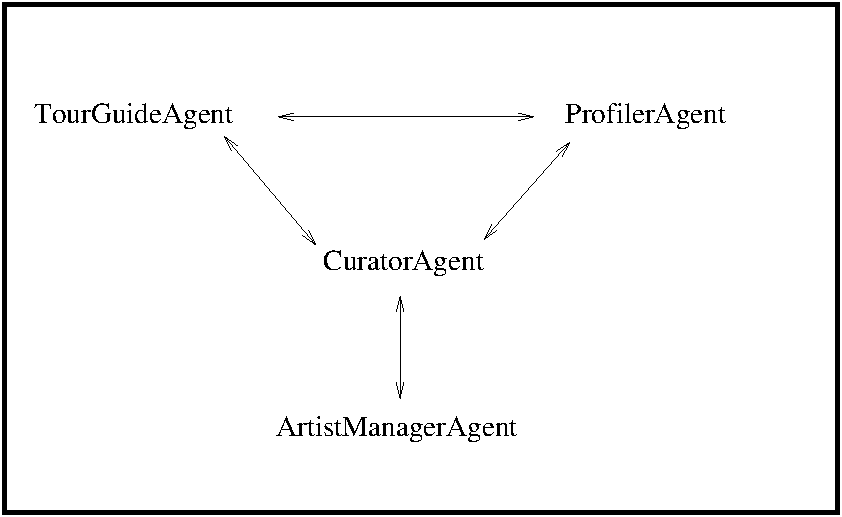
\includegraphics{acquaintance_model.pdf}
    }
    \caption{Acquaintance model}
    \label{fig:acquaintance_model}
  \end{center}
\end{figure}

\subsubsection{Mobility Model}
\begin{assumption}{2}{A}\label{2A}
I've assumed the mobile architecture that I used for homework 3, i.e that only artistmanager agents and curator agents are mobile and can clone themself. Further more the cardinality of agents and places also follow from this assumption.
\end{assumption}
\begin {table}[H]
\caption {Place Types} \label{tab:placeTypes} 
\begin{center}
    \begin{tabular}{  p{4cm}  p{4cm}  p{4cm} }
\Xhline{4\arrayrulewidth}
    Place Types & Description & Instances \\ \hline
Heritage Malta Container & Container where art-curators can reside and perform their services and where artistmanager agents can reside temporarily to perform auctions & 1 \\
Museo Galileo Container & Container where art-curators can reside and perform their services and where artistmanager agents can reside temporarily to perform auctions & 1 \\
ArtistManager Container & Container where artistmanager agents reside and where they come back to after performing auctions & * \\
ProfilerAgent Container & Container where profiler agents reside  & * \\ 
TourGuideAgent Container & Container where tourguide agents reside  & * \\ 
\Xhline{4\arrayrulewidth}
    \end{tabular}
\end{center}
\end{table}

\begin {table}[H]
\caption {Agents and Places Specification} \label{tab:placeTypes} 
\begin{center}
    \begin{tabular}{  p{4cm}  p{4cm}  p{4cm} p{4cm}}
\Xhline{4\arrayrulewidth}
    Agent Type & Mobile & Place Type & Constraints \\
 \hline
ProfilerAgent & No & ProfilerAgent Container & \\
TourGuideAgent & No & TourGuideAgent Container & \\
CuratorAgent & Yes & Museo Galileo Container, Heritage Malta Container & \\
ArtistManagerAgent & Yes & ArtistManagerAgentContainer, Museo Galileo Container, Heritage Malta Container &  \\

\Xhline{4\arrayrulewidth}
    \end{tabular}
\end{center}
\end{table}

\begin{figure}[H]
  \begin{center}
    \scalebox{0.70}{
      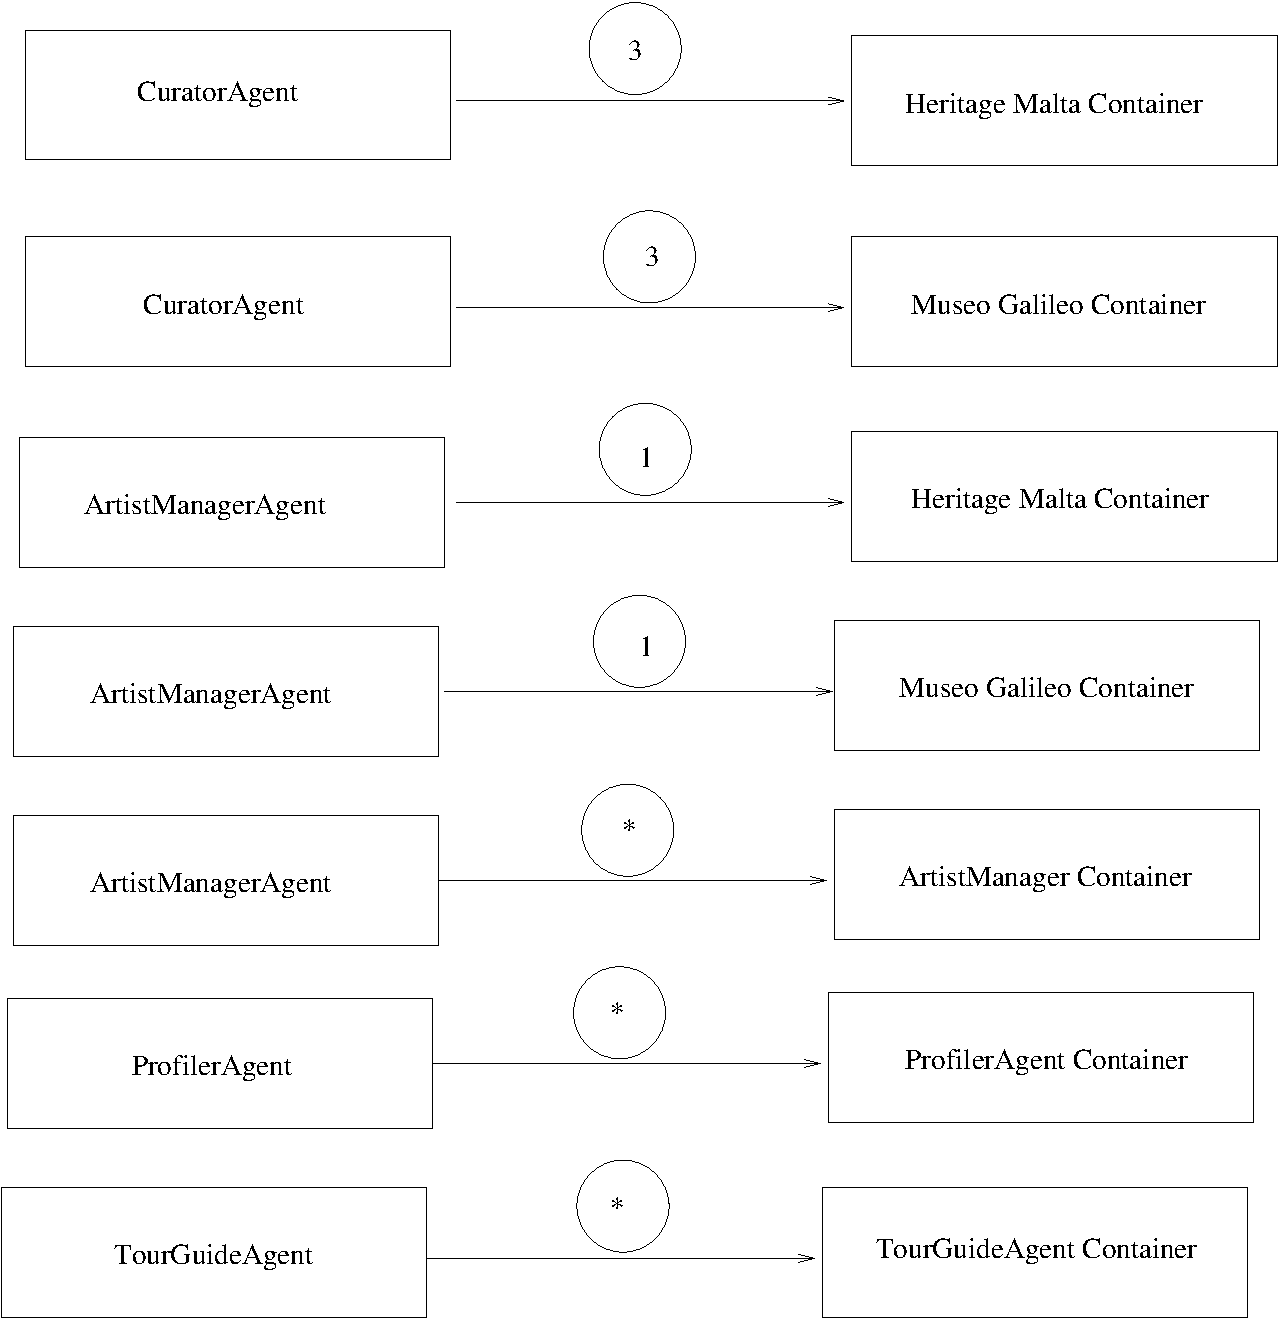
\includegraphics{cardinality.pdf}
    }
    \caption{Cardinality of Agents and Places}
    \label{fig:cardinality}
  \end{center}
\end{figure}

\begin{figure}[H]
  \begin{center}
\noindent\fbox{%
    \parbox{\textwidth}{%
\setlength\parindent{14pt} Agent Type: \hspace{1em} \textsc{CuratorAgent}\\
\setlength\parindent{14pt} \noindent\rule{15cm}{0.4pt}

\par \setlength\parindent{14pt} Description: \hspace{30pt}Can be cloned in current container to participate in auctions.
\par \setlength\parindent{14pt} Origin: \hspace{49pt} Heritage Malta Container or Museo Galileo Container.
\par \setlength\parindent{14pt} Final Destination: \hspace{6pt}Same as its origin container.
\par \setlength\parindent{14pt} List of atomic movements:
\\
\par \setlength\parindent{44pt}\fbox{%
    \parbox{300pt}{%
\hspace{10pt} 1 \hspace{15pt} \vrule  \hspace{10pt} Cloned in Heritage Malta Container
    }%
}
\par \setlength\parindent{44pt}\fbox{%
    \parbox{300pt}{%
\hspace{10pt} 2 \hspace{15pt} \vrule  \hspace{10pt} Cloned in Museo Galileo Container
    }%
}
\\
\setlength\parindent{14pt} \noindent\rule{15cm}{0.4pt}

\par \setlength\parindent{14pt} Paths: 
\par \setlength\parindent{104pt} Cloned in the same container, no paths.
    }%
}
\caption{Travel schema for agent\textsc{CuratorAgent}}
\label{fig:travel_schema_curator}
\end{center}
\end{figure}

\begin{figure}[H]
  \begin{center}
\noindent\fbox{%
    \parbox{\textwidth}{%
\setlength\parindent{14pt} Agent Type: \hspace{1em} \textsc{ArtistManagerAgent}\\
\setlength\parindent{14pt} \noindent\rule{15cm}{0.4pt}

\par \setlength\parindent{14pt} Description: \hspace{30pt}Can move between Museo Galileo Container, Heritage Malta Container
\par \setlength\parindent{104pt} and ArtistManager Container.
\par \setlength\parindent{14pt} Origin: \hspace{49pt} ArtistManager Container
\par \setlength\parindent{14pt} Final Destination: \hspace{6pt}ArtistManager Container
\par \setlength\parindent{14pt} List of atomic movements:
\\
\par \setlength\parindent{44pt}\fbox{%
    \parbox{320pt}{%
\hspace{5pt} 1 \hspace{5pt} \vrule  \hspace{10pt} Move from ArtistManager to Heritage Malta Container.
    }%
}
\par \setlength\parindent{44pt}\fbox{%
    \parbox{320pt}{%
\hspace{5pt} 2 \hspace{5pt} \vrule  \hspace{10pt} Move from Heritage Malta to ArtistManager Container.
    }%
}
\par \setlength\parindent{44pt}\fbox{%
    \parbox{320pt}{%
\hspace{5pt} 3 \hspace{5pt} \vrule  \hspace{10pt} Move from ArtistManager to Museo Galieo Container.
    }%
}

\par \setlength\parindent{44pt}\fbox{%
    \parbox{320pt}{%
\hspace{5pt} 4 \hspace{5pt} \vrule  \hspace{10pt} Move from Museo Galieo to ArtistManager Container.
    }%
}

\par \setlength\parindent{44pt}\fbox{%
    \parbox{320pt}{%
\hspace{5pt} 5 \hspace{5pt} \vrule  \hspace{10pt} Move from Museo Galieo to Heritage Malta Container.
    }%
}

\par \setlength\parindent{44pt}\fbox{%
    \parbox{320pt}{%
\hspace{5pt} 6 \hspace{5pt} \vrule  \hspace{10pt} Move from Heritage Malta to Museo Galieo Container.
    }%
}
\\
\setlength\parindent{14pt} \noindent\rule{15cm}{0.4pt}

\par \setlength\parindent{14pt} Paths: 
\\
\par \setlength\parindent{44pt}\fbox{%
    \parbox{300pt}{%
\hspace{10pt} 1 \hspace{15pt} \vrule  \hspace{10pt} 1.2
    }%
}
\par \setlength\parindent{44pt}\fbox{%
    \parbox{300pt}{%
\hspace{10pt} 1 \hspace{15pt} \vrule  \hspace{10pt} 3.4
    }%
}

\par \setlength\parindent{44pt}\fbox{%
    \parbox{300pt}{%
\hspace{10pt} 1 \hspace{15pt} \vrule  \hspace{10pt} 1.6
    }%
}

\par \setlength\parindent{44pt}\fbox{%
    \parbox{300pt}{%
\hspace{10pt} 1 \hspace{15pt} \vrule  \hspace{10pt} 3.5
    }%
}

\par \setlength\parindent{44pt}\fbox{%
    \parbox{300pt}{%
\hspace{10pt} 1 \hspace{15pt} \vrule  \hspace{10pt} 3.5.2
    }%
}
\par \setlength\parindent{44pt}\fbox{%
    \parbox{300pt}{%
\hspace{10pt} 1 \hspace{15pt} \vrule  \hspace{10pt} 1.6.4
    }%
}


    }%
}
\caption{Travel schema for agent\textsc{ArtistManagerAgent}}
\label{fig:travel_schema_artistmanager}
\end{center}
\end{figure}

\begin{figure}[H]
  \begin{center}
\noindent\fbox{%
    \parbox{\textwidth}{%
\setlength\parindent{14pt} Agent Type: \hspace{1em} \textsc{ProfilerAgent}\\
\setlength\parindent{14pt} \noindent\rule{15cm}{0.4pt}

\par \setlength\parindent{14pt} Description: \hspace{30pt} Static agent, not mobile.
\par \setlength\parindent{14pt} Origin: \hspace{53pt} ProfilerAgentContainer
\par \setlength\parindent{14pt} Final Destination: \hspace{6pt} ProfilerAgentContainer
\par \setlength\parindent{14pt} List of atomic movements:
\par \setlength\parindent{44pt}The agent is static and don't have any atomic movements.
\\
\setlength\parindent{14pt} \noindent\rule{15cm}{0.4pt}

\par \setlength\parindent{14pt} Paths: 
\par \setlength\parindent{44pt} No paths
    }%
}
\caption{Travel schema for agent\textsc{ProfilerAgent}}
\label{fig:travel_schema_profiler}
\end{center}
\end{figure}

\begin{figure}[H]
  \begin{center}
\noindent\fbox{%
    \parbox{\textwidth}{%
\setlength\parindent{14pt} Agent Type: \hspace{1em} \textsc{TourGuideAgent}\\
\setlength\parindent{14pt} \noindent\rule{15cm}{0.4pt}

\par \setlength\parindent{14pt} Description: \hspace{30pt} Static agent, not mobile.
\par \setlength\parindent{14pt} Origin: \hspace{53pt} TourGuideAgentContainer
\par \setlength\parindent{14pt} Final Destination: \hspace{6pt} TourGuideAgentContainer
\par \setlength\parindent{14pt} List of atomic movements:
\par \setlength\parindent{44pt}The agent is static and don't have any atomic movements.
\\
\setlength\parindent{14pt} \noindent\rule{15cm}{0.4pt}

\par \setlength\parindent{14pt} Paths: 
\par \setlength\parindent{44pt} No paths
    }%
}
\caption{Travel schema for agent\textsc{TourGuideAgent}}
\label{fig:travel_schema_tourguide}
\end{center}
\end{figure}
\section{Task 2 - Modeling with AgentUML}
An alternative to the GAIA modeling approach is stick to UML, which is the dominant way of modeling in general software engineering and in particular object-oriented areas. However in the context of agent-oriented programing the UML standard have some obvious problems which are to be expected since UML was not designed for agent-oriented programming but rather object-oriented. Agent UML is an extension to UML with the purpose of making UML more usable for agent-based systems. In this section the result of modeling the SmartMuseum framework with the AgentUML method, and specifically with the approach used in \citep{agent_uml1} is presented.
\subsection{The Overall Protocol}
\subsubsection{ArtistManager Auction package}
High-level overview of the protocol where ArtistManagerAgents auctions art-artifacts to CuratorAgents using dutch auctions.
\begin{figure}[H]
  \begin{center}
    \scalebox{0.70}{
      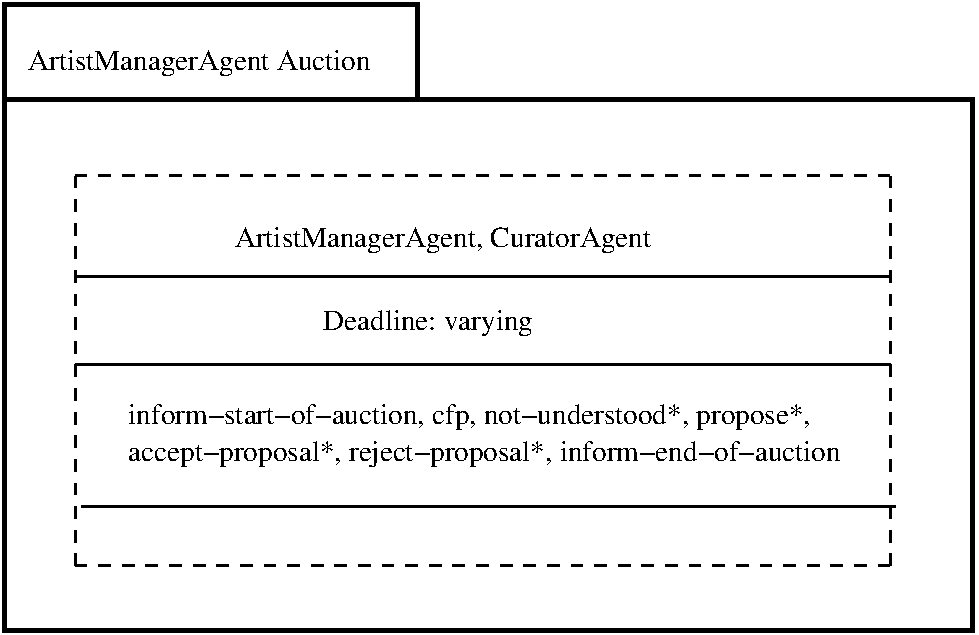
\includegraphics{artist_auction_template.pdf}
    }
    \caption{ArtistManager Auction package}
    \label{fig:artist_auction_template}
  \end{center}
\end{figure}
\subsubsection{Curator Auction package}
High-level overview of the protocol where CuratorAgents auctions art-artifacts to ProfilerAgents using dutch auctions.
\begin{figure}[H]
  \begin{center}
    \scalebox{0.70}{
      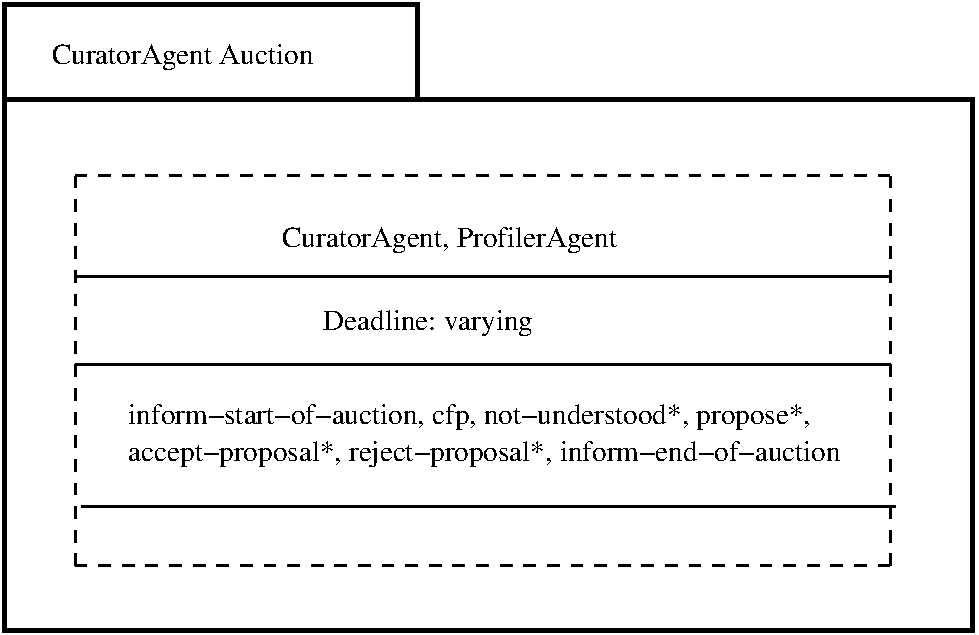
\includegraphics{curator_auction_template.pdf}
    }
    \caption{Curator Auction package}
    \label{fig:curator_auction_template}
  \end{center}
\end{figure}

\subsubsection{BuildVirtualTour package}
High-level overview of the protocol where TourGuideAgents sonds the terrain of artifacts at different curators and then build virtual tours of different type.
\begin{figure}[H]
  \begin{center}
    \scalebox{0.70}{
      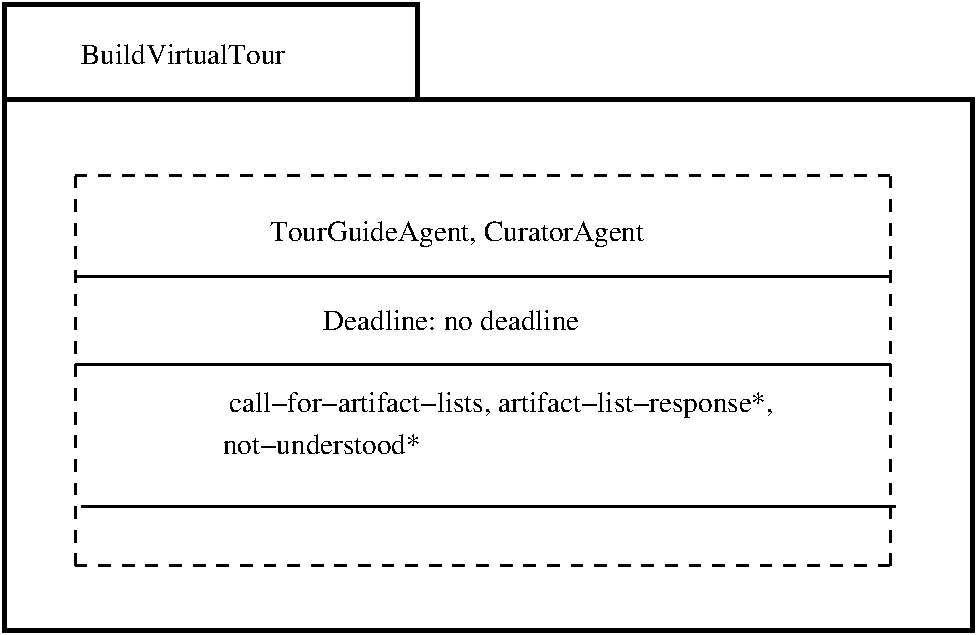
\includegraphics{build_virtual_tour_temp.pdf}
    }
    \caption{BuildVirtualTour package}
    \label{fig:build_virtual_tour_temp}
  \end{center}
\end{figure}

\subsubsection{FindVirtualTour package}
High-level overview of the protocol where ProfilerAgents searches for virtual tours and rejects or selects the virtual tours.
\begin{figure}[H]
  \begin{center}
    \scalebox{0.70}{
      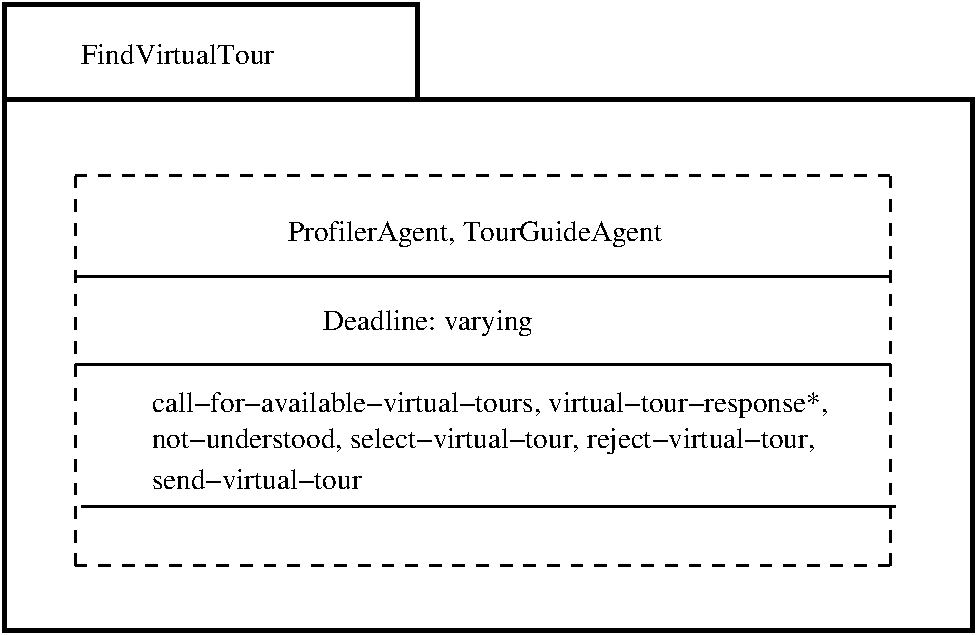
\includegraphics{find_virtual_tour.pdf}
    }
    \caption{FindVirtualTour package}
    \label{fig:find_virtual_tour}
  \end{center}
\end{figure}
\subsubsection{VisitArtifact package}
High-level overview of the protocol where ProfilerAgents visits artifacts from a virtual tour.
\begin{figure}[H]
  \begin{center}
    \scalebox{0.7}{
      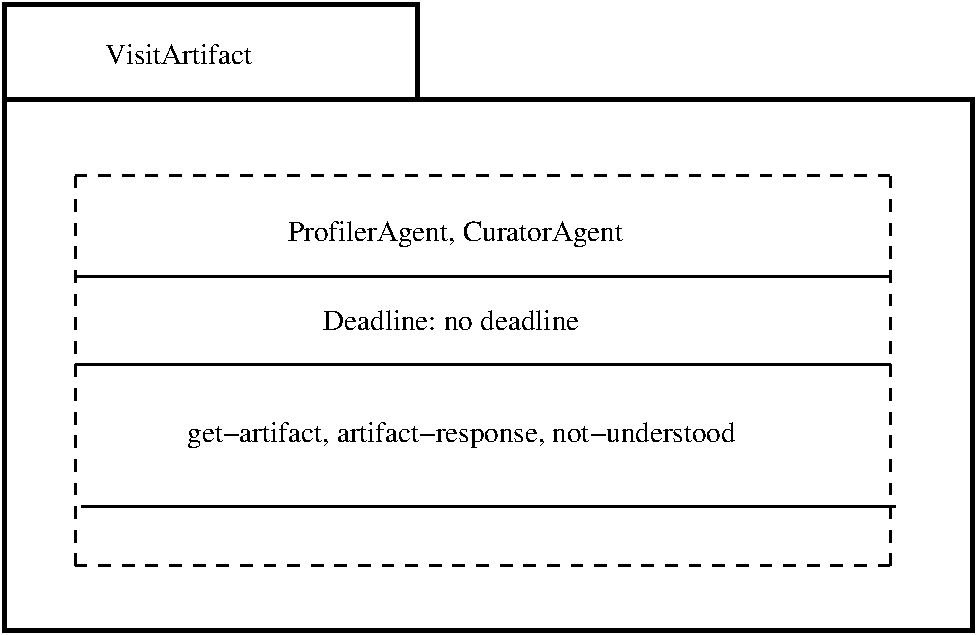
\includegraphics{visit_artifact.pdf}
    }
    \caption{VisitArtifact package}
    \label{fig:visit_artifact}
  \end{center}
\end{figure}
\subsection{Interactions Among Agents}
\subsubsection{ArtistManagerAgent Auction}
Sequence diagram over the ArtistManagerAgent Auction protocol. When invoked the ArtistManagerAgent sends an $inform-start-of-auction$ message to $n$ number of CuratorAgents, then it sends a call for proposal  with the current price,  $cfp-1$ to $n$ CuratorAgents. CuratorAgents can then either not respond at all or respond with either $not-understood$ or $propose$. The diamond and $X$ indicates that one of the two choices, exlusive, need to be taken. The ArtistManagerAgent will then correspondingly take different action based on which response it receives. If it receives a $not-understood$ response it does nothing, if it receives a $propose$ response (bid) it will either reject or accept it. Finally if the ArtistManagerAgent did'nt receive any bids for a certain amount of time it can either send out another $cfp$ or close the auction by sending a $inform-end-of-auction$ message in case the reservedPrice was reached.
\begin{figure}[H]
  \begin{center}
    \scalebox{0.70}{
      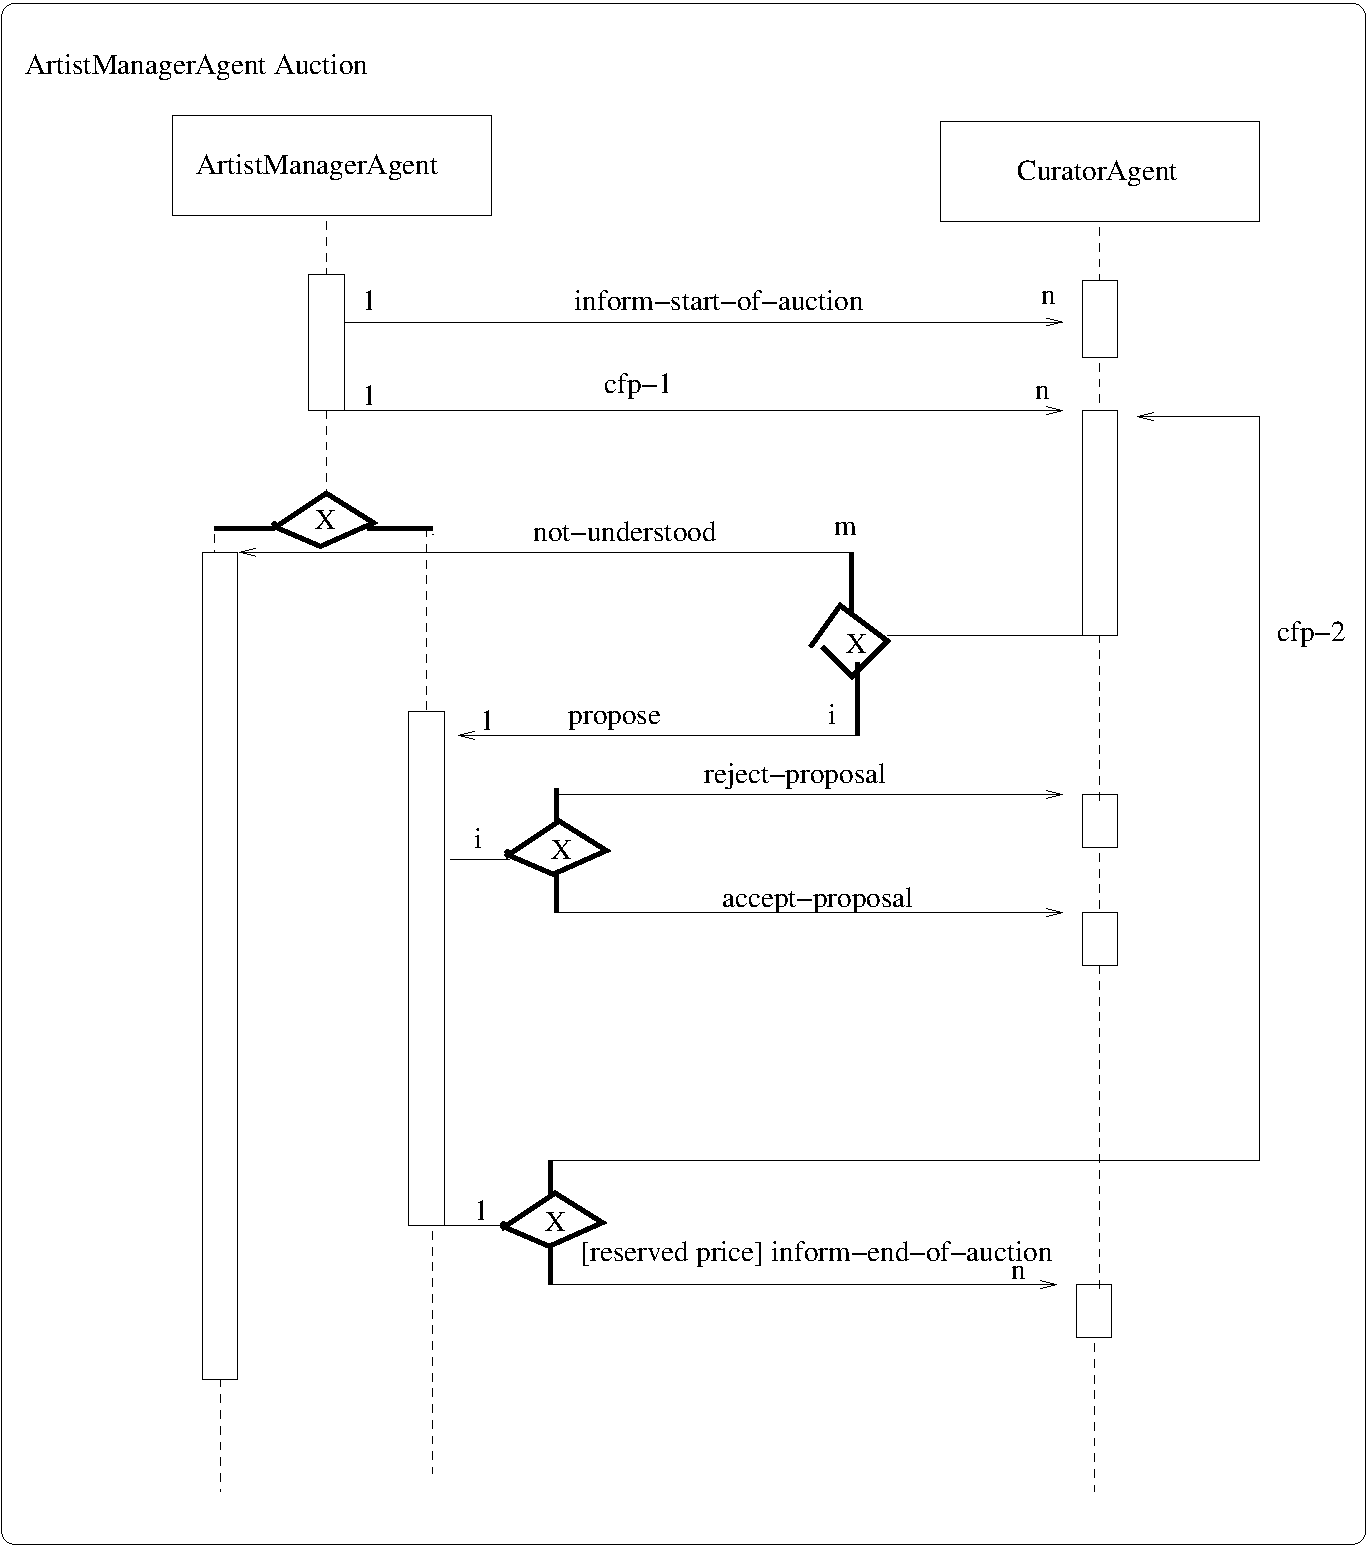
\includegraphics{artist_auction_sequence.pdf}
    }
    \caption{Sequence diagram over the interaction for ArtistManagerAgent Auction}
    \label{fig:artist_auction_sequence}
  \end{center}
\end{figure}
\subsubsection{CuratorAgent Auction}
Sequence diagram over the CuratorAgent Auction protocol, this protocol follows the same dutch auction protocol as ArtistManagerAgentProtocol.
\begin{figure}[H]
  \begin{center}
    \scalebox{0.69}{
      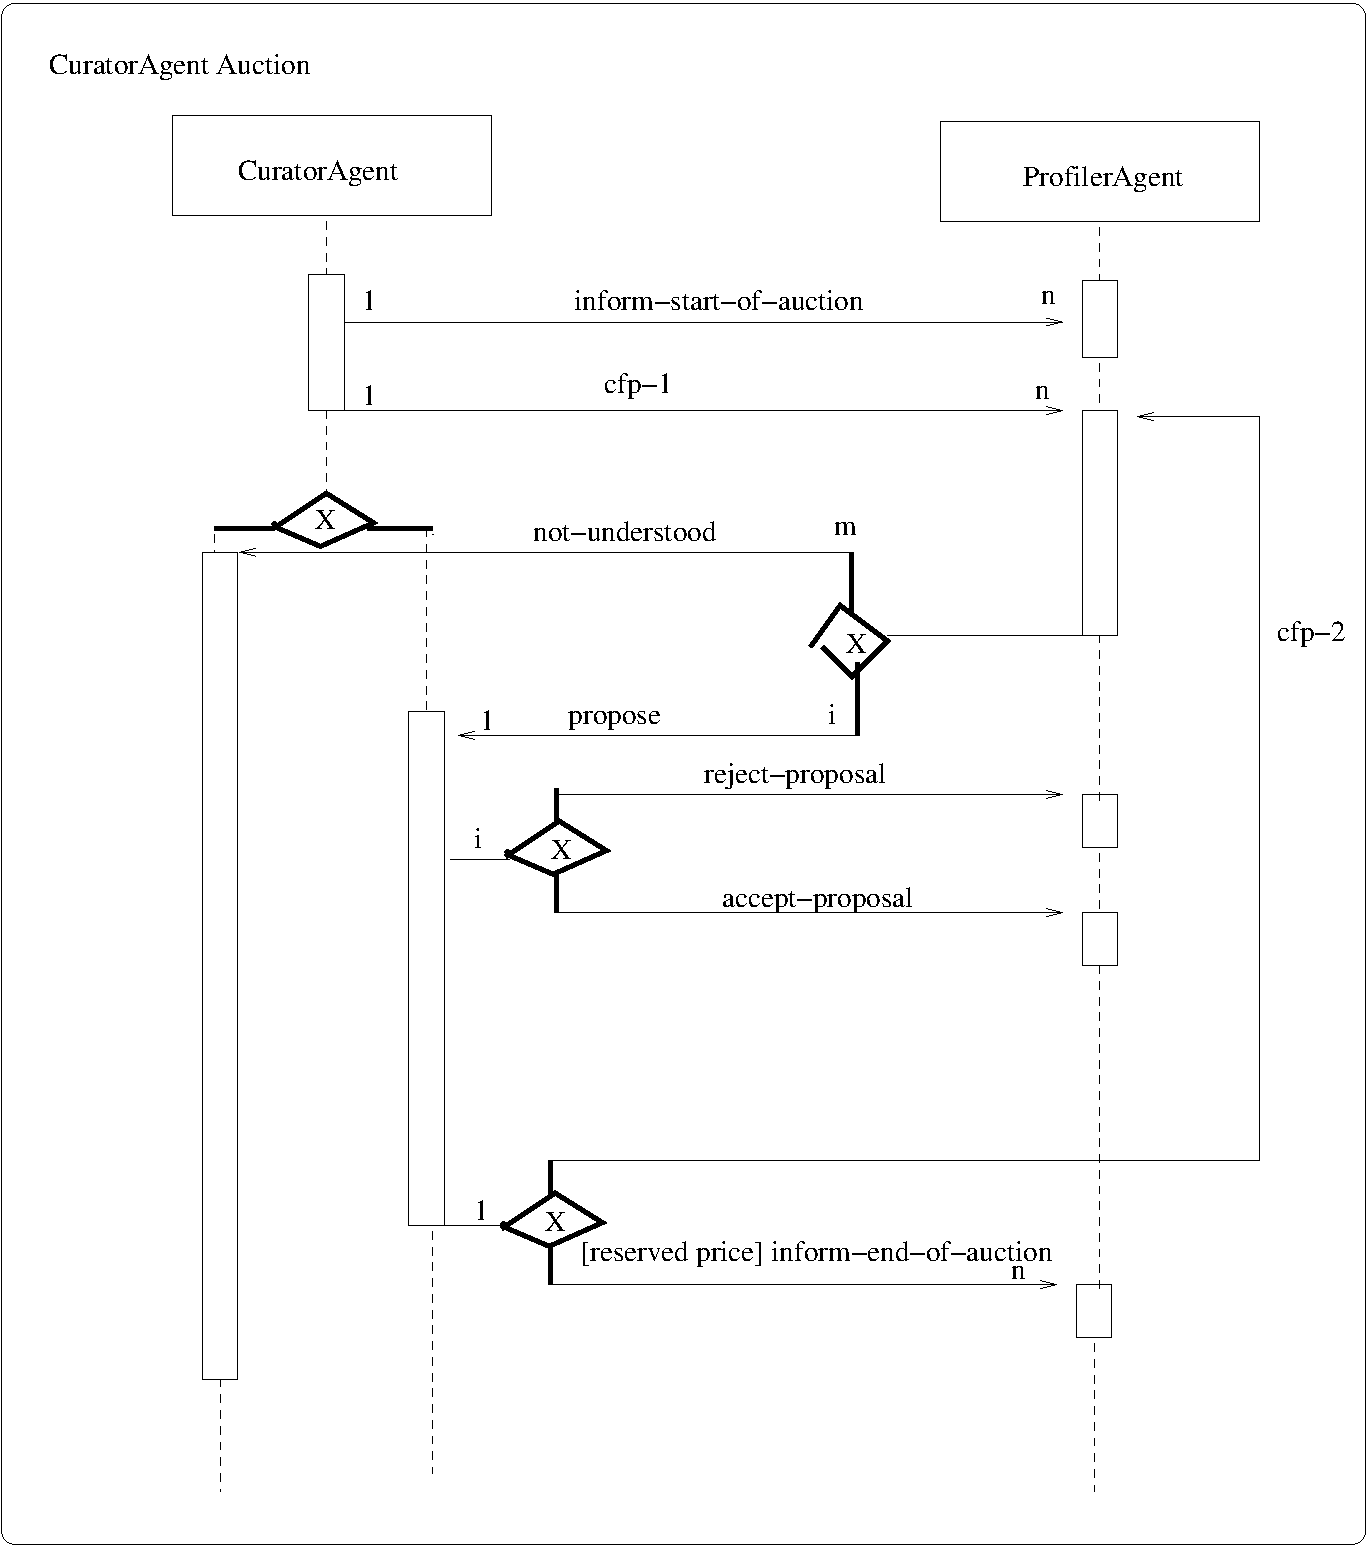
\includegraphics{curator_auction_sequence.pdf}
    }
    \caption{Sequence diagram over the interaction for CuratorAgent Auction}
    \label{fig:curator_auction_sequence}
  \end{center}
\end{figure}
\subsubsection{BuildVirtualTour}
Sequence diagram over the BuildVirtualTour protocol. When invoked the TourGuideAgent sends a $call-for-artifact-lists$ to $n$ CuratorAgents. CuratorAgents can then choose to not respond or respond with either $not-understood$ or $artifact-list-response$.
\begin{figure}[H]
  \begin{center}
    \scalebox{0.70}{
      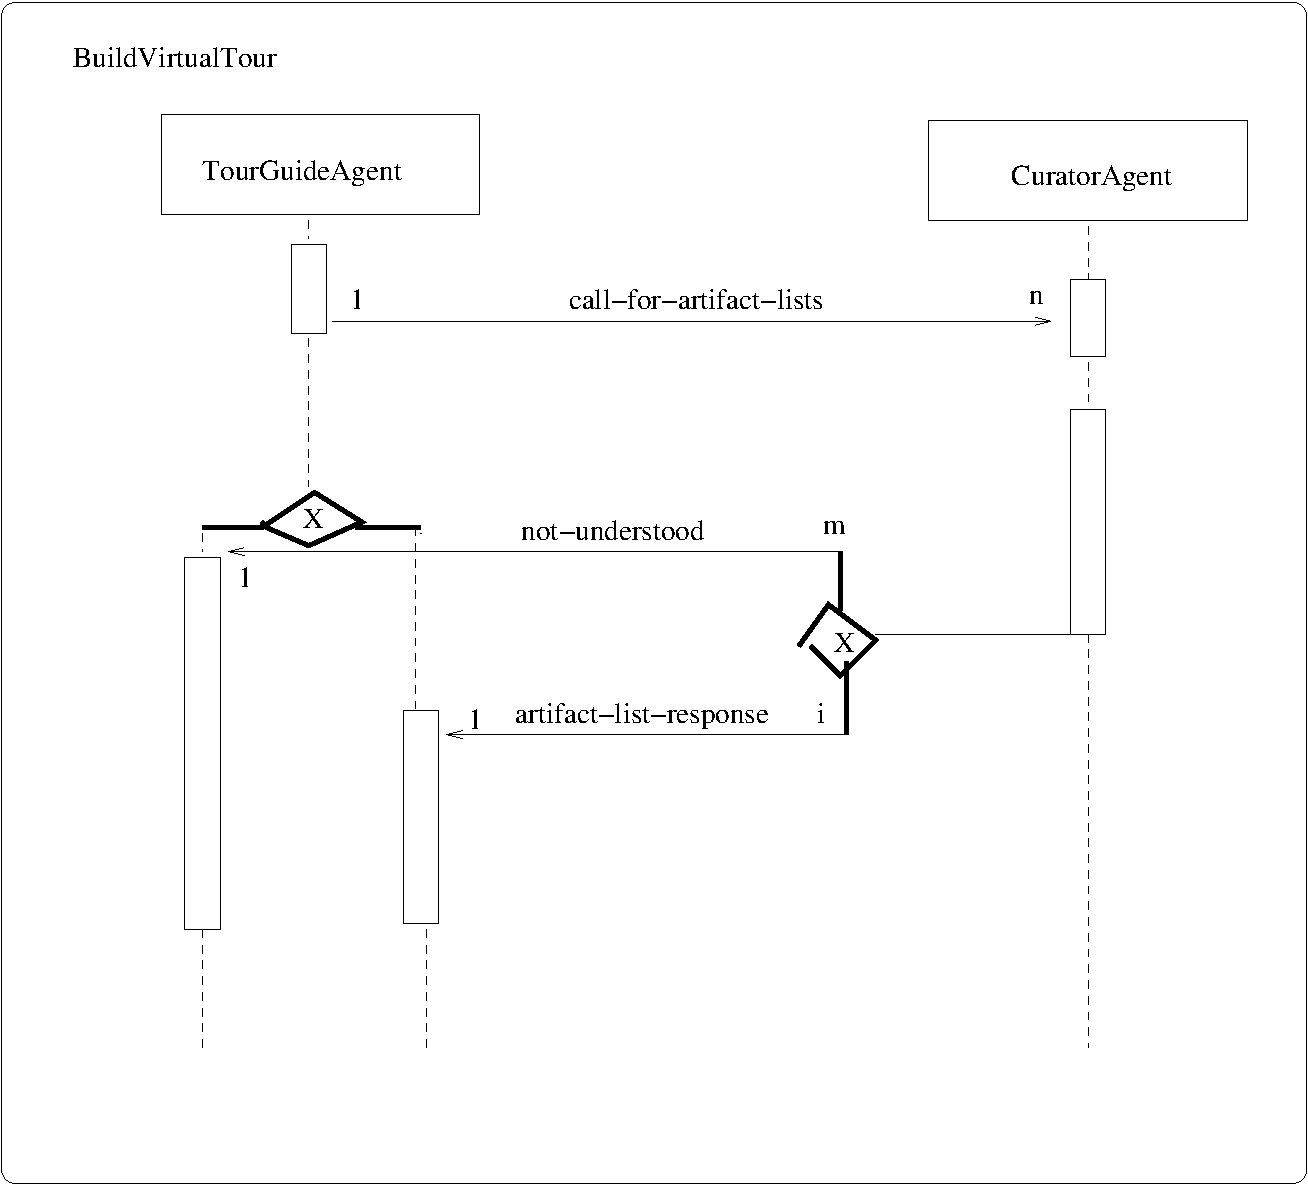
\includegraphics{build_virtual_tour.pdf}
    }
    \caption{Sequence diagram over the interaction for BuildVirtualTour}
    \label{fig:build_virtual_tour_sequence}
  \end{center}
\end{figure}
\subsubsection{FindVirtualTour}
Sequence diagram over the FindVirtualTour protocol. When invoked the ProfilerAgent sends a $call-for-available-virtual-tours$ to $n$ TourGuideAgents. TourGuideAgents can then choose to not respond or respond with either $not-understood$ or $virtual-tour-response$. If the ProfilerAgent receives a $not-understood$ message it does nothing, if it receives a $virtual-tour-response$ it either responds with $select-virtual-tour$ upon the tourguide responds with the full virtual-tour, or $reject-virtual-tour$.
\begin{figure}[H]
  \begin{center}
    \scalebox{0.70}{
      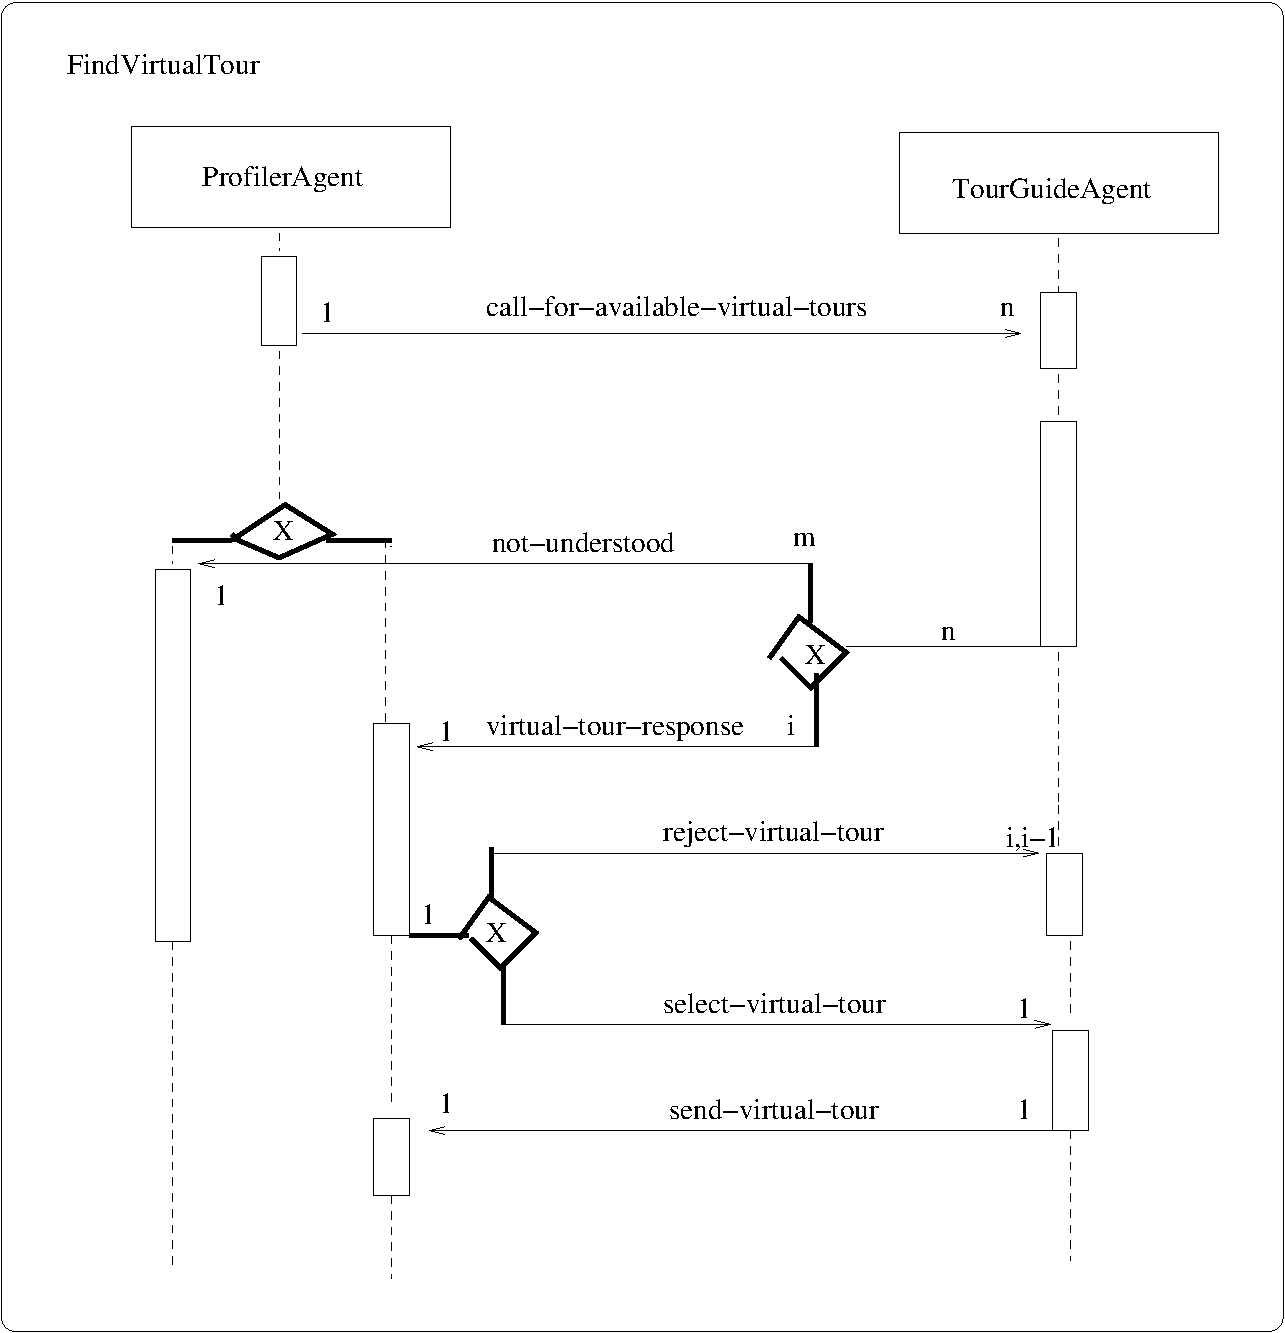
\includegraphics{find_virtual_tour_sequence.pdf}
    }
    \caption{Sequence diagram over the interaction for FindVirtualTour}
    \label{fig:find_virtual_tour_sequence}
  \end{center}
\end{figure}
\subsubsection{VisitArtifact}
Sequence diagram over the VisitArtifact protocol. When invoked the ProfilerAgent sends a $get-artifact$ message to $1$ CuratorAgent. The CuratorAgent can then choose to not respond or respond with either $not-understood$ or $artifact-response$.
\begin{figure}[H]
  \begin{center}
    \scalebox{0.70}{
      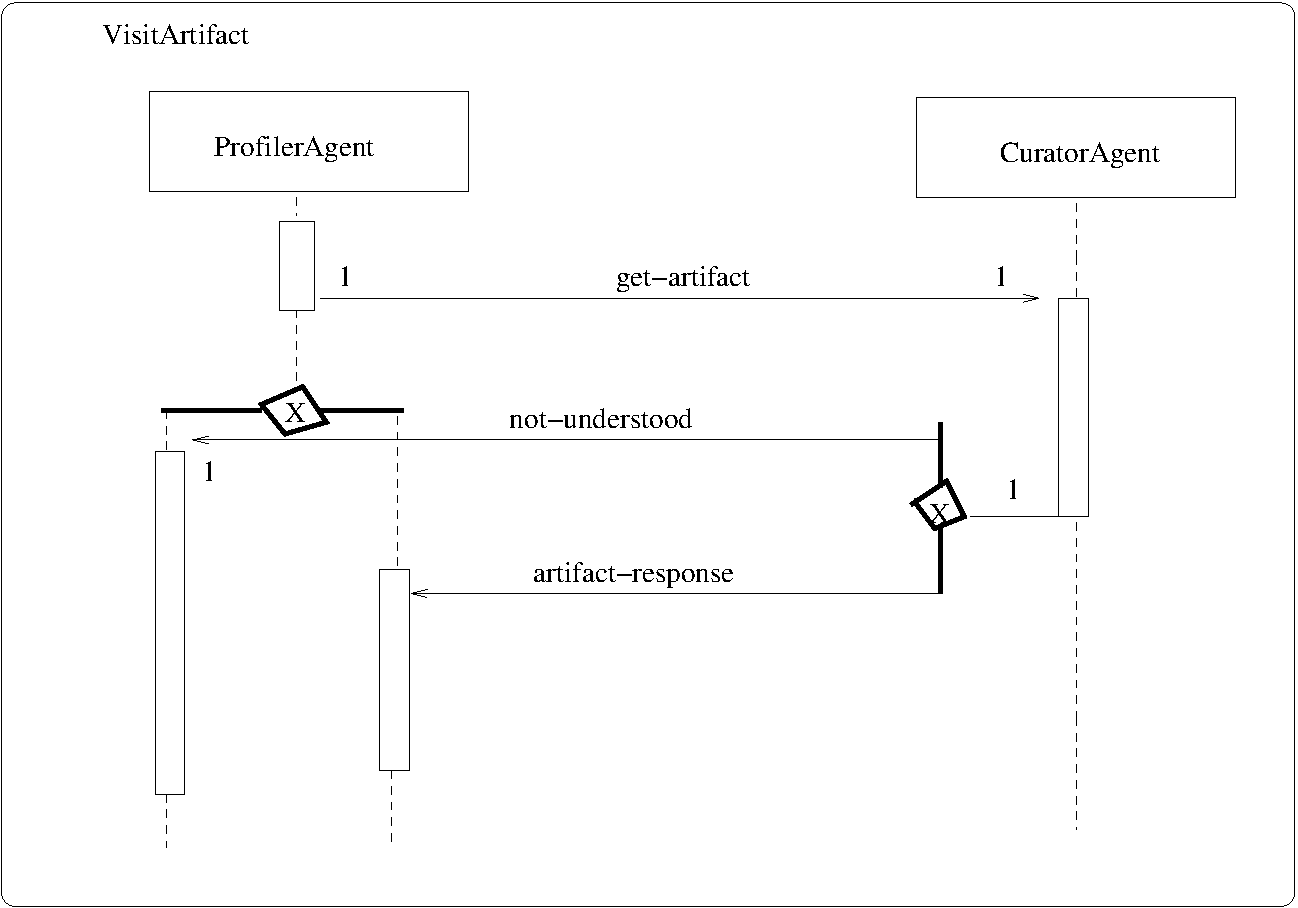
\includegraphics{visit_artifact_sequence.pdf}
    }
    \caption{Sequence diagram over the interaction for VisitArtifact}
    \label{fig:visit_artifact_sequence}
  \end{center}
\end{figure}
\subsection{Internal Agent Processing}
\subsubsection{ArtistManagerAgent}
The ArtistManagerAgent contains internal processing for modifying prices in the dutch auction as well as selecting a winner when there is multiple bids. Many of the internal states depends on external events from the interaction protocol.
\begin{figure}[H]
  \begin{center}
    \scalebox{0.70}{
      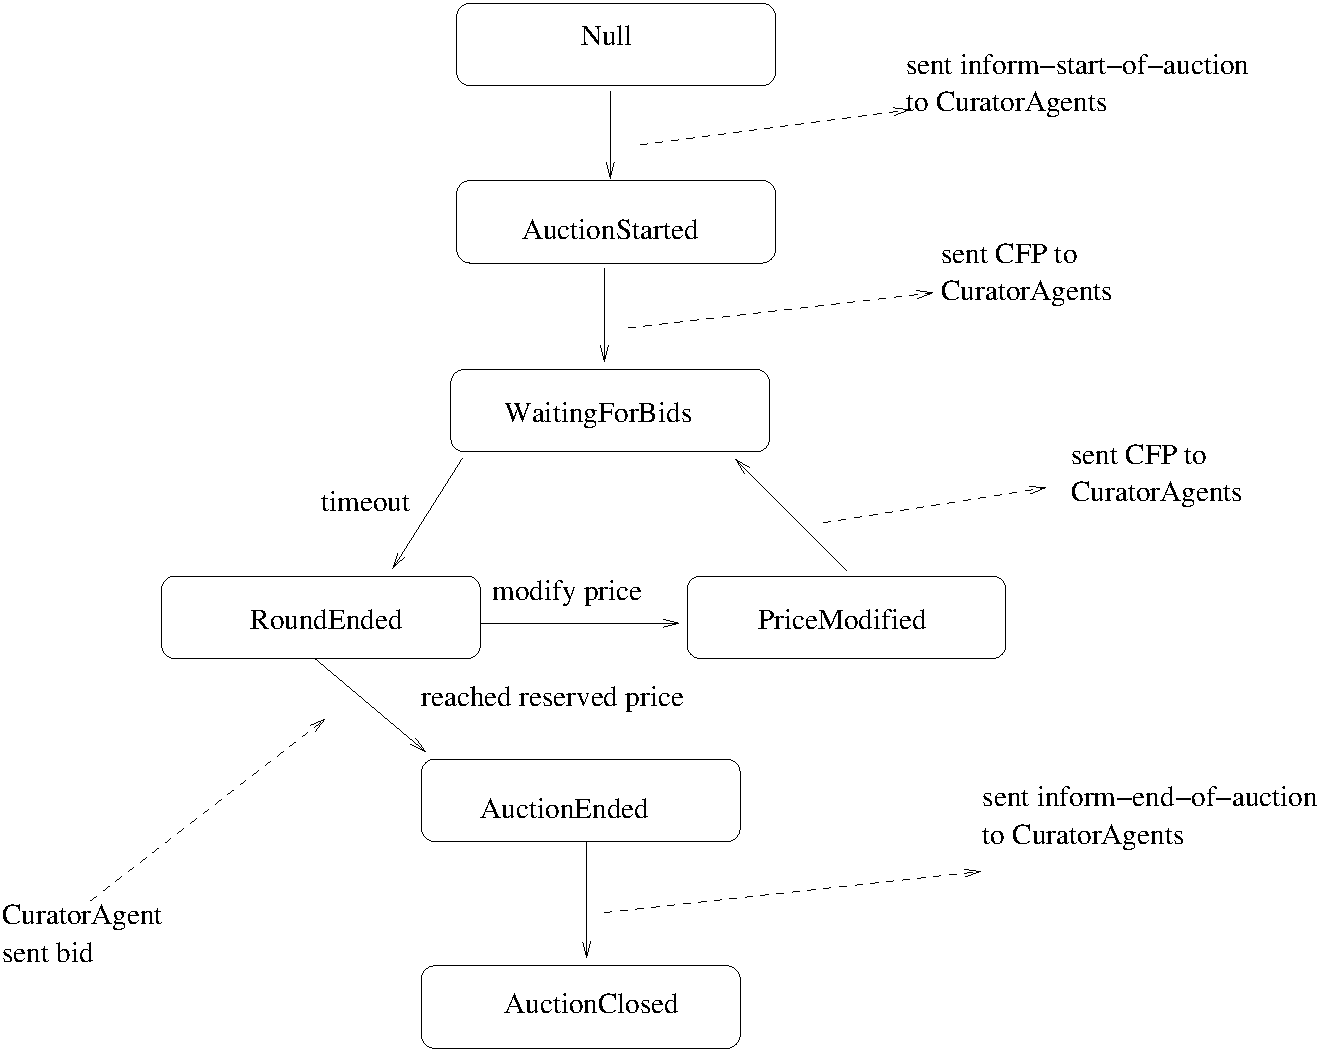
\includegraphics{artistmanager_state.pdf}
    }
    \caption{Statechart diagram for ArtistManagerAgent}
    \label{fig:artistmanager_state}
  \end{center}
\end{figure}
\subsubsection{TourGuideAgent}
The TourGuideAgent contains internal processing for building virtual tours bases on artifacts. Many of the internal states depends on external events from the interaction protocol.
\begin{figure}[H]
  \begin{center}
    \scalebox{0.70}{
      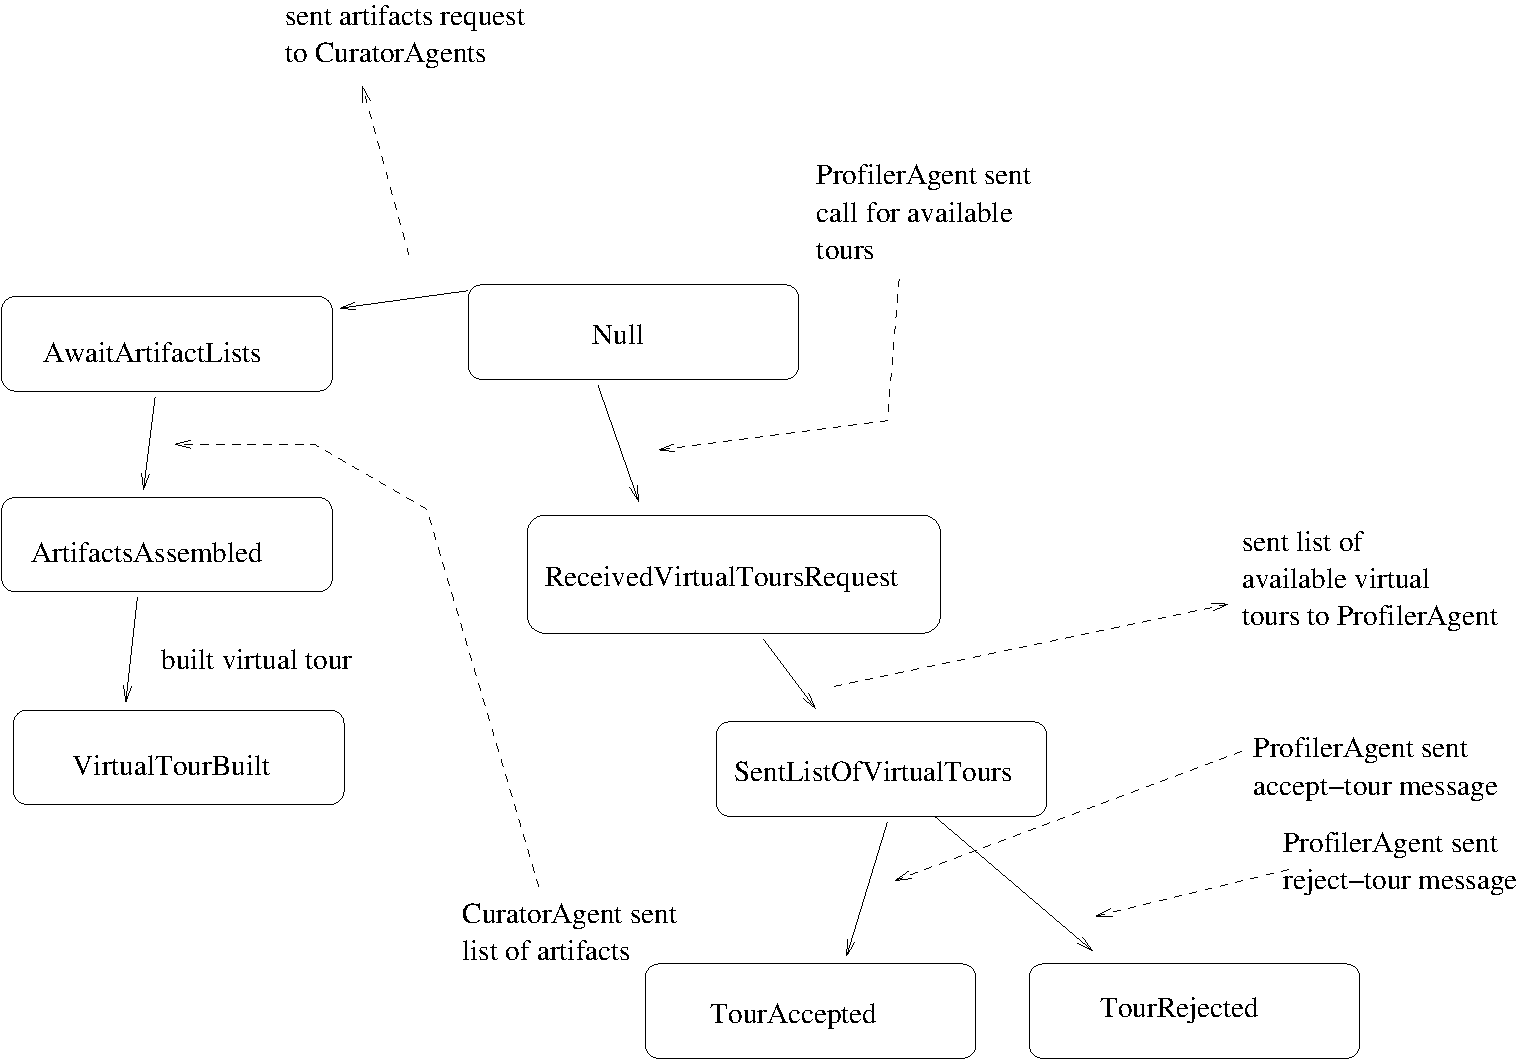
\includegraphics{tourguide_state.pdf}
    }
    \caption{Statechart diagram for TourGuideAgent}
    \label{fig:tourguide_state}
  \end{center}
\end{figure}
\subsubsection{ProfilerAgent}
The ProfilerAgent contains internal processing for choosing to participate in auctions, find virtual tours, as well as visiting artifacts. Many of the internal states depends on external events from the interaction protocol.
\begin{figure}[H]
  \begin{center}
    \scalebox{0.70}{
      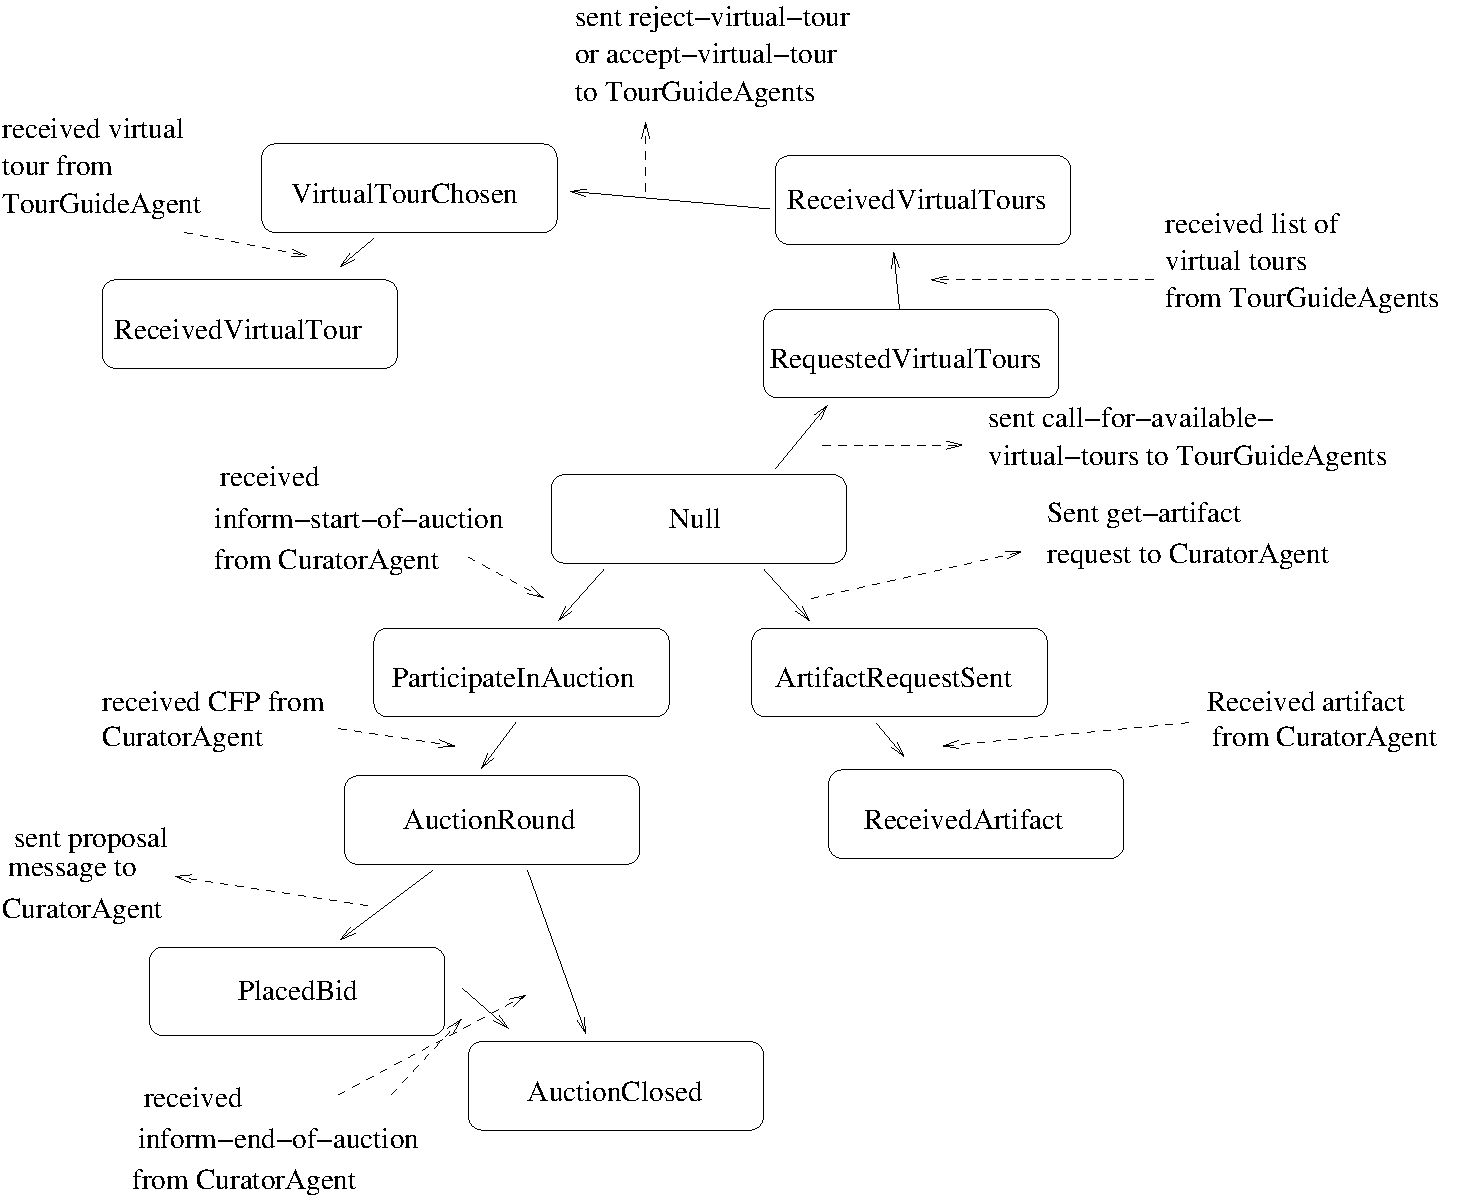
\includegraphics{profiler_state.pdf}
    }
    \caption{Statechart diagram for ProfilerAgent}
    \label{fig:profiler_state}
  \end{center}
\end{figure}
\subsubsection{CuratorAgent}
The CuratorAgent contains internal processing for participating in auctions, modifying prices in the dutch auction as well as selecting a winner when there is multiple bids. Many of the internal states depends on external events from the interaction protocol.
\begin{figure}[H]
  \begin{center}
    \scalebox{1.2}{
      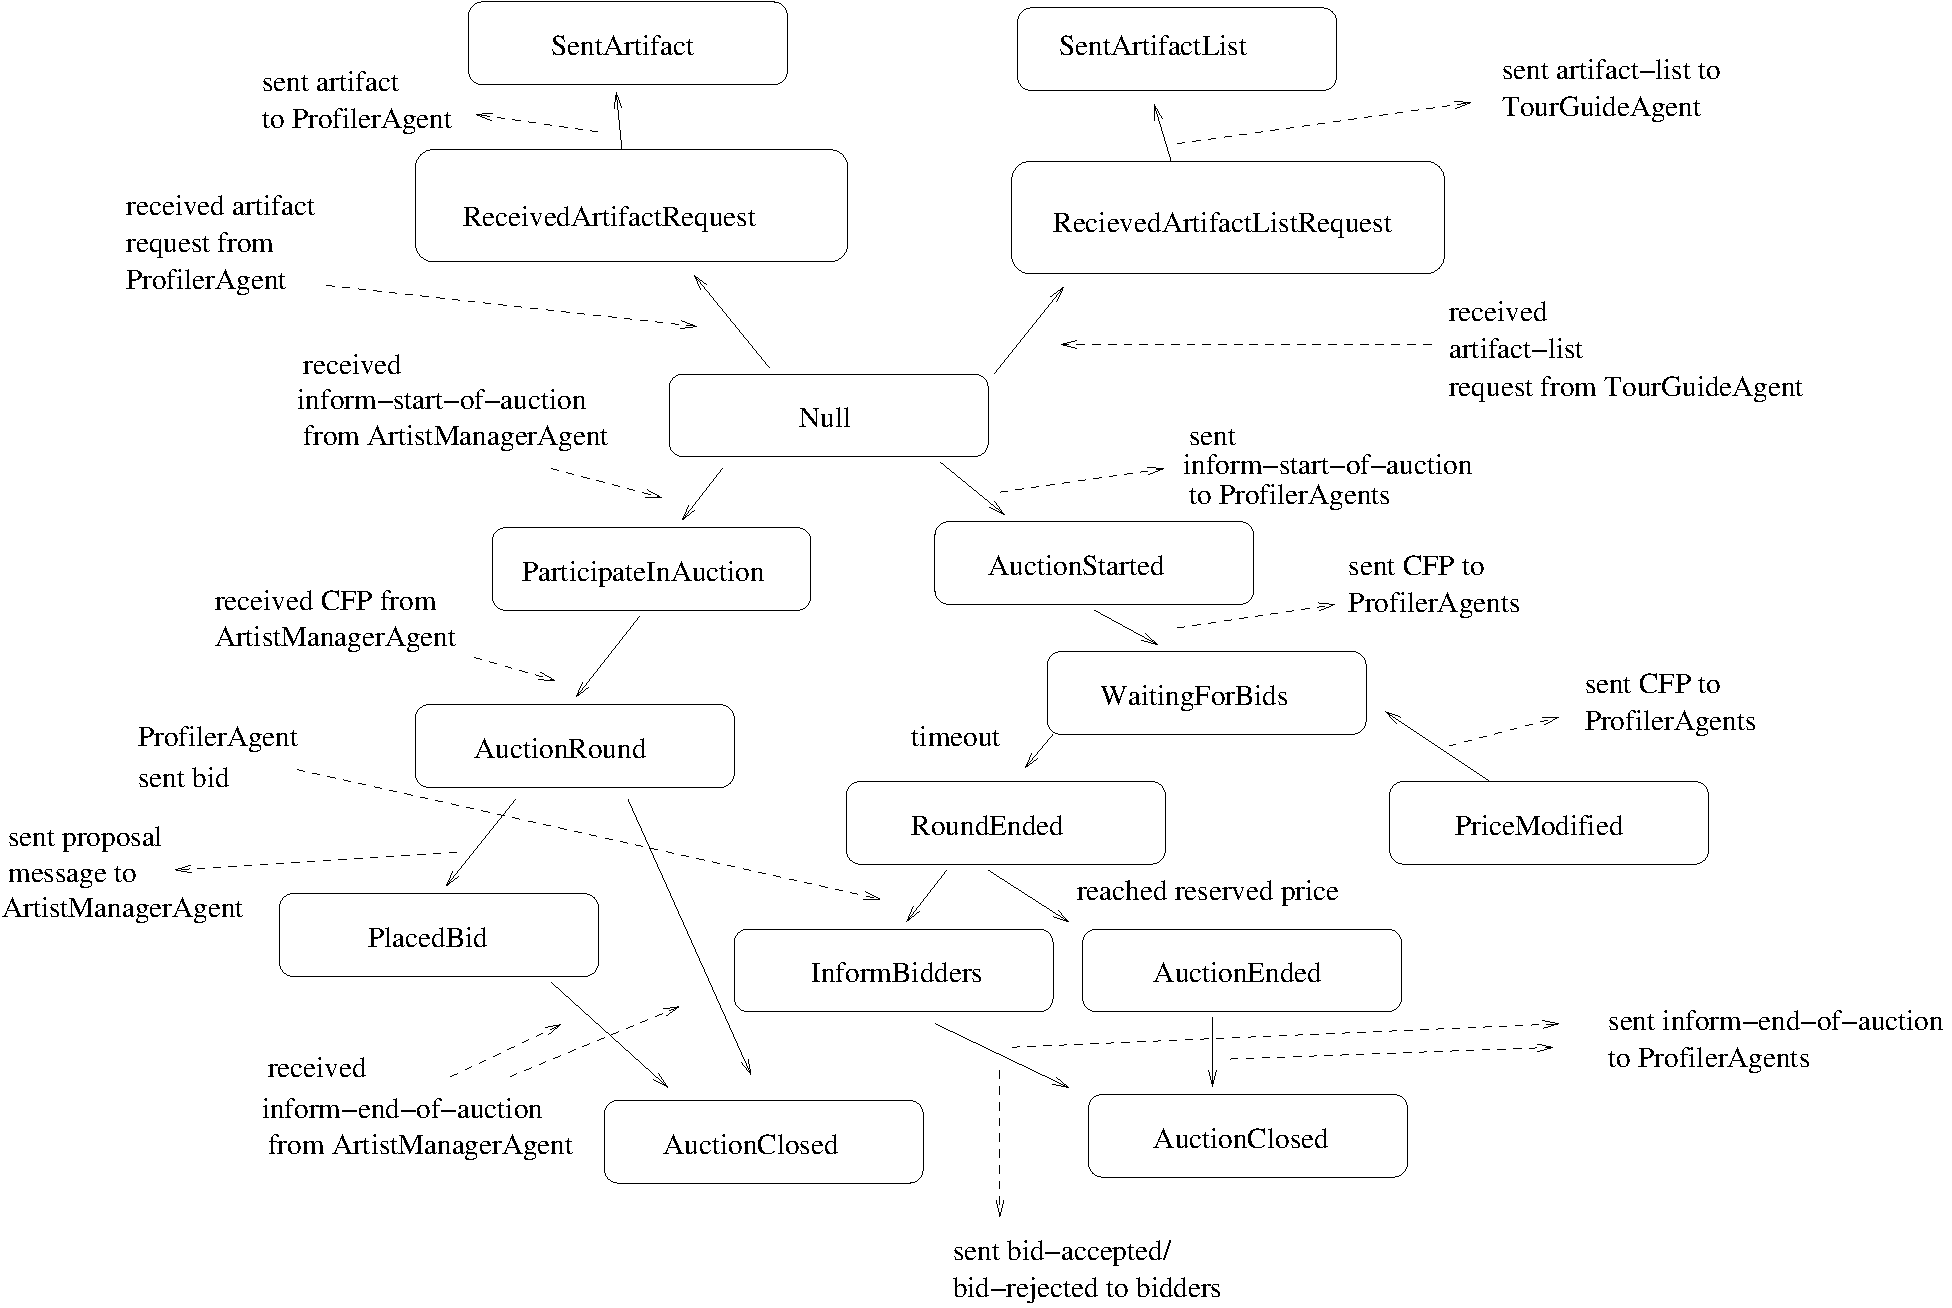
\includegraphics[width=1.0\textwidth]{curator_state.pdf}
    }
    \caption{Statechart diagram for CuratorAgent}
    \label{fig:curator_state}
  \end{center}
\end{figure}

\section{Task 3 - UML Class Diagram Revisited}
In this section the results from modelling the SmartMuseum framework with class diagrams as described in \citep{class_diagram} is presented.
\subsection{ArtistManagerAgent}
\begin{figure}[H]
  \begin{center}
    \scalebox{1.20}{
      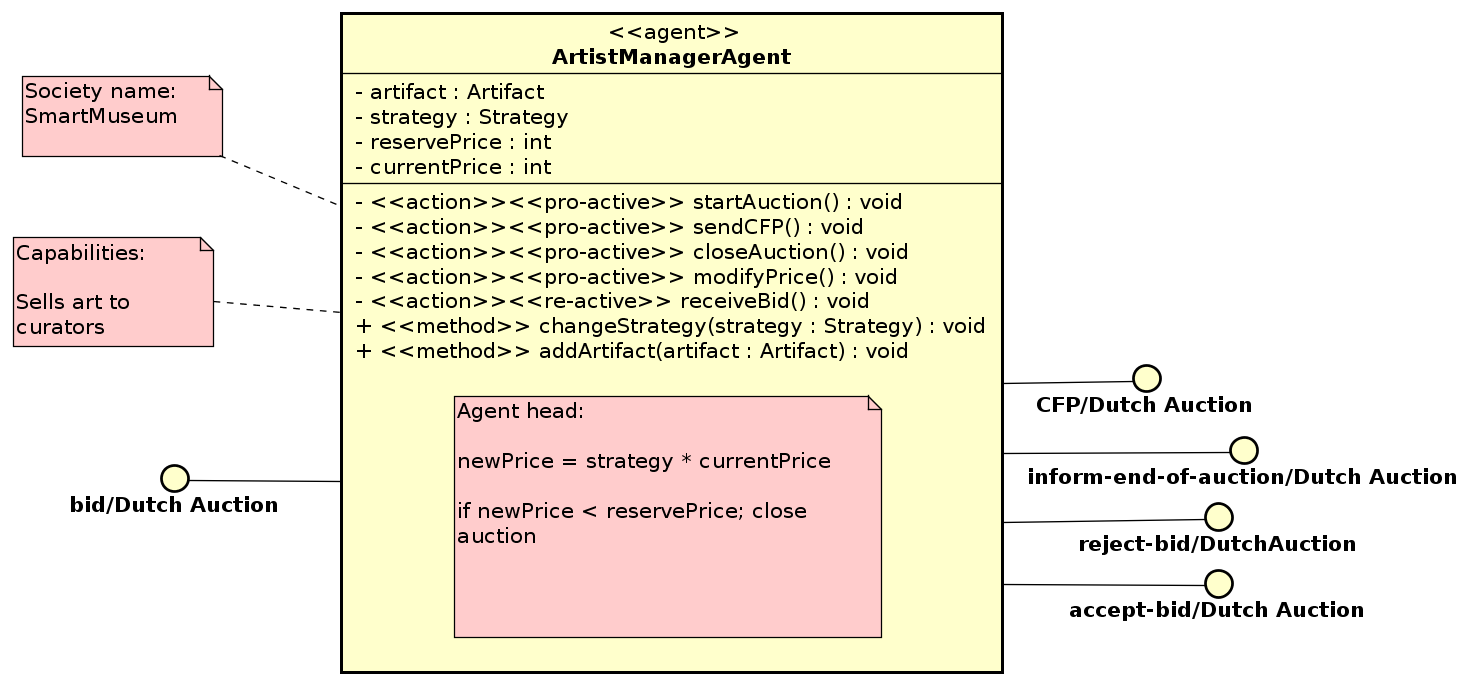
\includegraphics[width=1.0\textwidth]{artistmanager_class.png}
    }
    \caption{Class diagram for ArtistManagerAgent}
    \label{fig:artistmanager_class}
  \end{center}
\end{figure}

\subsection{TourGuideAgent}

\begin{figure}[H]
  \begin{center}
    \scalebox{1.20}{
      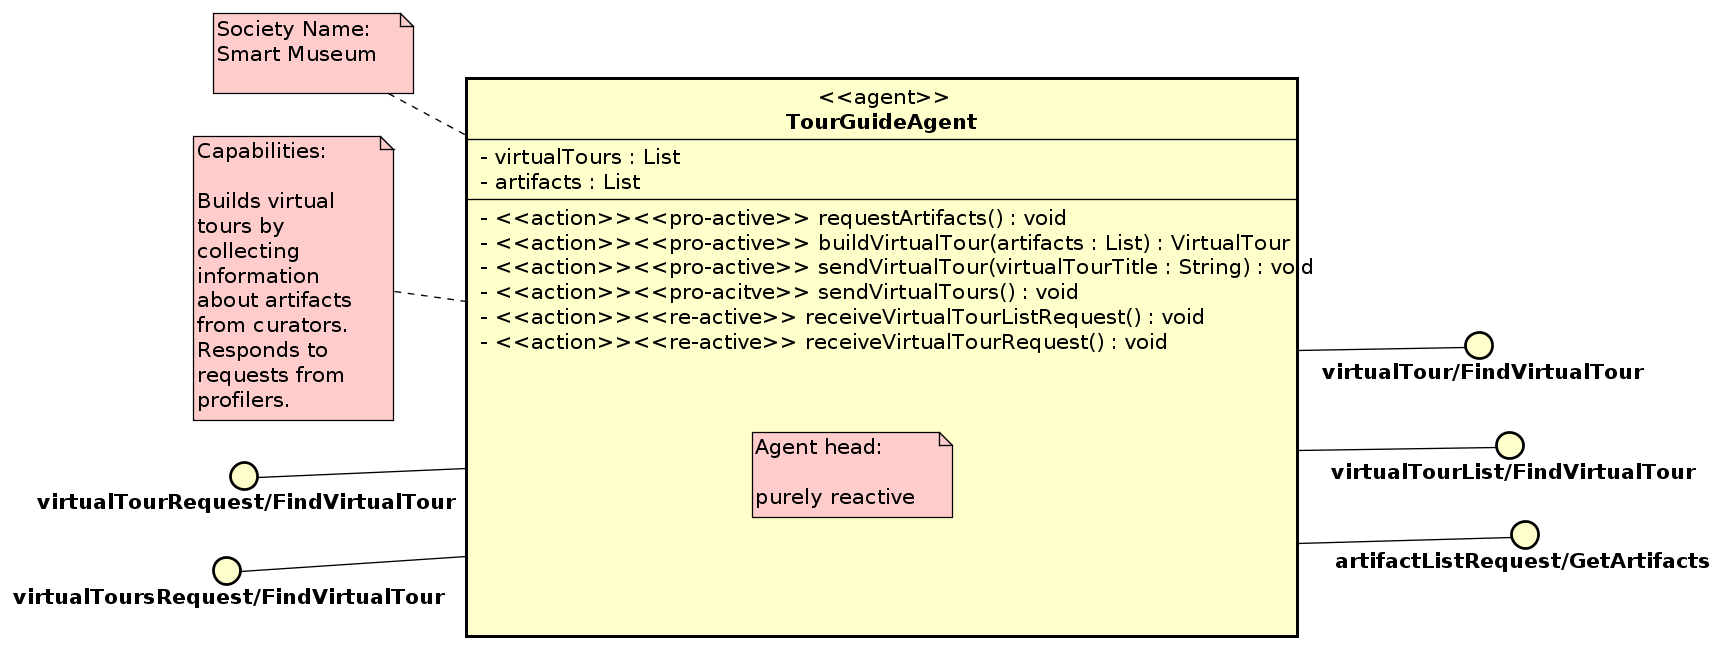
\includegraphics[width=1.0\textwidth]{tourguide_class.png}
    }
    \caption{Class diagram for TourGuideAgent}
    \label{fig:tourguide_class}
  \end{center}
\end{figure}

\subsection{ProfilerAgent}
\begin{figure}[H]
  \begin{center}
    \scalebox{1.20}{
      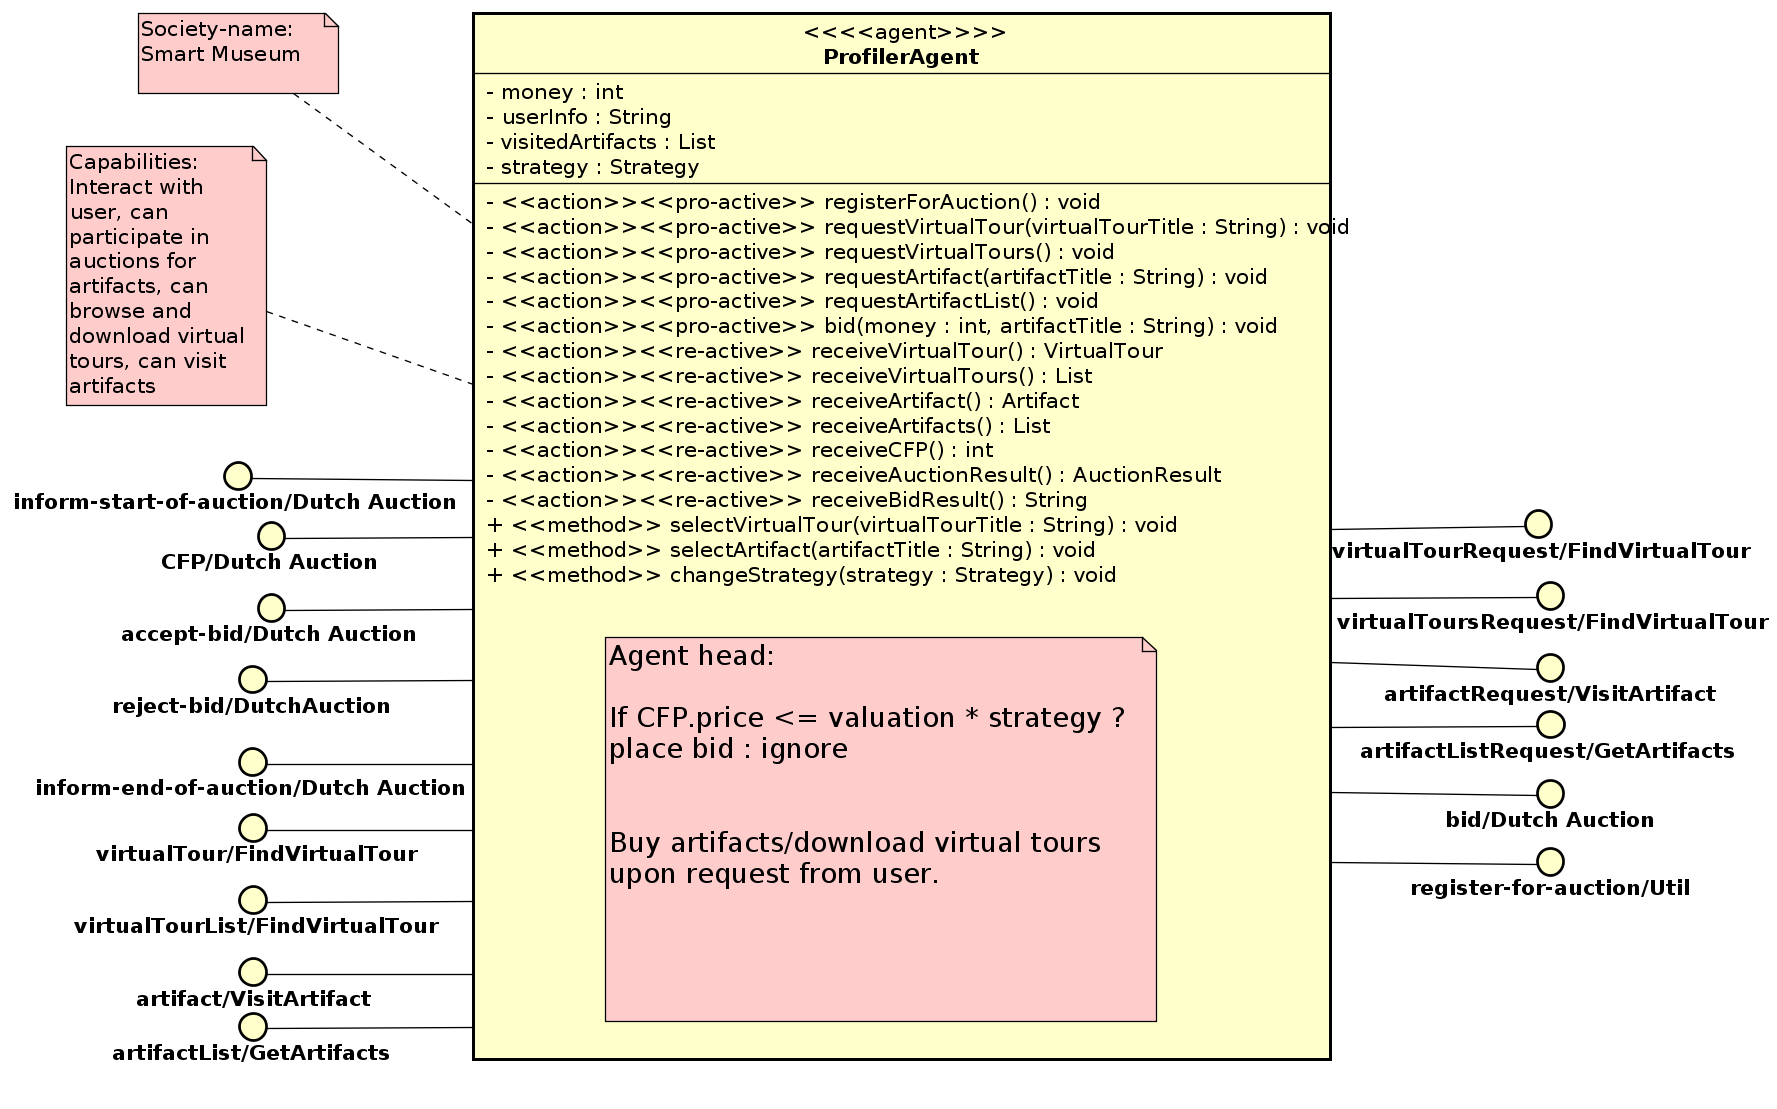
\includegraphics[width=1.0\textwidth]{profiler_class.png}
    }
    \caption{Class diagram for ProfilerAgent}
    \label{fig:profiler_class}
  \end{center}
\end{figure}
\subsection{CuratorAgent}
\begin{figure}[H]
  \begin{center}
    \scalebox{1.20}{
      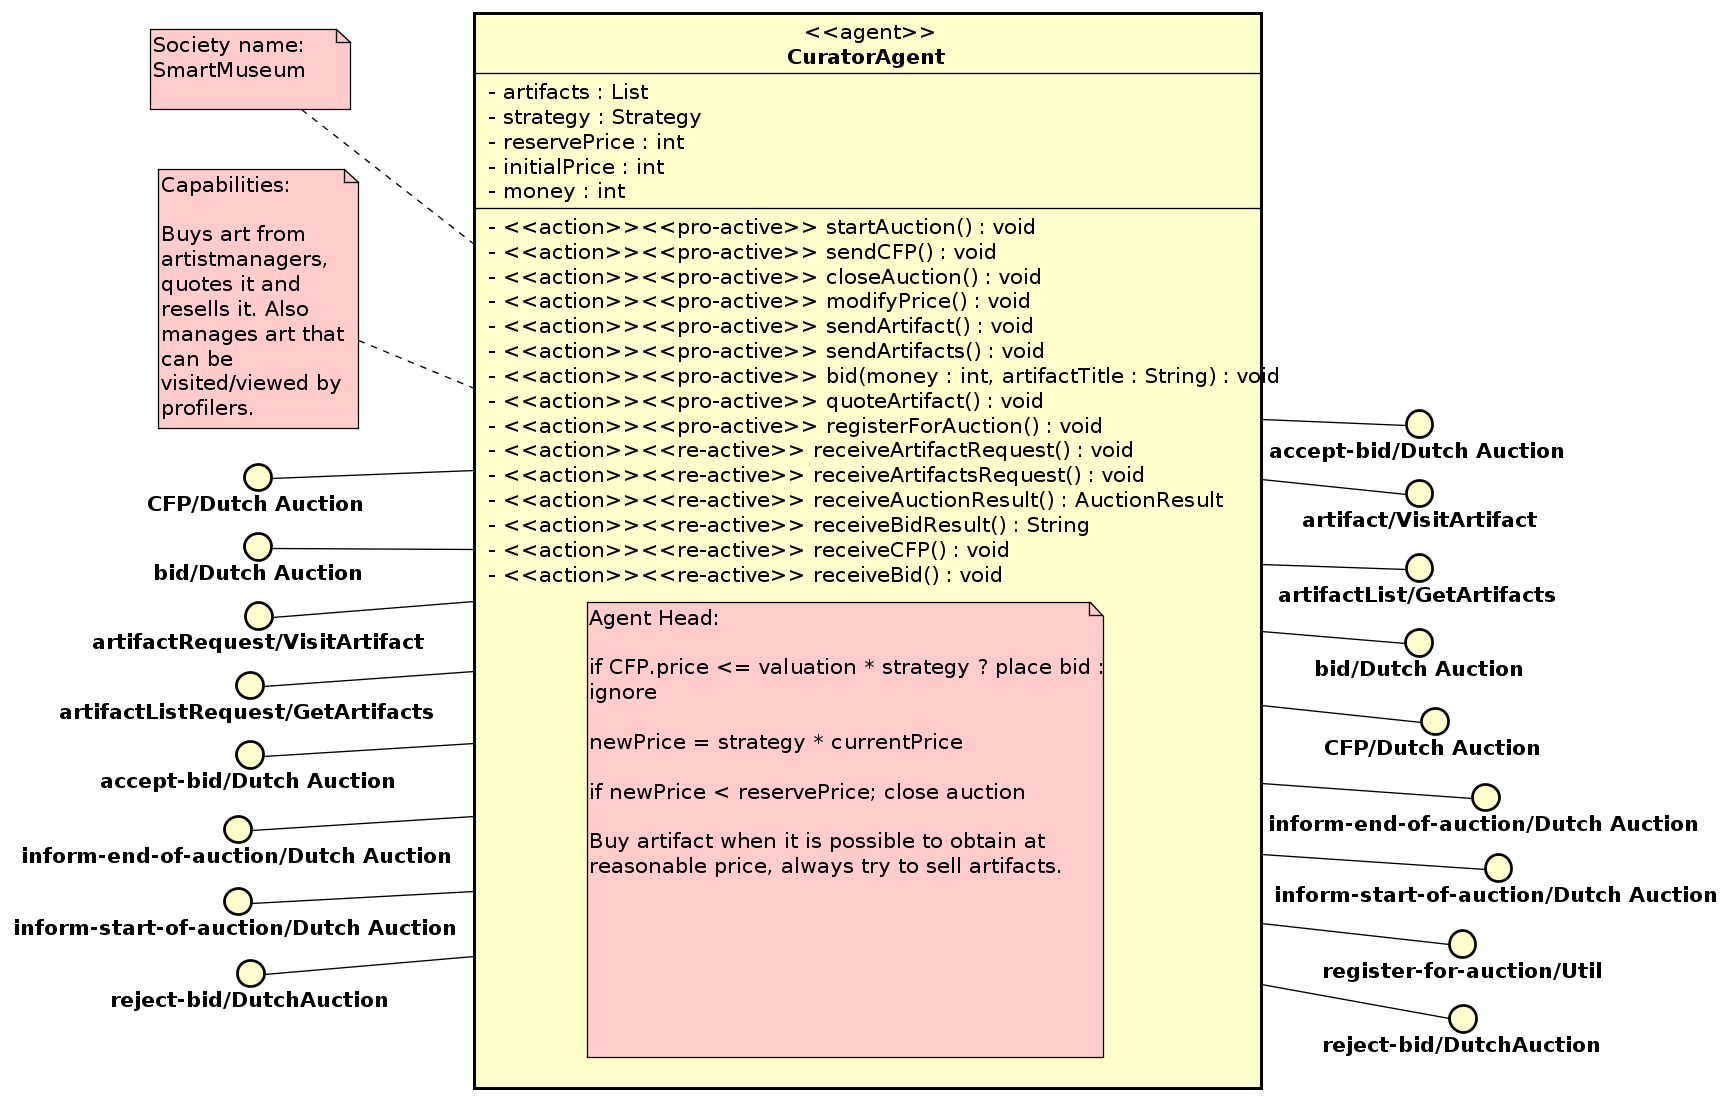
\includegraphics[width=1.0\textwidth]{curator_class.png}
    }
    \caption{Class diagram for CuratorAgent}
    \label{fig:curator_class}
  \end{center}
\end{figure}

\section{Task 4 - Role-based Modeling with RoMAS}
In this section the result from role-based modeling with the RoMAS \citep{romas} method is presented. 

RoMAS is a role-based modeling methods for agent systems, it introduces a slightly new concept of roles as compared to the role concept used in Task 1 for GAIA modeling. In particular RoMAS modeling assumes that agent and role bindings are dynamic.
\subsection{Role-based Modeling of SmartMuseum Framework}
\subsubsection{Use cases}
\begin{figure}[H]
  \begin{center}
    \scalebox{0.70}{
      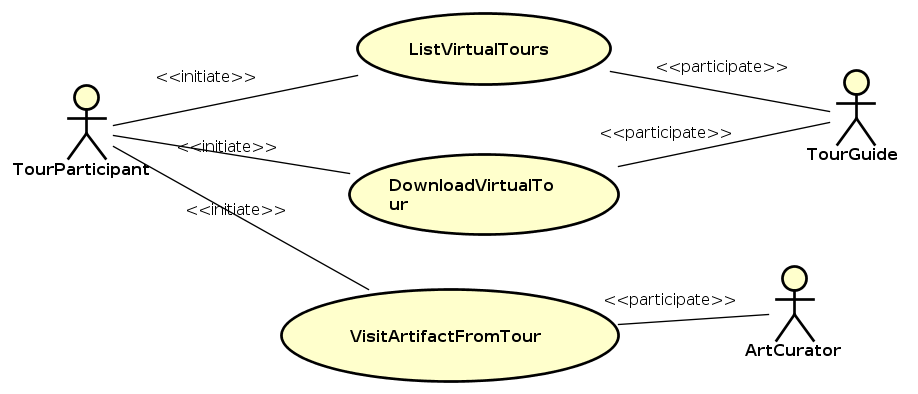
\includegraphics{consume_tour_usecase.png}
    }
    \caption{ConsumeVirtualTour usecase}
    \label{fig:consume_tour}
  \end{center}
\end{figure}
\begin{figure}[H]
  \begin{center}
    \scalebox{0.70}{
      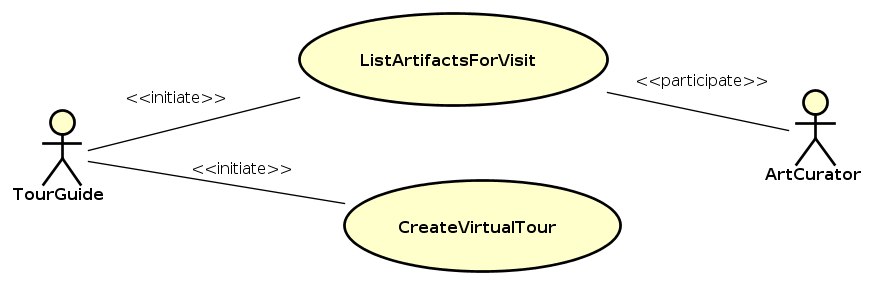
\includegraphics{create_tour_usecase.png}
    }
    \caption{CreateVirtualTour usecase}
    \label{fig:create_tour}
  \end{center}
\end{figure}
\begin{figure}[H]
  \begin{center}
    \scalebox{0.70}{
      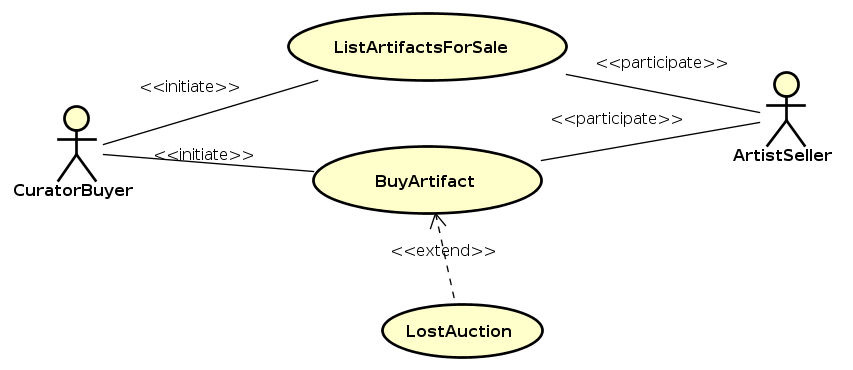
\includegraphics{curator_buy_usecase.png}
    }
    \caption{CuratorBuy usecase}
    \label{fig:curatorbuy}
  \end{center}
\end{figure}
\begin{figure}[H]
  \begin{center}
    \scalebox{0.70}{
      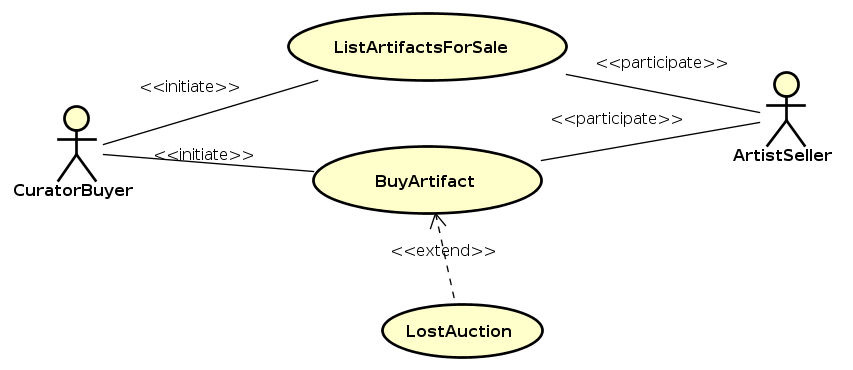
\includegraphics{hobby_buy_usecase.png}
    }
    \caption{HobbyBuy usecase}
    \label{fig:hobby_buy}
  \end{center}
\end{figure}
\subsubsection{Roles}
\begin{figure}[H]
  \begin{center}
    \scalebox{0.70}{
      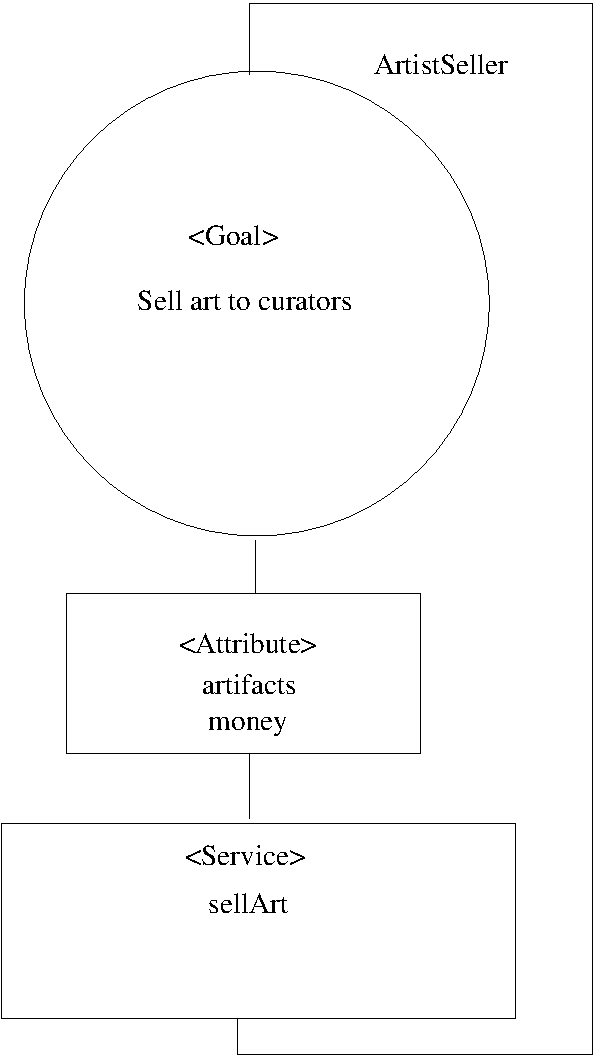
\includegraphics{artistseller_role.pdf}
    }
    \caption{ArtistSeller role}
    \label{fig:artistseller_role}
  \end{center}
\end{figure}
\begin{figure}[H]
  \begin{center}
    \scalebox{0.70}{
      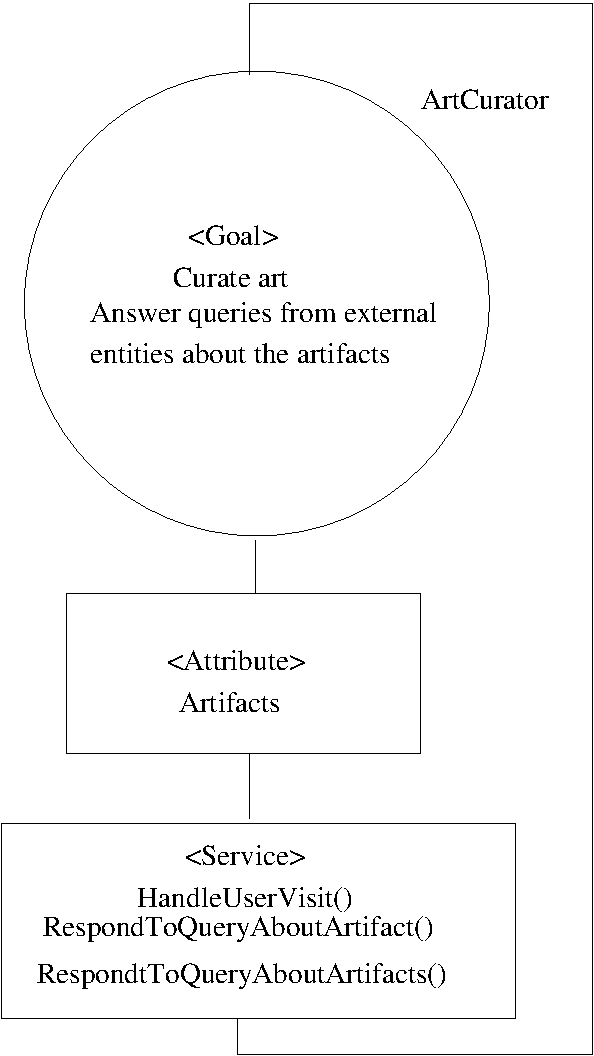
\includegraphics{artcurator_role.pdf}
    }
    \caption{ArtCurator role}
    \label{fig:artcurator_role}
  \end{center}
\end{figure}
\begin{figure}[H]
  \begin{center}
    \scalebox{0.70}{
      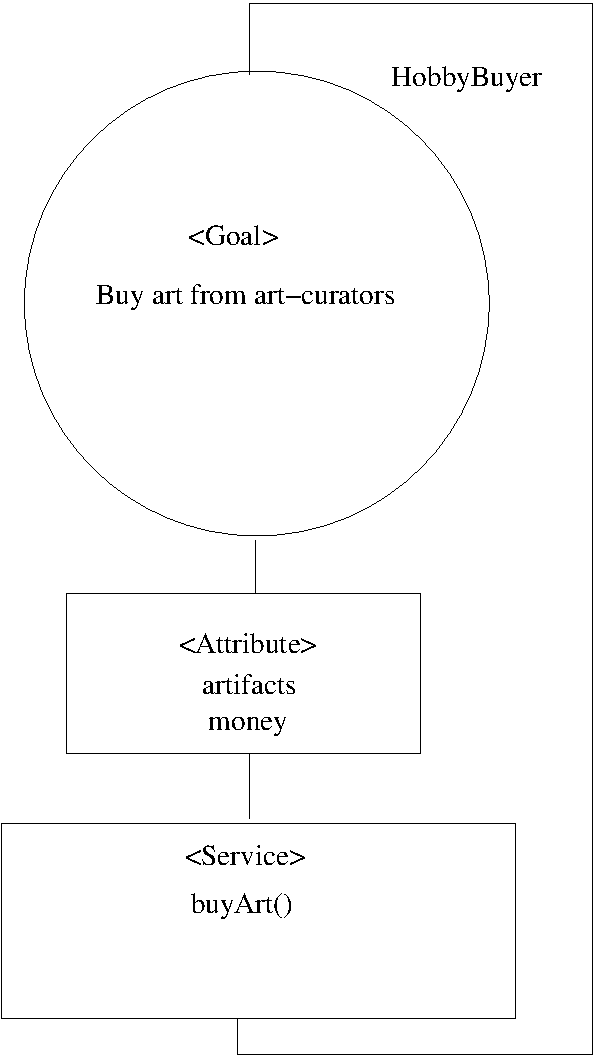
\includegraphics{hobbybuyer_role.pdf}
    }
    \caption{HobbyBuyer role}
    \label{fig:hobbybuyer_role}
  \end{center}
\end{figure}
\begin{figure}[H]
  \begin{center}
    \scalebox{0.70}{
      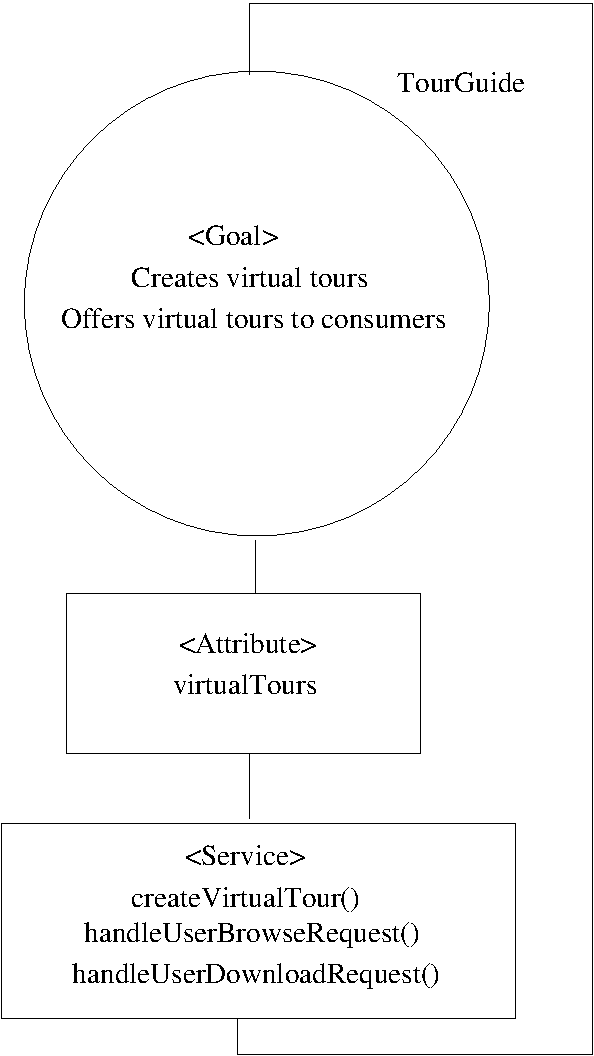
\includegraphics{tourguide_role.pdf}
    }
    \caption{TourGuide role}
    \label{fig:tourguide_role}
  \end{center}
\end{figure}
\begin{figure}[H]
  \begin{center}
    \scalebox{0.70}{
      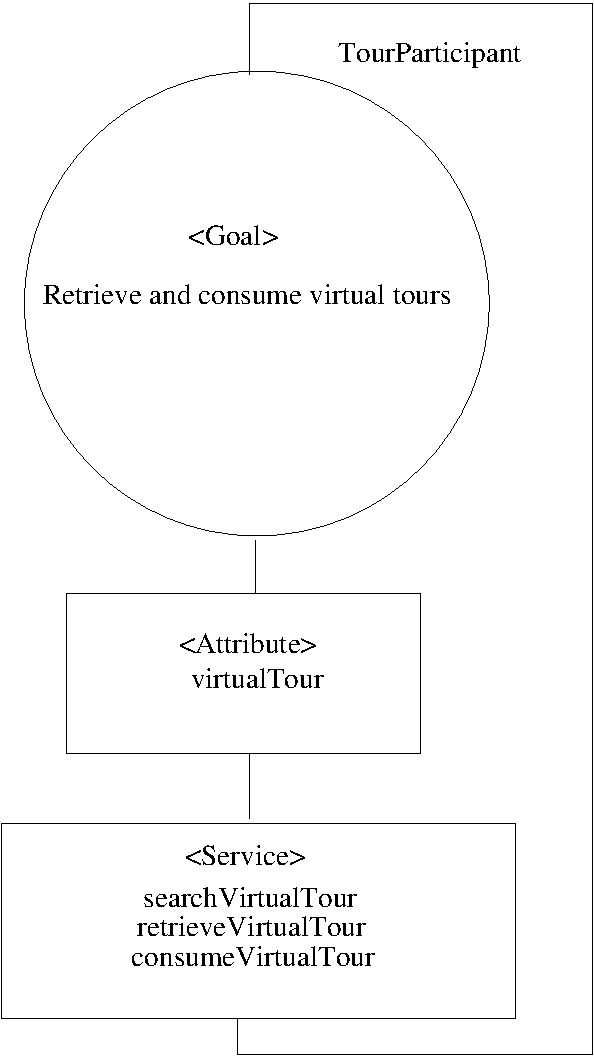
\includegraphics{tourparticipant_role.pdf}
    }
    \caption{TourParticipant role}
    \label{fig:tourparticipant_role}
  \end{center}
\end{figure}
\subsubsection{RoleOrganization}
\begin{figure}[H]
  \begin{center}
    \scalebox{1.2}{
      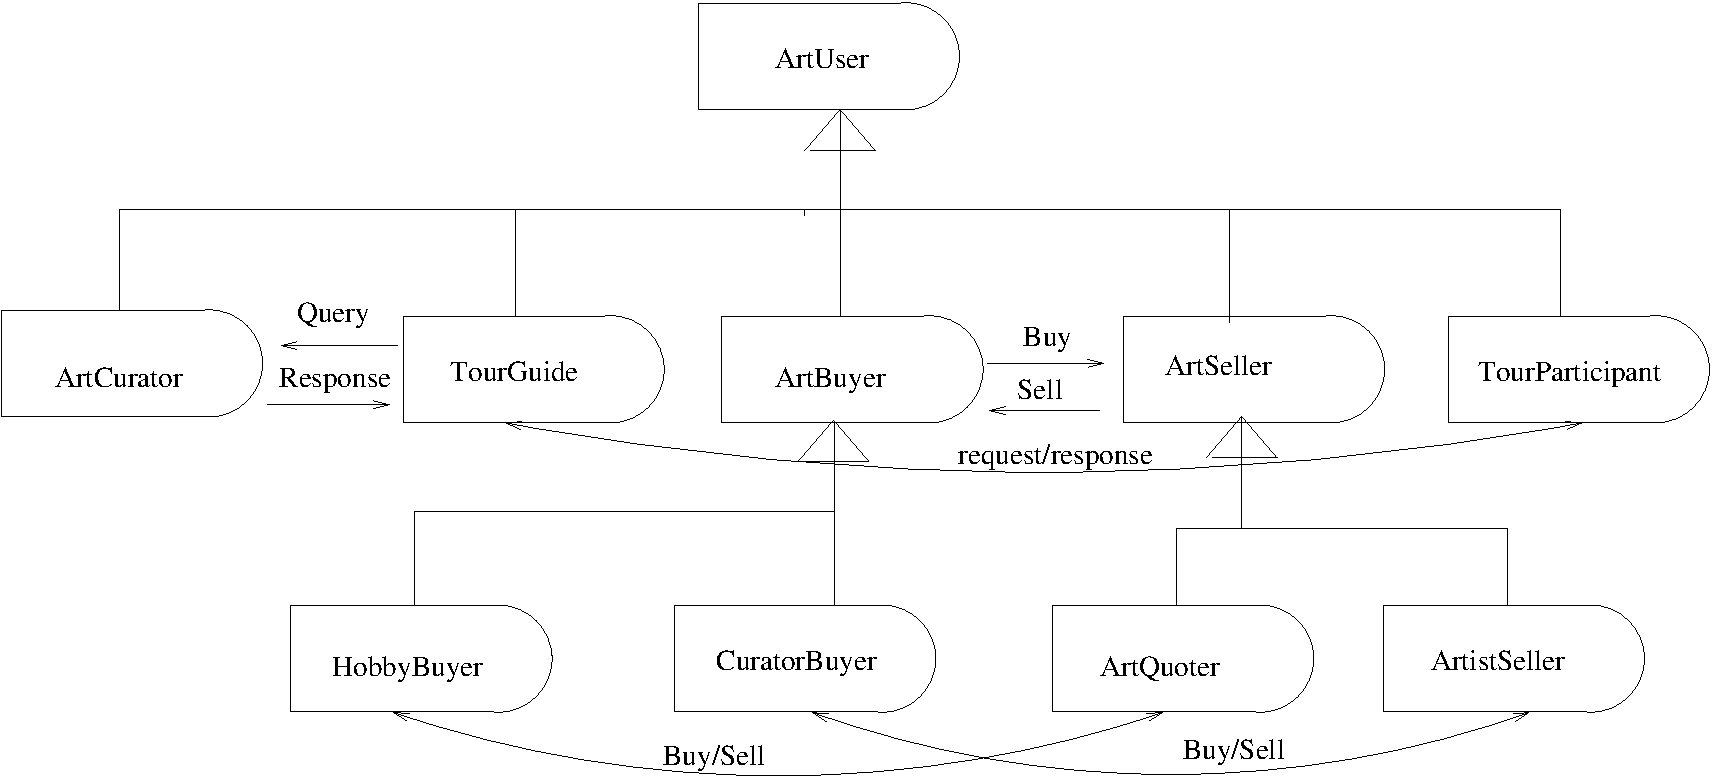
\includegraphics[width=1.0\textwidth]{roles_org.pdf}
    }
    \caption{Roles Organization}
    \label{fig:roles_org}
  \end{center}
\end{figure}
\subsubsection{Binding Agents to Roles}
\begin{figure}[H]
  \begin{center}
    \scalebox{0.70}{
      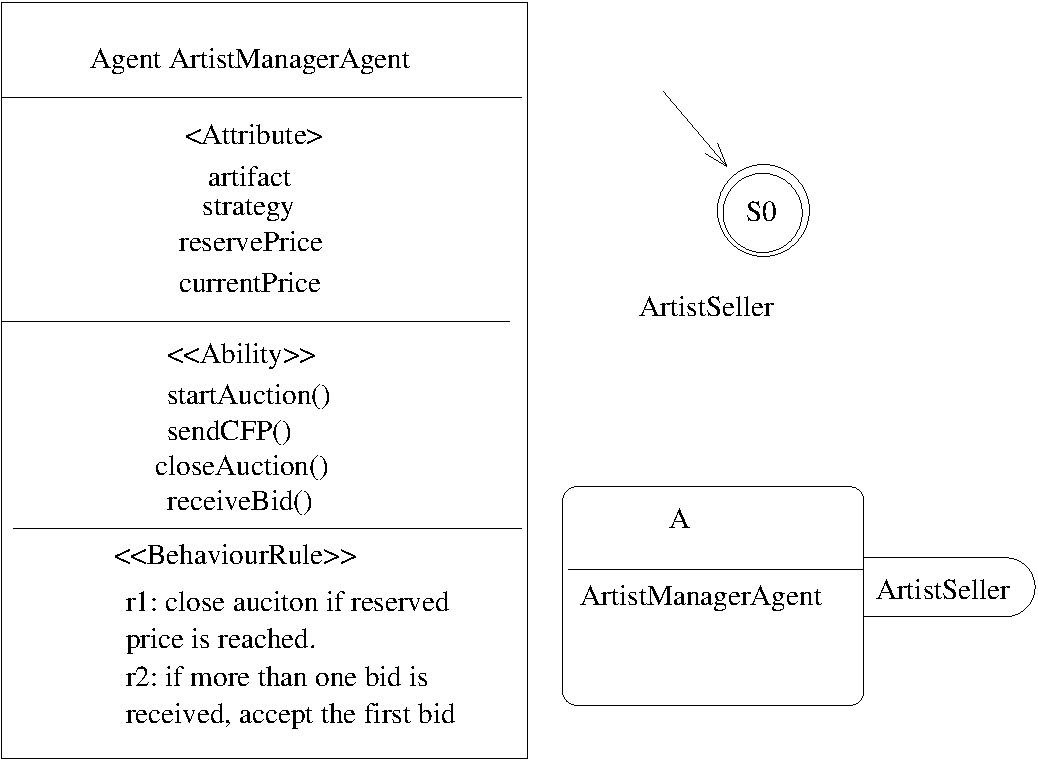
\includegraphics{artistmanager_romas.pdf}
    }
    \caption{ArtistManagerAgent binding to roles}
    \label{fig:artistmanageragent_romas}
  \end{center}
\end{figure}
\begin{figure}[H]
  \begin{center}
    \scalebox{0.70}{
      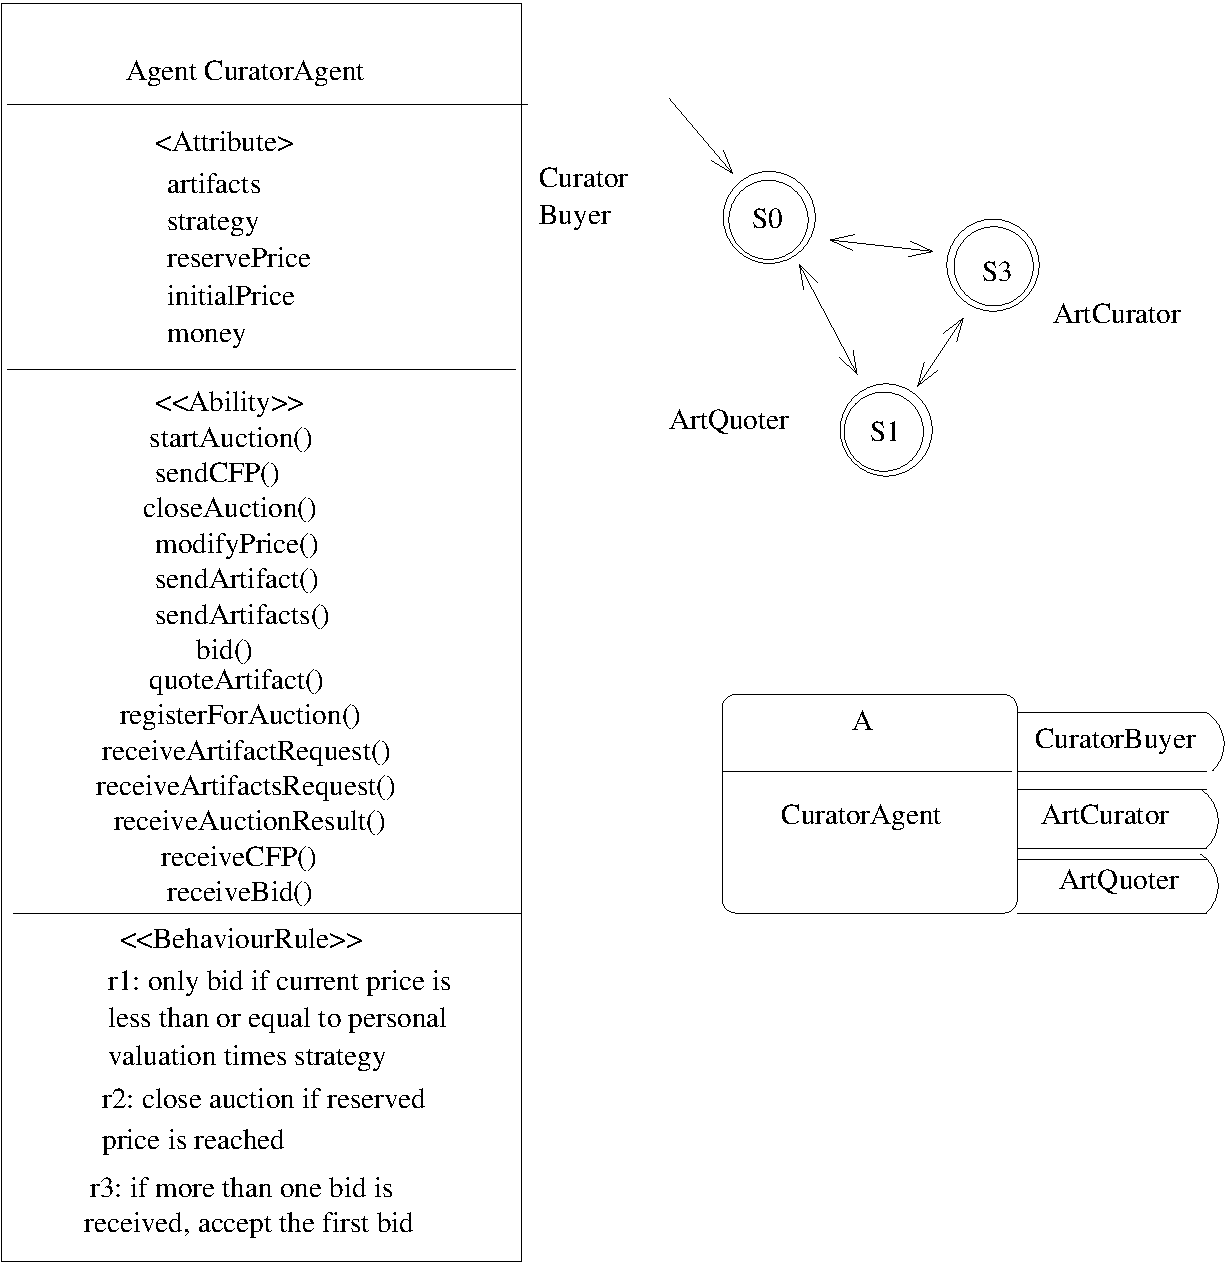
\includegraphics{curator_agent_romas.pdf}
    }
    \caption{CuratorAgent binding to roles}
    \label{fig:curatoragent_romas}
  \end{center}
\end{figure}
\begin{figure}[H]
  \begin{center}
    \scalebox{0.70}{
      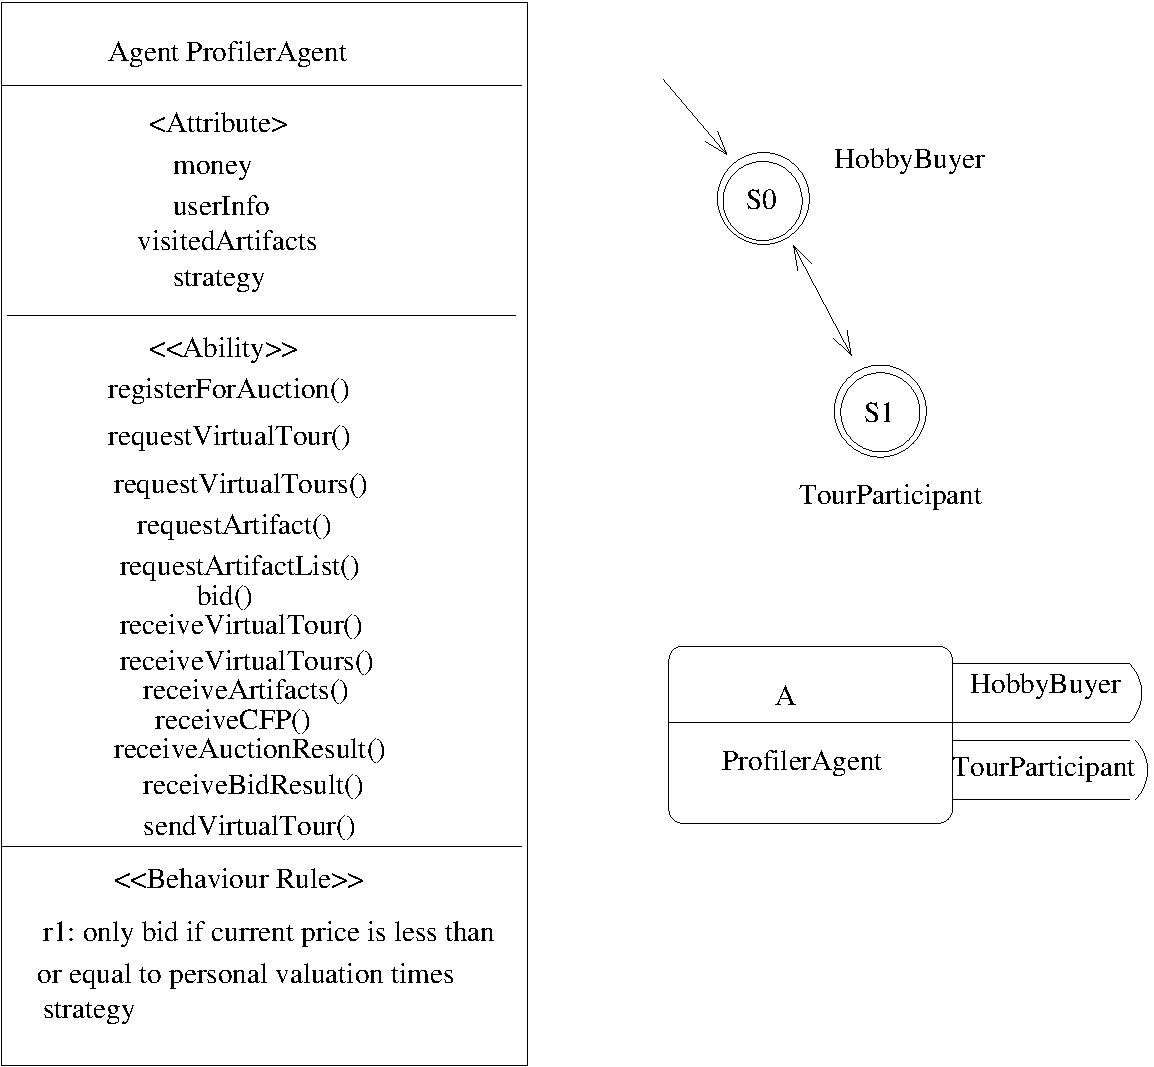
\includegraphics{profiler_agent_romas.pdf}
    }
    \caption{ProfilerAgent binding to roles}
    \label{fig:profileragent_romas}
  \end{center}
\end{figure}
\begin{figure}[H]
  \begin{center}
    \scalebox{0.70}{
      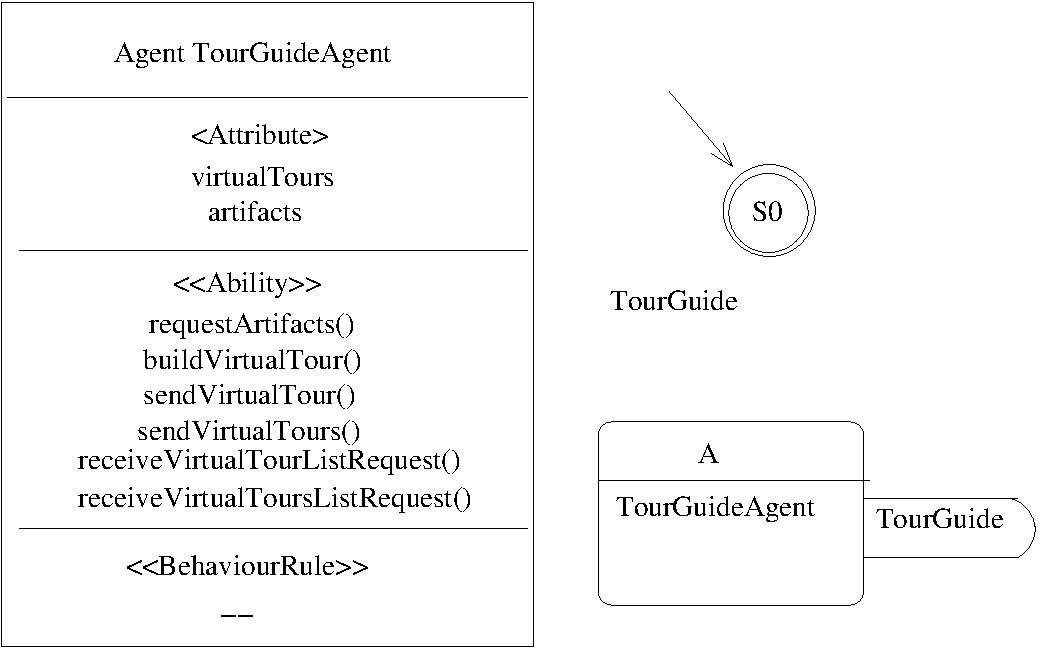
\includegraphics{tourguide_romas.pdf}
    }
    \caption{TourGuideAgent binding to roles}
    \label{fig:tourguideagent_romas}
  \end{center}
\end{figure}
\subsection{Comparison between RoMAS and GAIA}
The resulting models are very similar, the same number of roles were identified in both cases. The models differ in that with RoMAS the notion that an agent is made out of roles is very explicit while in GAIA the roles gets ``lost'' when moving into the design phase. Another disparity between the two resulting models is that in the RoMAS model the agent can dynamically change roles over time, while in GAIA the model is assumed to be static. As stated in \citep{wooldrigde_jennings}, the GAIA methdology is best suited for domains which inhabit the following characteristics:
\begin{quote}
\textit{The organisation structure of the system is static, in that inter-agent relationships do not change at run-time. The abilities of agents and the services they provide are static, in that they do not change at run-time.}\citep{wooldrigde_jennings}
\end{quote}
In constrast, the RoMAS method do support dynamic binding of role to agent at runtime, and the model only declares the \textit{initial} binding between agents and roles.
\section{Task 5 - Comparing JADE to other Agent Platforms}
In this section it follows a high-level comparison of JAVA Agent DEvelopment Framework (JADE) \citep{jade}, FIPA Open Source (FIPA-OS) \citep{fipaos}, and JACK Intelligent Agents \citep{jack}. 

JADE is a framework for developing M.A.S in java where the developer is supposed to use the regular Java language but adopt the guidelines provided by the framework to construct agent systems. JACK is an agent platform developed on top of and integrated with Java, it works as an agent-oriented extension to the object-oriented Java, it is its own language although closely coupled with java. FIPA-OS is a set of components which constitute as the core of the FIPA specification, which means that the developer can utilize this and focus on solving the real problem instead of building agent infrastructure.

\subsection{Services and Architectures}
\begin{tabular}{|p{2cm} p{6cm} p{6cm}|}
\hline
\textbf{Platform}  & \textbf{Architecture} & \textbf{Services} \\
\hline
JADE & Container-oriented architecture. Distributed containers that are connected over the network through a message transport system provided by JADE. \citep{jade-2}& Agent Management System (AMS) can kill/create agents, provides a naming service for all agents on the platform. Directory Facilitator (DF) provides a Yellow Pages service which agents can use to find each other.  \citep{jade-2}\\
\hline
FIPA-OS & Component-oriented architecture. When deploying an agent system the developer choose a set of components to use, some components are mandatory, some are optional. \citep{fipa-os-2}& Core components: Agent Shell provides a shell for agent implementation, TM (Task Manager) support ability to split functionality of agents, CM (Conversation Manager) enables to track conversation state at the performative level, MTS (Message Transport Service) the general messaging service that enables agents to communicate. Beyond the mandatory components there are a bunch of optional components, e.g database factory, parser factory. FIPA-OS also provides Directory Facilitator and Agent Management System just as JADE \citep{fipa-os-2}.\\
\hline
JACK  & JACK Agent Kernel, a runtime engine that provides the infrastructure for developing agent systems. JACK uses a communication layer. The developer is not actively interacting with the kernel but instead uses constructs in the language declaring the name of agents, the address of other agents etc, which will allow the kernel to provide the underlying infrastructure, e.g communication between agents. \citep{jack-2} & JACK provides a default messaging service over UDP and has constructs for a naming-service in the language. One particular agent architecture have stronger support than others in JACK and that is the BDI architecture. JACK provides different services related to BDI such as BDI Models, ways of declaring plans, beliefs and external/internal events. TaskManager which allows agents to schedule tasks. JACK also provides services for team-oriented programming as a way of coordinating between agents. \citep{luck_book}\\
\hline
\end{tabular}

\subsection{Implementation Comparison}
\begin{itemize}
\item \textbf{JADE}: \\
In JADE, service implementation can be done by developing agents that listens for certain type of messages, perform some action, and respond. The functionality for listening for a certain type of messages is provided by the JADE runtime and allows to have multiple services on the same host in a convenient way. Service registration and discovery is closley coupled with the AMS Service and the DF service. The AMS service ensures a global name space with unique names for adressing, the DF service is used to register services and to find other registered services. AMS and DF are agents on their own which means that the interaction with these services is done through messages passing. When registering a service one could define different properties like name, type, description etc. 
\item \textbf{FIPA-OS}: \\
Service implementation in FIPA-OS can be done by developing agents that listens for specific type of incoming connections by developing Tasks, Tasks's can then be associated to different events which allows to have multiple tasks on the same host/agent. FIPA-OS uses the same type of services like JADE for service registration and discovery: AMS and DF \citep{fipa-os-2}.
\item \textbf{JACK}: \\
In JACK an agent service can be implemented by using the constructs in the language like \texttt{\#handles} to declare which events this service/agent should react to, \texttt{\#posts}, \texttt{\#sends} for event/message sending, \texttt{\#uses} for declaring plans. To set up a service in JACK which can be used by other agents, one can use a designated process/agent as a \textit{name-server}, this name server can be designed in different ways, for example it could do lookups of names to port/address, or it could provide a service-registration service or similar. \citep{jack-2}
\end{itemize}
\subsection{Notable Projects}
\begin{itemize}
\item \textbf{JADE}: \\
\begin{itemize}
\item \textit{AMUSE (Agent-based Multi-User Social Environment)}: Software platform that facilitates the development of distributed social applications involving users that cooperate/compete to achieve common or private goals. Within this scope the primary focus of Amuse is on multi player on-line games \citep{jade-3}.
\end{itemize}
\item \textbf{FIPA-OS}: \\
\begin{itemize}
\item \textit{CRUMPET}: The overall aim of the CRUMPET project is to implement, validate, and trial tourism-related value-added services for nomadic users (across mobile and fixed networks). \citep{fipa-os-3}
\end{itemize}
\item \textbf{JACK}: \\
\begin{itemize}
\item \textit{Realistic Virtual Actors}: Simulation system in a military context, uses intelligent agents for the simulation \citep{jack-3}.
\item \textit{Human Behaviour Representation}: Application where realistic human behaviour is generated \citep{jack-3}.
\end{itemize}
\end{itemize}
\subsection{Personal Judgement}
JADE is the only platform I have had the chance to get practical experience working with throughout the assignments in this course. JACK and FIPA-OS are two other platforms with similar purposes as JADE, that I've only read about. 

Something I've came to appreciate when using JADE to build agent systems is the simplicity in how much you can build just by using the few default services provided by JADE like DF, AMS and the message transport system. In my opinion JADE neatly provides the necessary infrastructure without getting in the way for the programmer who can focus on solving the specific problem at hand. Another pro of JADE in my opinion is the adoption of the FIPA specification, many protocols and message formats are supported out of the box. Something I feel is lacking in JADE is additional constructs in the framework for designing agents in the micro perspective. Agent design in JADE is done through composing general behaviours, there is no explicit constructs for using BDI architecture or similar.

FIPA-OS is just as the name implies is also compliant with the FIPA specifications and is very similar to JADE. An advantage I've found with FIPA-OS compared to JADE is the ability to combine different components of the infrastructure archticture as you like, in this aspect FIPA-OS provide more eligibility than JADE. FIPA-OS uses the Task abstraction which seems to be analogous to the Behaviour abstraction in JADE.

JACK uses a different approach to FIPA-OS and JADE in that it has its own language. Something I feel missing in JACK is clear guidelines for designing agent systems in the macro perspective as both JADE and FIPA-OS provides with their default services, also JACK does not seem to have as good support for the FIPA specifications as JADE and FIPA-OS. JACK on the other hand gives more sophisticated structures for designing agents in the micro perspective and have very good support for BDI architectures in particular.
\bibliography{references}{}
\bibliographystyle{plain}
\end{document}
